\documentclass[a4paper]{IEEEtran}
%DIF LATEXDIFF DIFFERENCE FILE
%DIF DEL Paper.tex     Thu Jun 29 15:50:03 2017
%DIF ADD PaperV6.tex   Tue Aug 29 17:05:05 2017
\usepackage[utf8]{inputenc}
%\usepackage{epstopdf}
%\usepackage[spanish]{babel}
\usepackage[cmex10]{amsmath}
\interdisplaylinepenalty=2500
\usepackage{amsfonts}
\usepackage{amssymb}
\usepackage{graphicx}
\usepackage{verbatim}
\usepackage{array}
\usepackage{multirow}
\usepackage{dcolumn}
\usepackage{color}
\usepackage[noadjust]{cite}
\usepackage{url}
\usepackage{balance}
\usepackage[usenames,dvipsnames]{xcolor}
%DIF 19a19-20
\usepackage{algorithm} %DIF > 
\usepackage[noend]{algpseudocode} %DIF > 
%DIF -------
\DeclareGraphicsExtensions{.eps}
%DIF 20c22-26
%DIF < \usepackage{blindtext}
%DIF -------
 %DIF > 
\makeatletter %DIF > 
\def\BState{\State\hskip-\ALG@thistlm} %DIF > 
\makeatother %DIF > 
 %DIF > 
%DIF -------

\DeclareMathOperator*{\Max}{max}
\DeclareMathOperator*{\Min}{min}
\DeclareMathOperator*{\argmin}{arg\,min}
\DeclareMathOperator*{\Maximize}{Maximize}
%DIF PREAMBLE EXTENSION ADDED BY LATEXDIFF
%DIF UNDERLINE PREAMBLE %DIF PREAMBLE
\RequirePackage[normalem]{ulem} %DIF PREAMBLE
\RequirePackage{color}\definecolor{RED}{rgb}{1,0,0}\definecolor{BLUE}{rgb}{0,0,1} %DIF PREAMBLE
\providecommand{\DIFadd}[1]{{\protect\color{blue}\uwave{#1}}} %DIF PREAMBLE
\providecommand{\DIFdel}[1]{{\protect\color{red}\sout{#1}}}                      %DIF PREAMBLE
%DIF SAFE PREAMBLE %DIF PREAMBLE
\providecommand{\DIFaddbegin}{} %DIF PREAMBLE
\providecommand{\DIFaddend}{} %DIF PREAMBLE
\providecommand{\DIFdelbegin}{} %DIF PREAMBLE
\providecommand{\DIFdelend}{} %DIF PREAMBLE
%DIF FLOATSAFE PREAMBLE %DIF PREAMBLE
\providecommand{\DIFaddFL}[1]{\DIFadd{#1}} %DIF PREAMBLE
\providecommand{\DIFdelFL}[1]{\DIFdel{#1}} %DIF PREAMBLE
\providecommand{\DIFaddbeginFL}{} %DIF PREAMBLE
\providecommand{\DIFaddendFL}{} %DIF PREAMBLE
\providecommand{\DIFdelbeginFL}{} %DIF PREAMBLE
\providecommand{\DIFdelendFL}{} %DIF PREAMBLE
%DIF END PREAMBLE EXTENSION ADDED BY LATEXDIFF

\begin{document}
\title{Generating joint scenarios of renewable energy sources: the case for non-Gaussian models with time varying parameters}

\author{Henrique \DIFdelbegin \DIFdel{~}\DIFdelend Hoeltgebaum,
	Cristiano \DIFdelbegin \DIFdel{~}\DIFdelend Fernandes\DIFaddbegin \DIFadd{, }\DIFaddend and
	Alexandre \DIFdelbegin \DIFdel{~}\DIFdelend Street\DIFdelbegin \DIFdel{~}%DIFDELCMD < \IEEEmembership{Member ~IEEE}
%DIFDELCMD < 	   %%%
\DIFdelend \DIFaddbegin \DIFadd{, }\IEEEmembership{Senior Member IEEE}
	\DIFaddend 

	
	\thanks{This work was partially supported by the R\&D project ANEEL PD-7625-0001/2013.}
	\thanks{Henrique Hoeltgebaum, Cristiano Fernandes and Alexandre Street are with the Electrical Engineering Department, Pontifical Catholic University of Rio de Janeiro (PUC-Rio), Rio de Janeiro, RJ, Brazil (e-mail: \mbox{hhhelfer@ele.puc-rio.br}; \mbox{cris@ele.puc-rio.br}; \mbox{street@ele.puc-rio.br}).}
}


\maketitle
\begin{abstract}
	The development of medium- and long-term studies for power-system \DIFaddbegin \DIFadd{operation and }\DIFaddend planning under uncertainty of renewable generation is one of the key challenges faced by planners and market players in most of the power system worldwide. \DIFaddbegin \DIFadd{There is a vast literature on stochastic optimization models devoted to address the relevant issues on power system operation and planning applications. Notwithstanding, few papers focus on addressing the gaps on the subject of joint scenario generation despite the high sensibility of the stochastic optimization models with regard to their input scenarios. }\DIFaddend The characterization wind power generation (WPG) stochastic processes to devise time- and spatial-dependent scenarios, based on simulation procedures, for one to few years horizon is a difficult task. Multiple regimes and non Gaussian distributions are one of the main issues faced in both centralized and private planning/investment studies. In this paper a new methodology to simulate long-term joint scenarios for \DIFdelbegin \DIFdel{time series of several wind power plants generation }\DIFdelend \DIFaddbegin \DIFadd{multivariate WPG time series }\DIFaddend is presented. The proposed framework is derived based on a new class of time-series model with time-varying parameters and arbitrary non Gaussian distribution, known as Generalized Auto Regressive Score models (GAS). GAS models \DIFdelbegin \DIFdel{are conceived based on a user-defined marginal probability density function (PDF), providing }\DIFdelend \DIFaddbegin \DIFadd{provide }\DIFaddend a relevant flexibility and control of the simulated scenarios in long-run chronological Monte Carlo simulation procedures. In this work, we study the case of a \DIFdelbegin \DIFdel{Beta }\DIFdelend \DIFaddbegin \DIFadd{beta }\DIFaddend PDF and spacial dependence is captured by \DIFdelbegin \DIFdel{a t-Student copula with time varying }\DIFdelend \DIFaddbegin \DIFadd{an elliptical copula with time-varying }\DIFaddend correlation matrix. Case studies based on the Brazilian power system show that the proposed methodology is capable to address relevant issues that arise in long-term simulation studies. 

\end{abstract}

\begin{IEEEkeywords}
	Score driven models, wind power, probabilistic forecasting, time varying parameters, dynamic copula.
\end{IEEEkeywords}

% ========== ========== ========== ========== ========== 
% ===== Sec. I - Introduction ===== %
% ========== ========== ========== ========== ========== 

\section{Introduction}
\label{Introduction}

\DIFdelbegin %DIFDELCMD < \begin{itemize}
%DIFDELCMD < 	

%DIFDELCMD < 	\item {\color{red} %%%
\DIFdel{introduzir contribuiceos}%DIFDELCMD < }%%%
\DIFdel{.
	}%DIFDELCMD < 

%DIFDELCMD < 	\item {\color{red} %%%
\DIFdel{melhorar a parte da copula}%DIFDELCMD < }%%%
\DIFdel{.
	}%DIFDELCMD < 

%DIFDELCMD < 	\item {\color{red} %%%
\DIFdel{introducao da parada fuzzy nao é muito besta?}%DIFDELCMD < }%%%
\DIFdel{.
	}%DIFDELCMD < 

%DIFDELCMD < \end{itemize}
%DIFDELCMD < 

%DIFDELCMD < %%%
\DIFdelend \IEEEPARstart{R}{enewable} energy expansion has been growing worldwide, mainly in response to governmental incentive for reducing greenhouse gas emissions. In particular, wind-power generation (WPG) is one of the largest sources of renewable energy, and according to the International Energy Agency, will respond to 18\% of global power by 2050  \cite{IntEnerAgency}. However the uncertainty associated with its non dispatchable nature may jeopardize reliability of electricity supply. In attempting to minimize this kind of risk it is highly desirable to produce reliable forecasts and scenarios for WPG time series. The importance of such scenarios emerges in many instance, as for example: (i) energy trading, (ii) unit commitment, (iii) grid expansion planning, and (iv) investment decisions (see (\cite{moreiraStreet,jabr2013robust,zhaoguan,Aderson2017}) and references therein). %DIF > Nevertheless, even though there is plenty of literature 
\DIFaddbegin \DIFadd{There is a vast literature on stochastic optimization models devoted to address the relevant issues on the aforementioned power system applications. Notwithstanding, few papers focus on addressing the gaps on the subject of joint scenario generation despite the high sensibility of the stochastic optimization models with regard to their input scenarios.
}\DIFaddend 


%In this paper, a methodology to generate long-term joint scenarios for time series of capacity factors (CF) associated with different wind plants is proposed. Modelling and simulating such a set of time series imposes two major challenges, namely: (i) the intrinsic non Gaussian nature of CF time series. (ii) the possibility of non linear dependence among these series. In order to properly address these two characteristics of CF time series we propose the use of a new class of time series models, the Generalized Autoregressive Score (GAS)  \cite{creal2013generalized} or Dynamic Conditional Score (DCS), following \cite{harvey2013dynamic}.%Another  strong seasonal pattern, which conventional autoregressive models cannot handle straightforward. To empirically illustrate such facts, we provide in Figure \ref{BoxPlots_IC_mensal} an annual plot of CF from one wind plant located at the Northeast of Brazil, namely Icaraizinho (here and after denoted as IC).

%\begin{figure}[htbp]
%\centering
%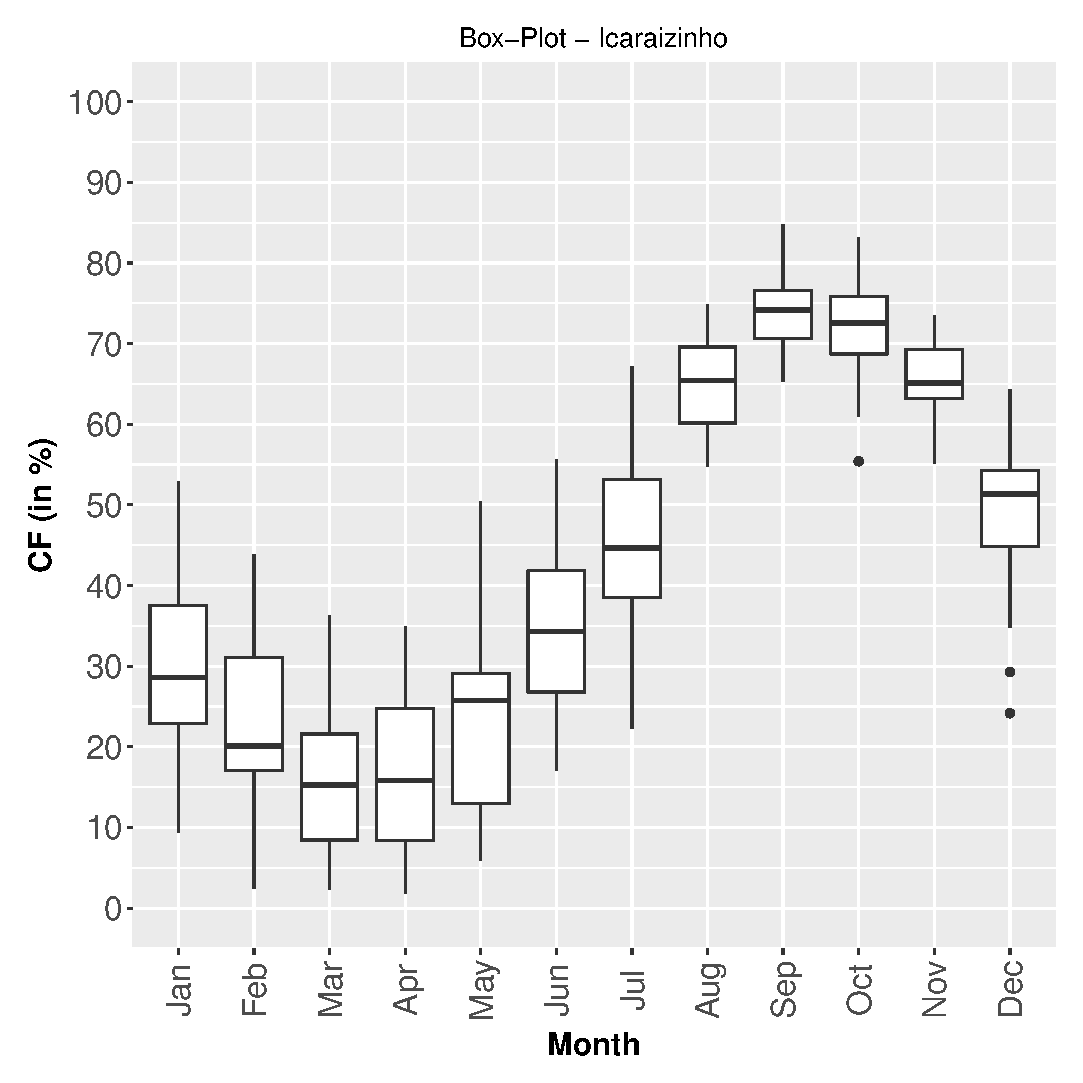
\includegraphics[height=7cm,width=7cm]{figures/BOXPLOT_IC.eps}
%\caption{Monthly capacity factor from a wind plant located at the Northest of Brazil. The time series ranges from January 1981 to December 2011.}
%\label{BoxPlots_IC_mensal}
%\end{figure}

%\begin{figure}[htbp]
%\centering
%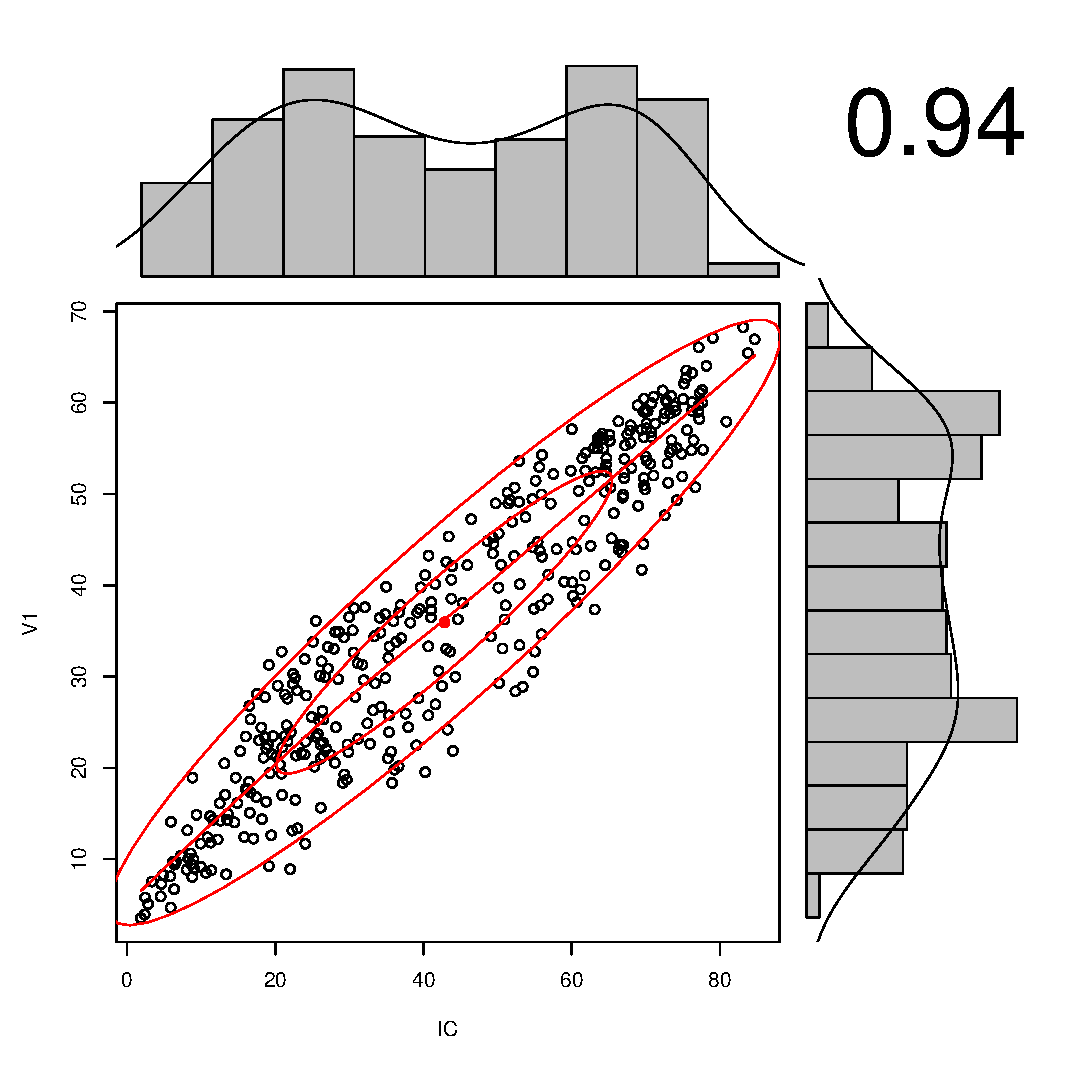
\includegraphics[height=5cm,width=6cm]{figures/HIST_ENxIC.eps}
%\caption{Scatterplot+Histogram ENxIC}
%\label{BoxPlots}
%\end{figure}
%
%\begin{figure}[htbp]
%\centering
%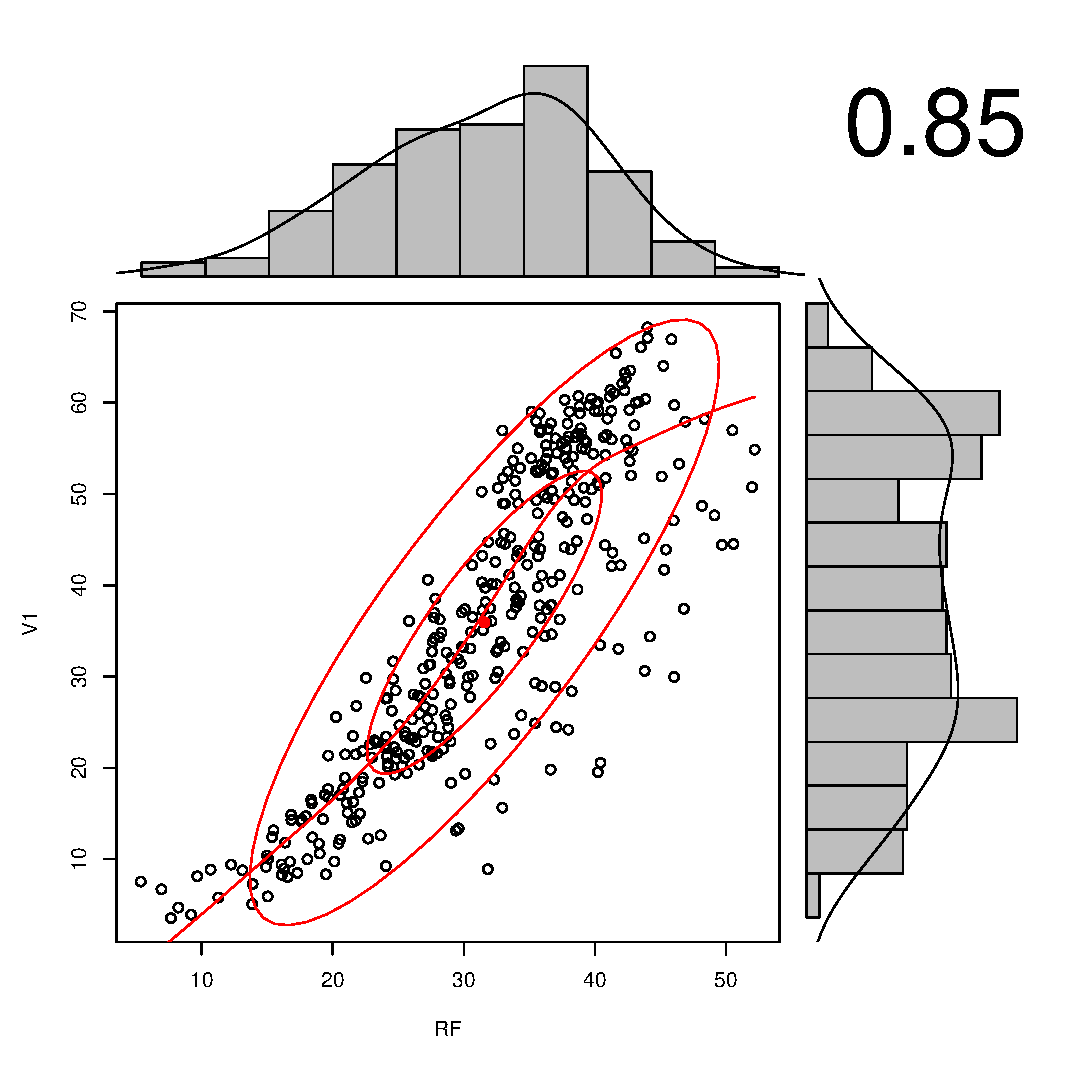
\includegraphics[height=5cm,width=6cm]{figures/HIST_RFxEN.eps}
%\caption{Scatterplot+Histogram RFxEN}
%\label{BoxPlots}
%\end{figure}
%
%\begin{figure}[htbp]
%\centering
%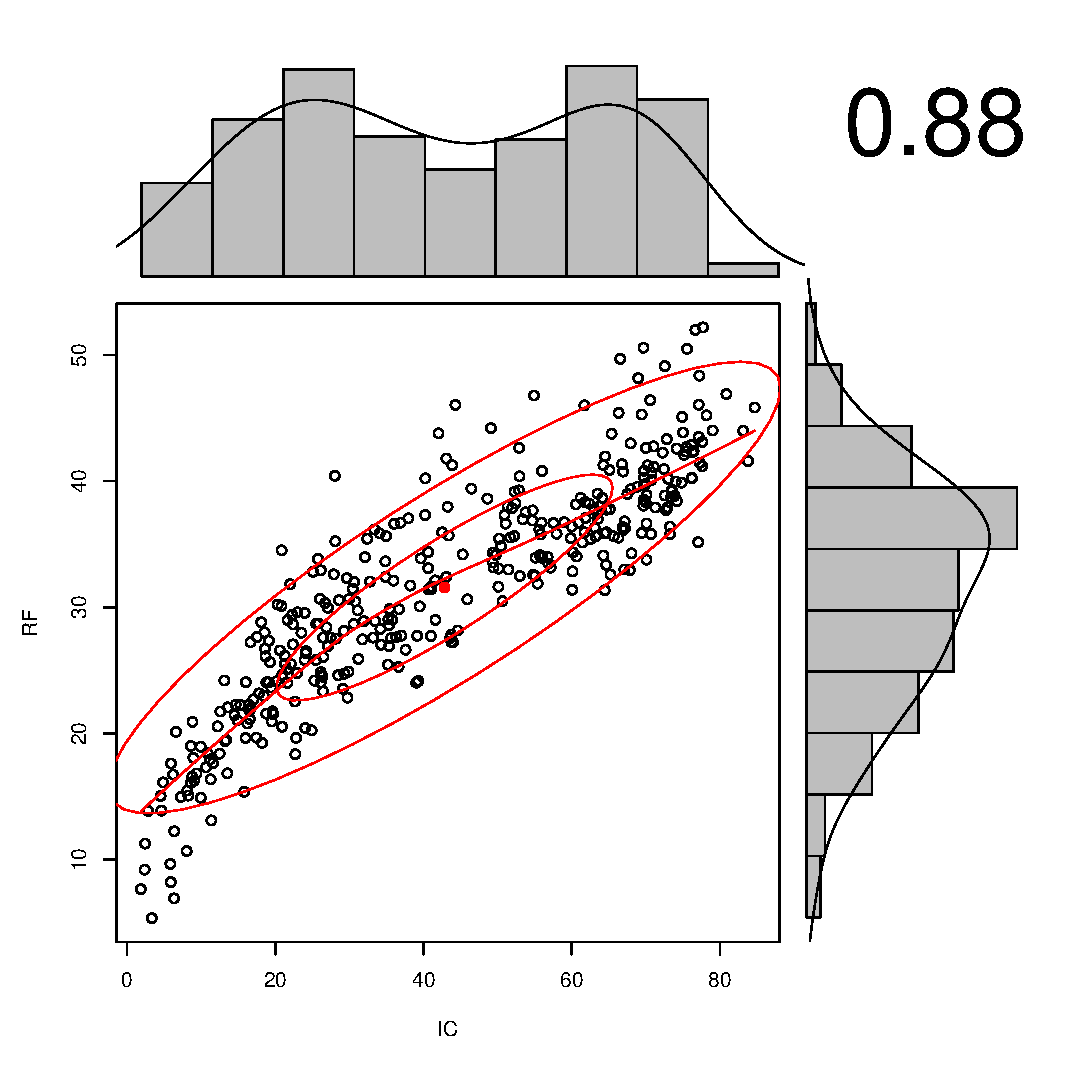
\includegraphics[height=5cm,width=6cm]{figures/HIST_RFxIC.eps}
%\caption{Scatterplot+Histogram RFxIC}
%\label{BoxPlots}
%\end{figure}
%
%
%
%\begin{figure}[htbp]
%\centering
%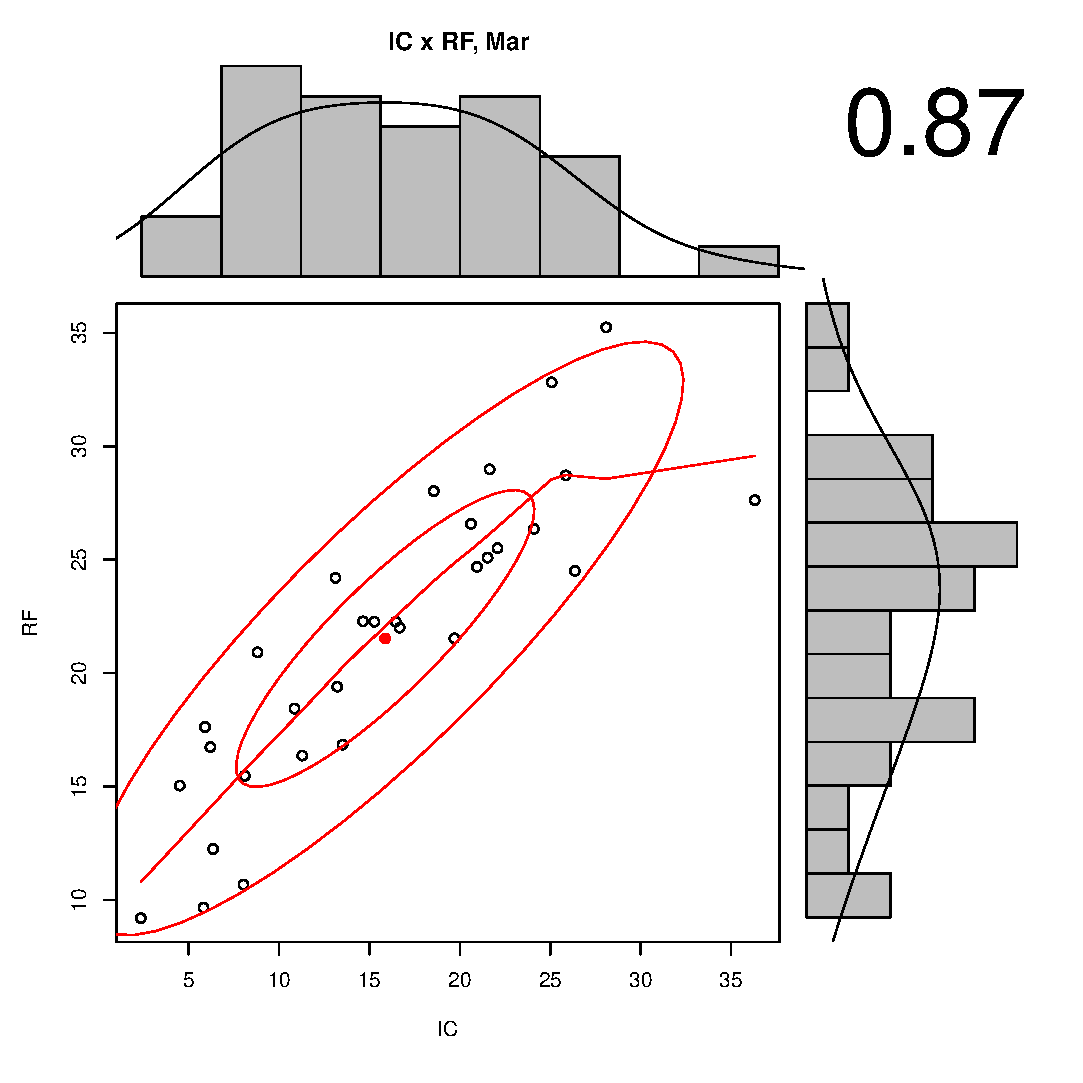
\includegraphics[height=2cm,width=2cm]{figures/HIST_ICxRF_mesMar.eps}
%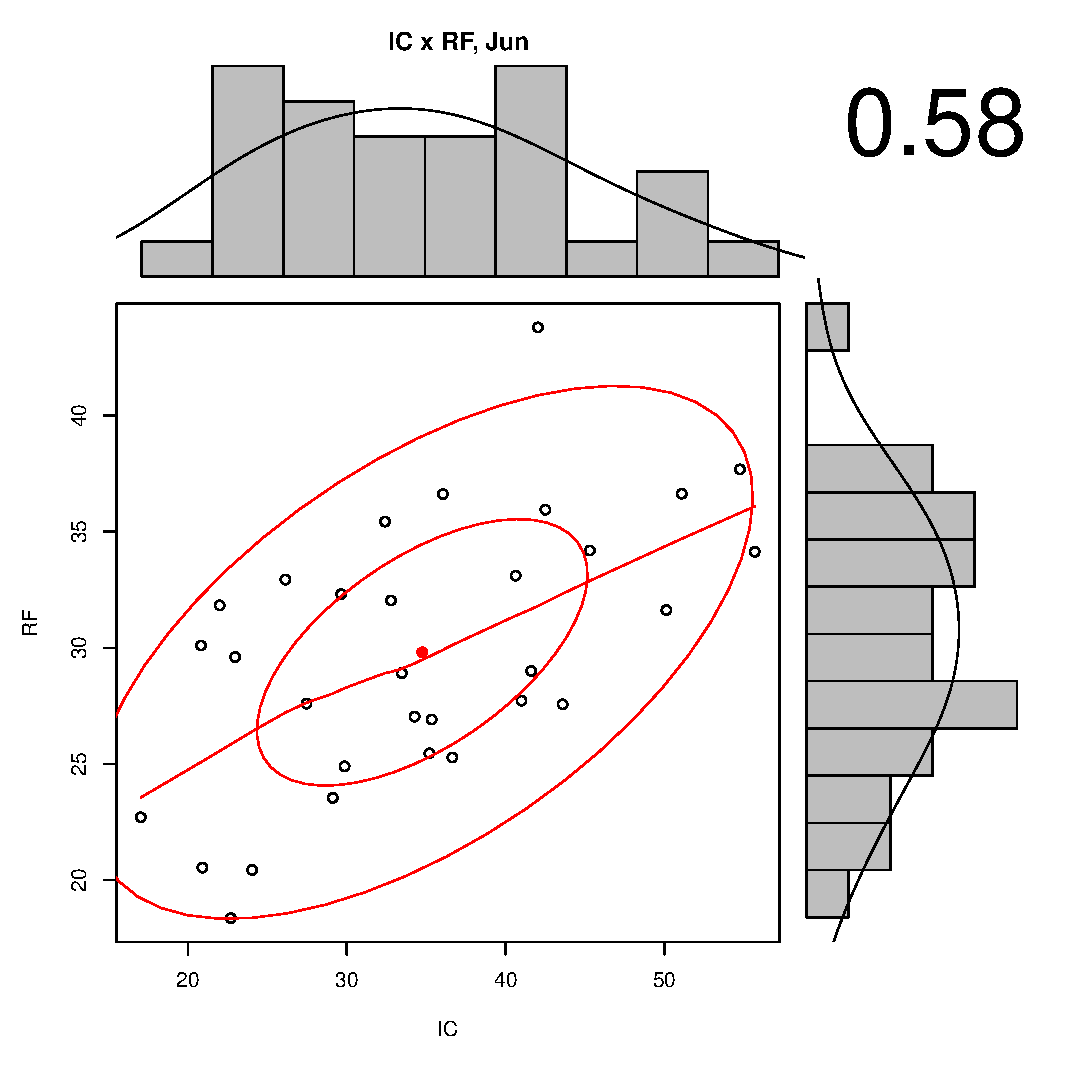
\includegraphics[height=2cm,width=2cm]{figures/HIST_ICxRF_mesJun.eps}
%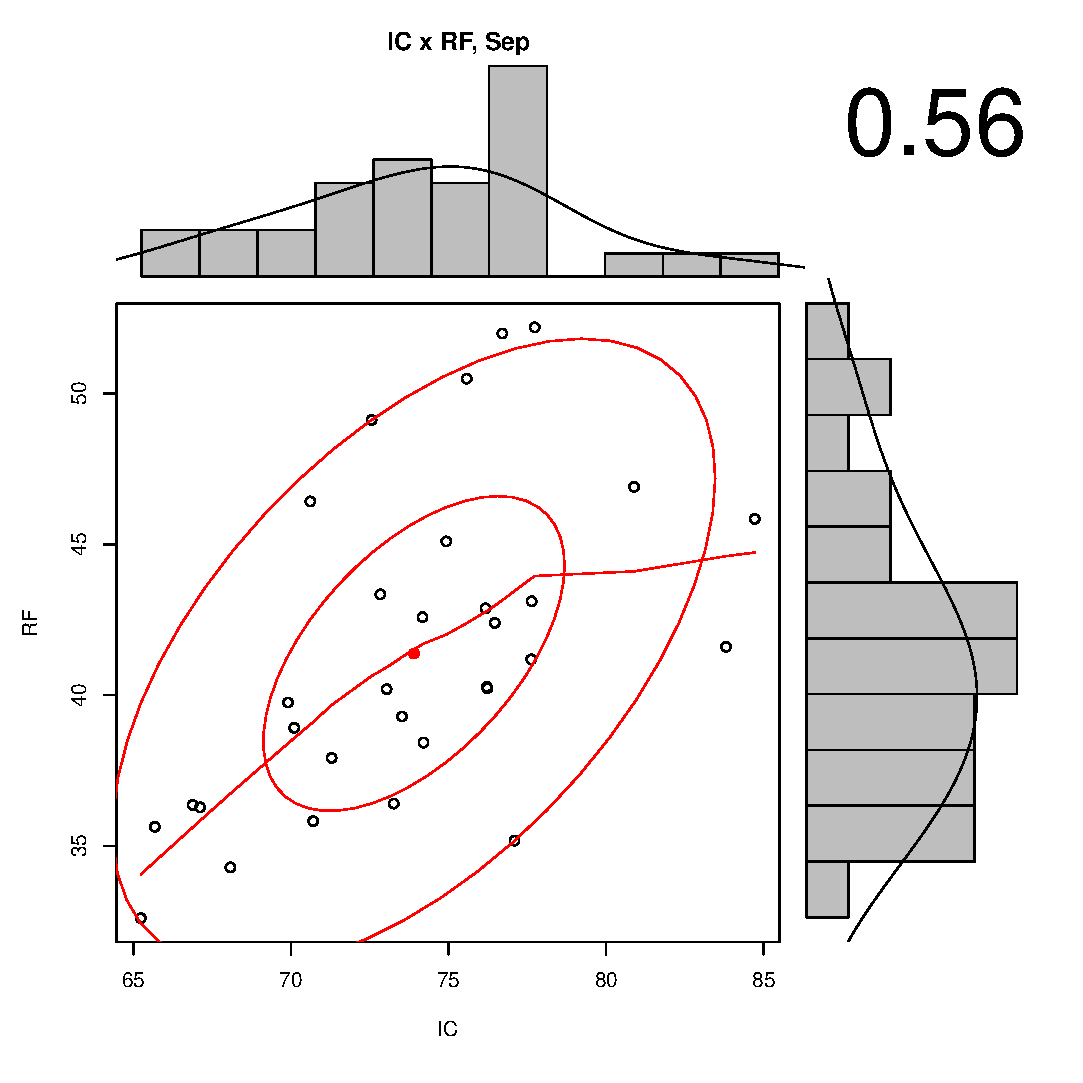
\includegraphics[height=2cm,width=2cm]{figures/HIST_ICxRF_mesSep.eps}
%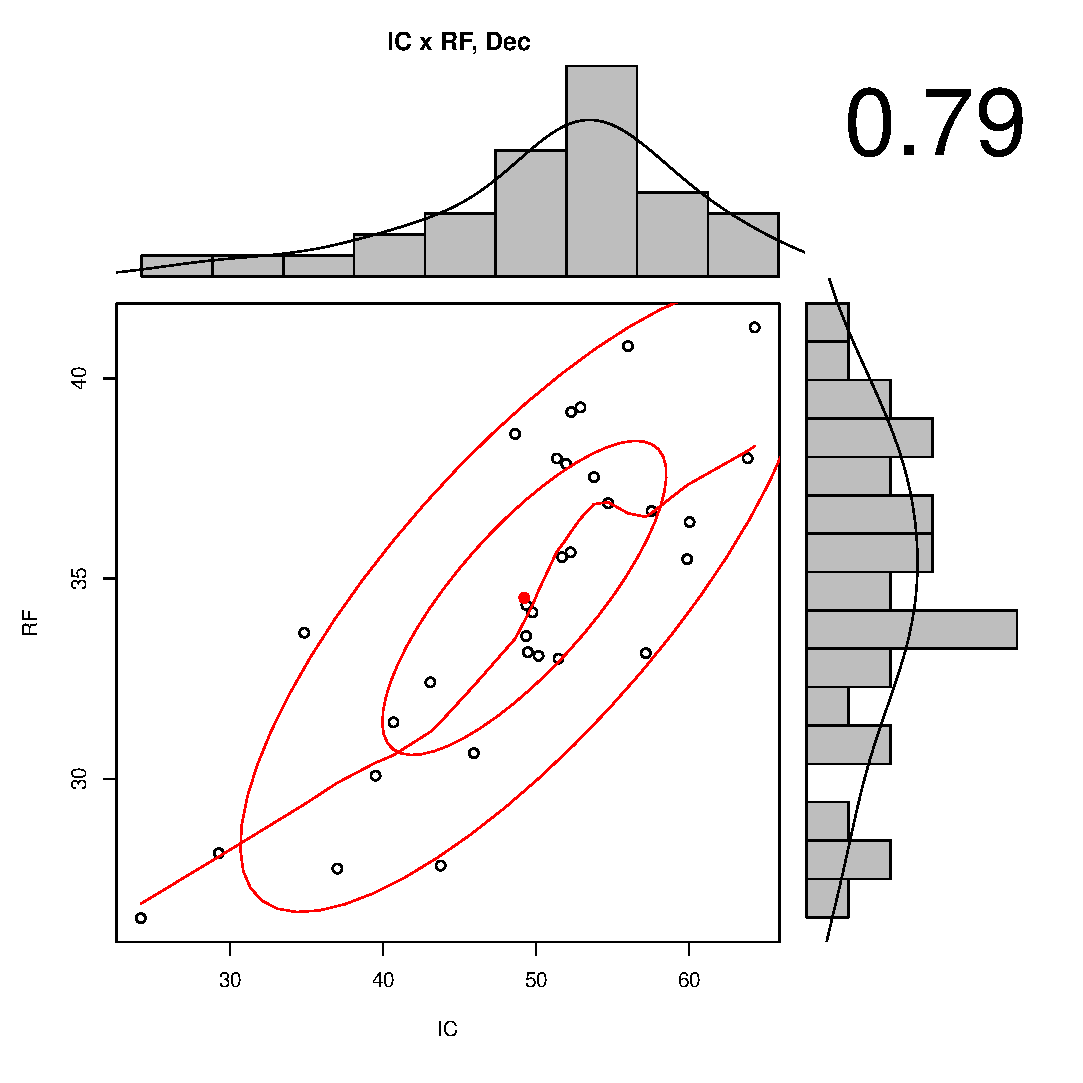
\includegraphics[height=2cm,width=2cm]{figures/HIST_ICxRF_mesDec.eps}
%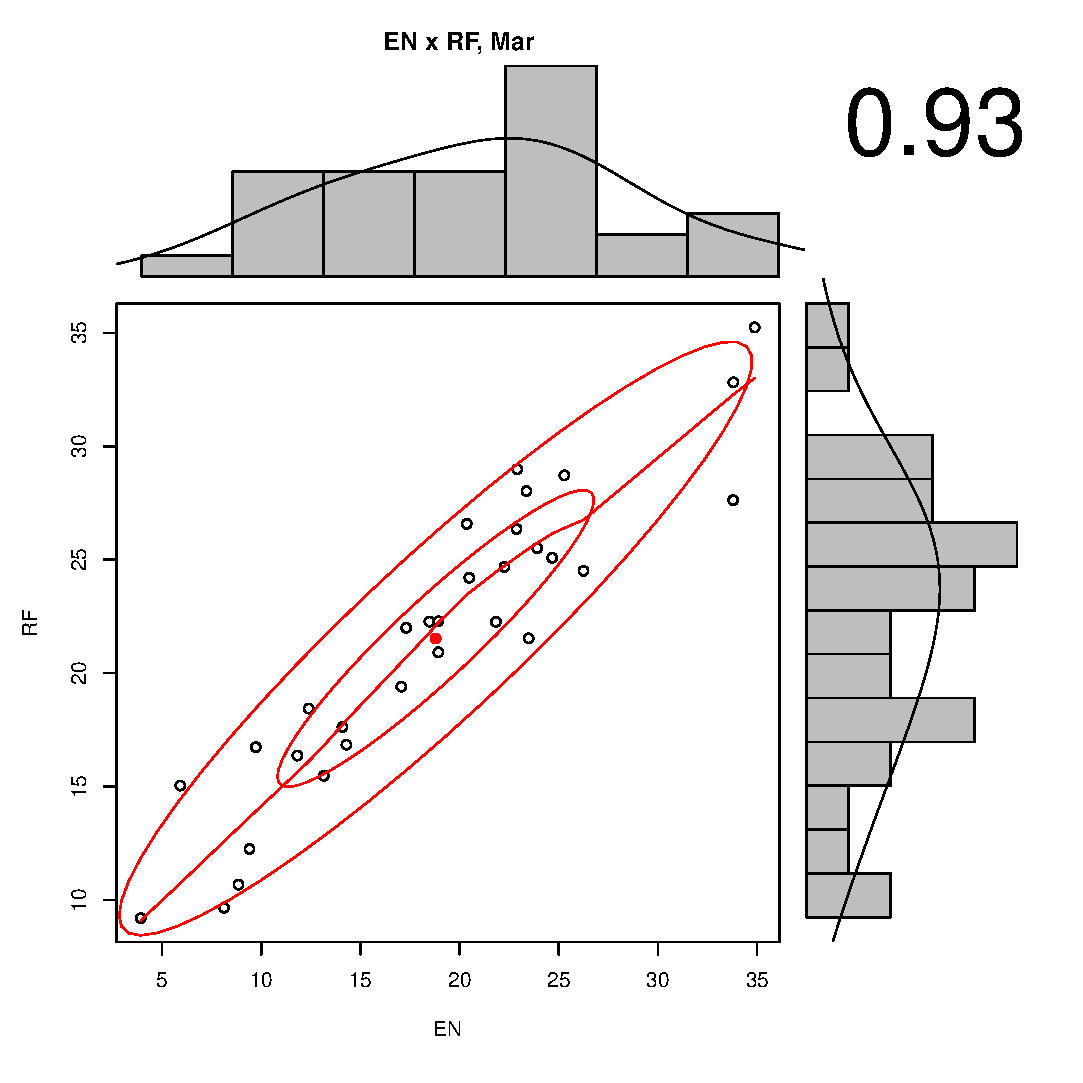
\includegraphics[height=2cm,width=2cm]{figures/HIST_ENxRF_mesMar.eps}
%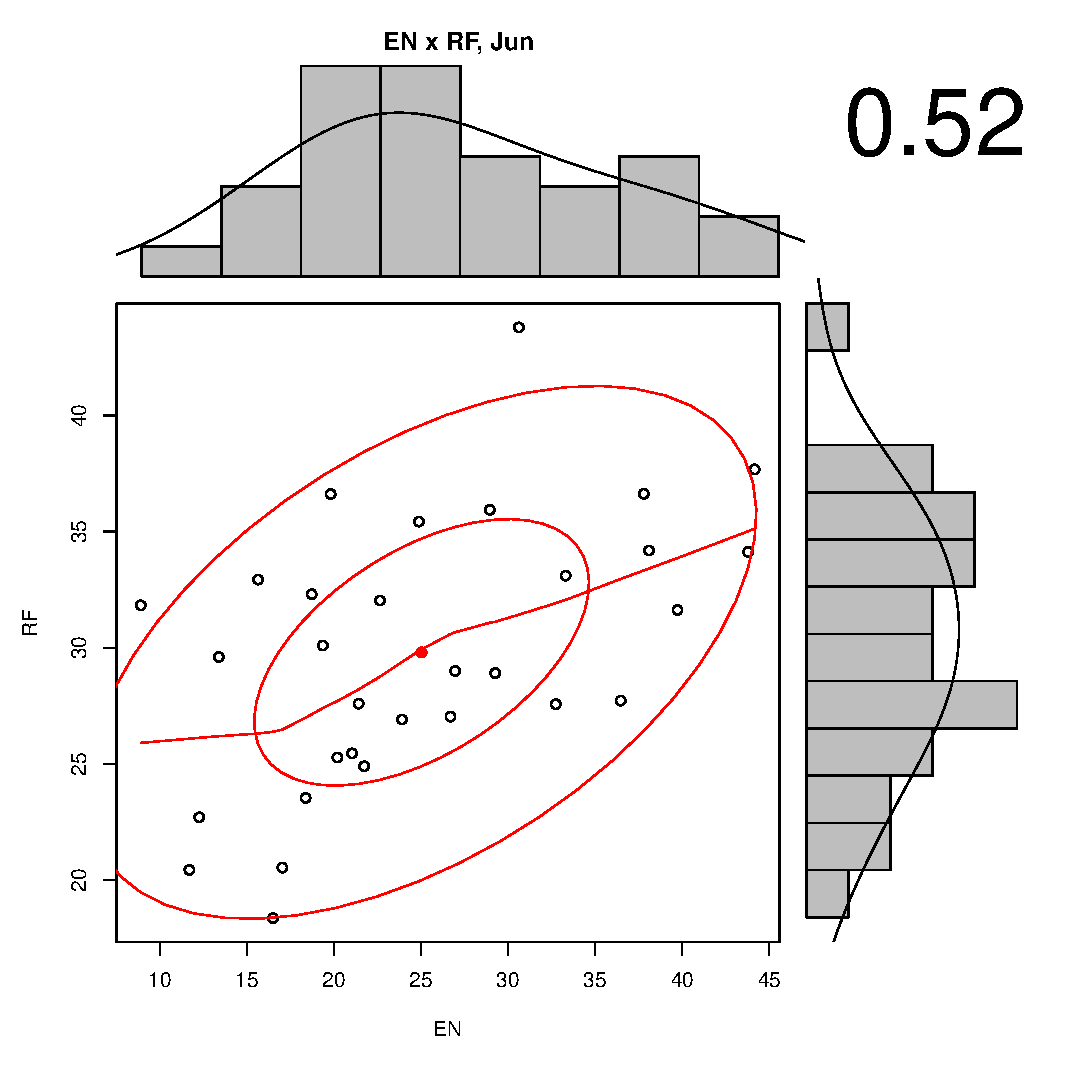
\includegraphics[height=2cm,width=2cm]{figures/HIST_ENxRF_mesJun.eps}
%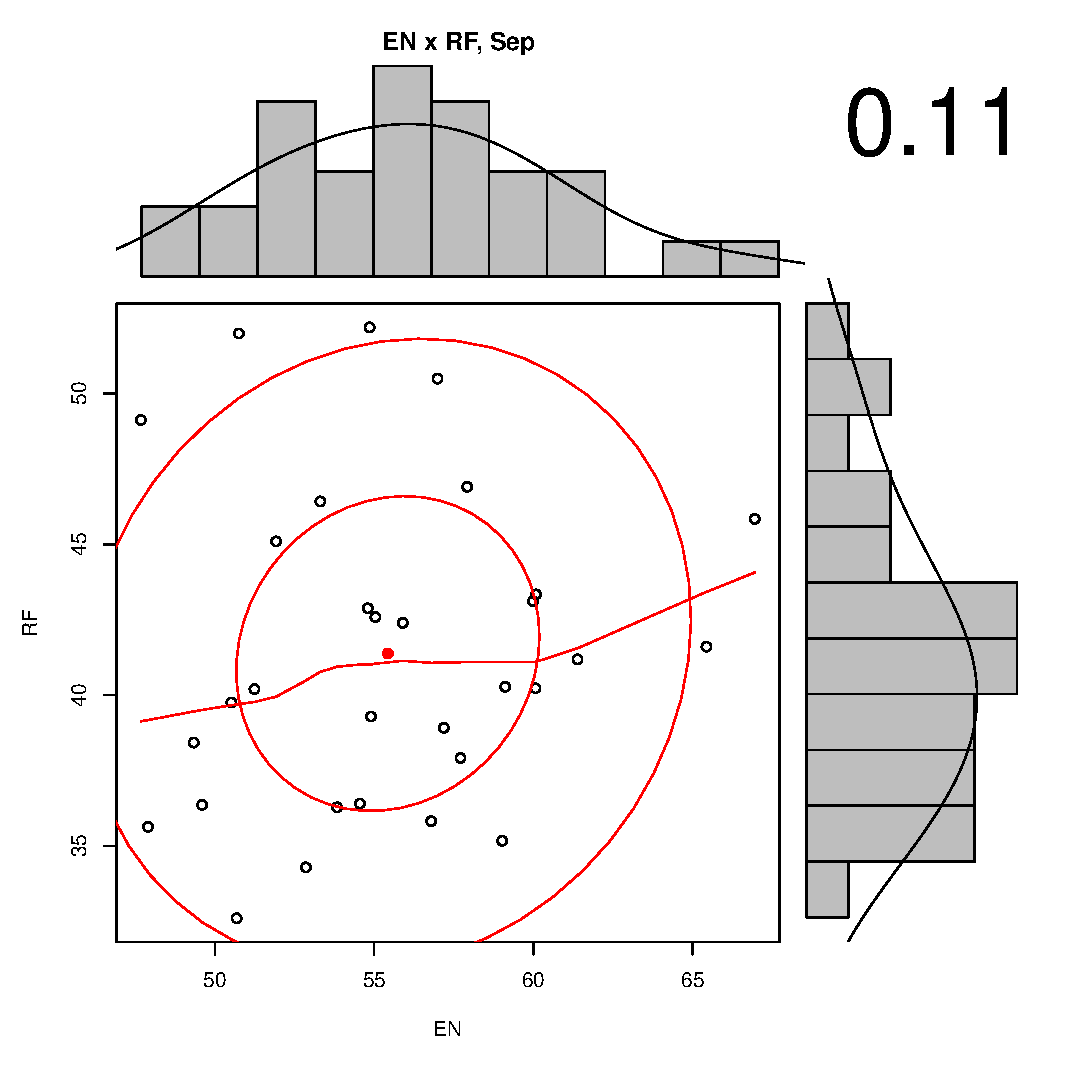
\includegraphics[height=2cm,width=2cm]{figures/HIST_ENxRF_mesSep.eps}
%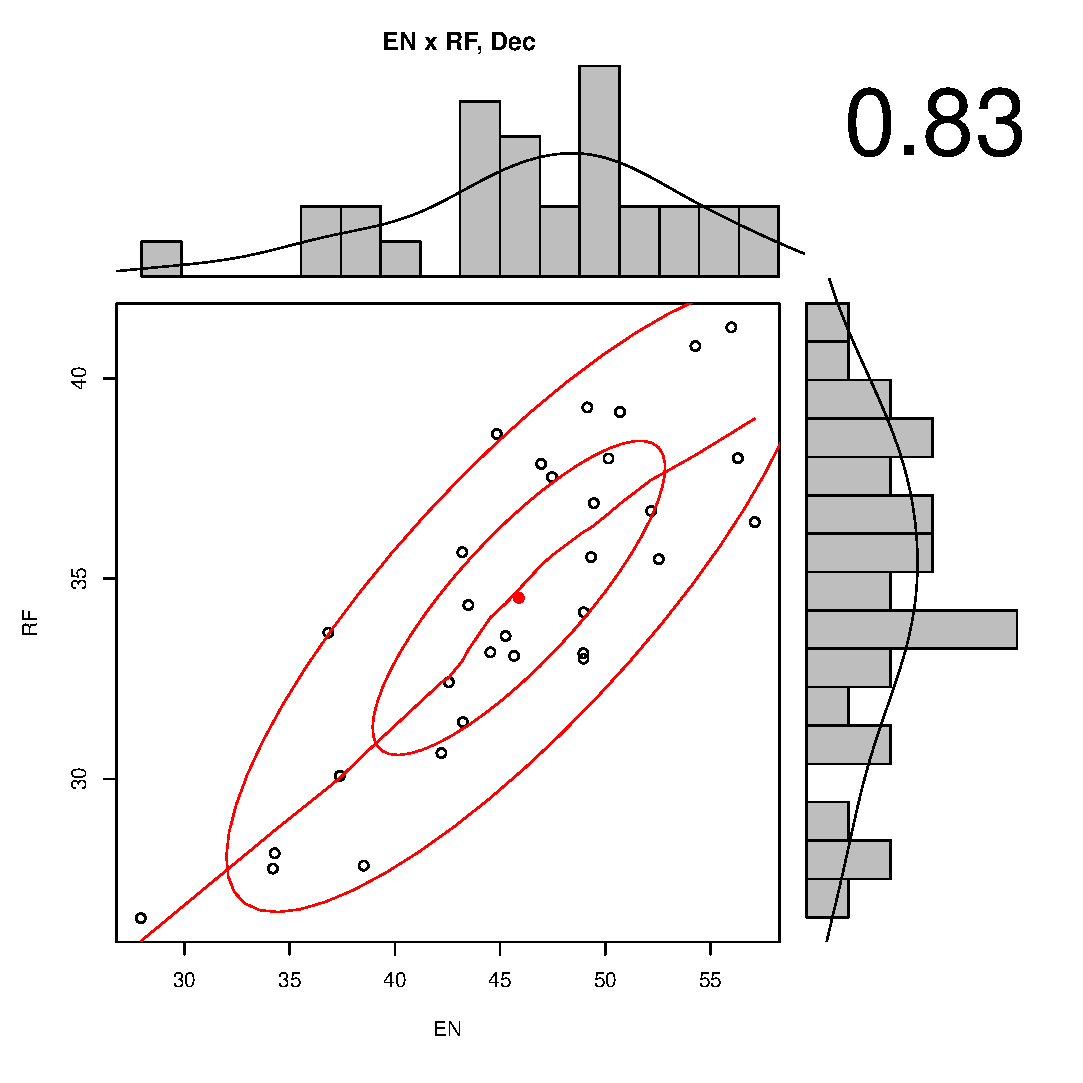
\includegraphics[height=2cm,width=2cm]{figures/HIST_ENxRF_mesDec.eps}
%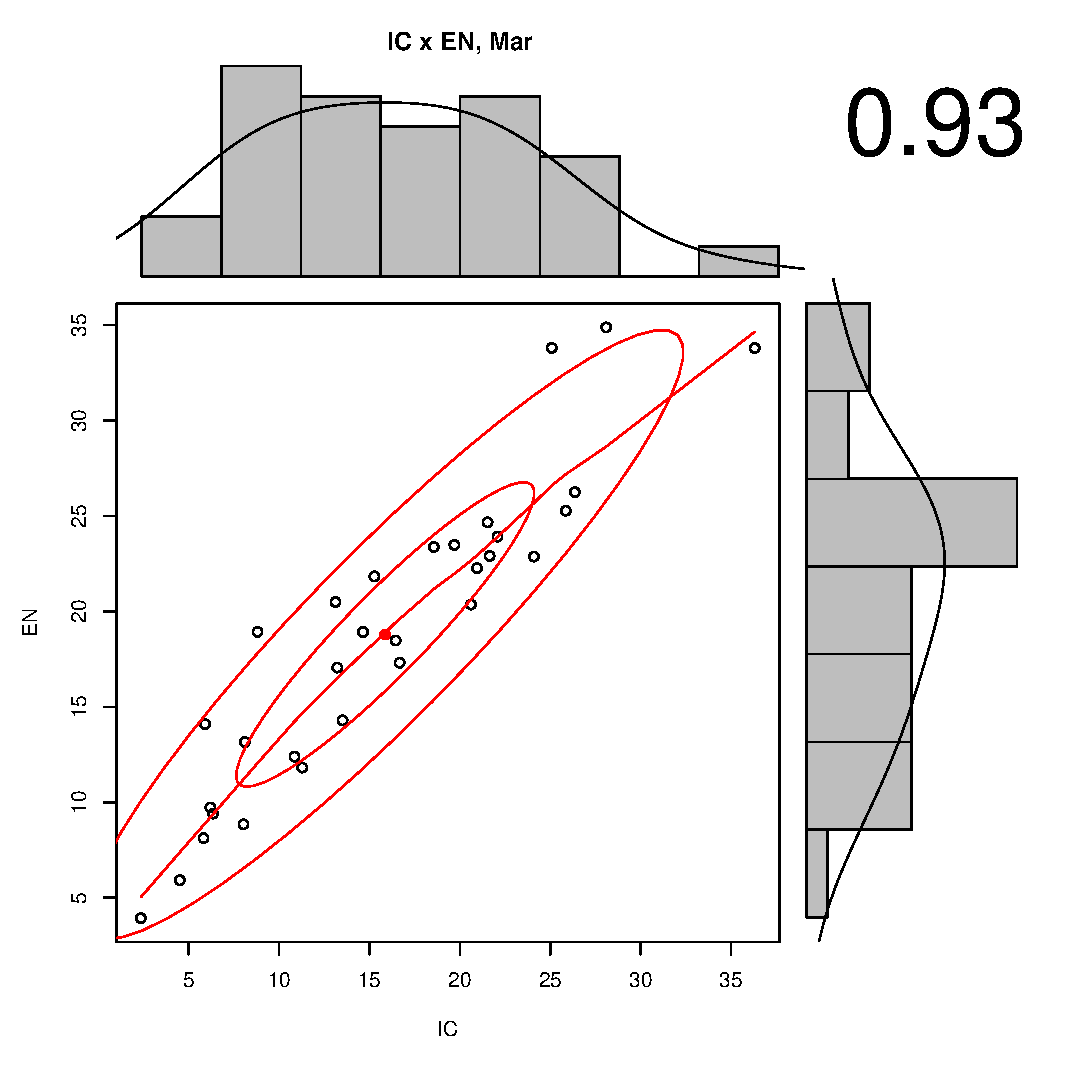
\includegraphics[height=2cm,width=2cm]{figures/HIST_ICxEN_mesMar.eps}
%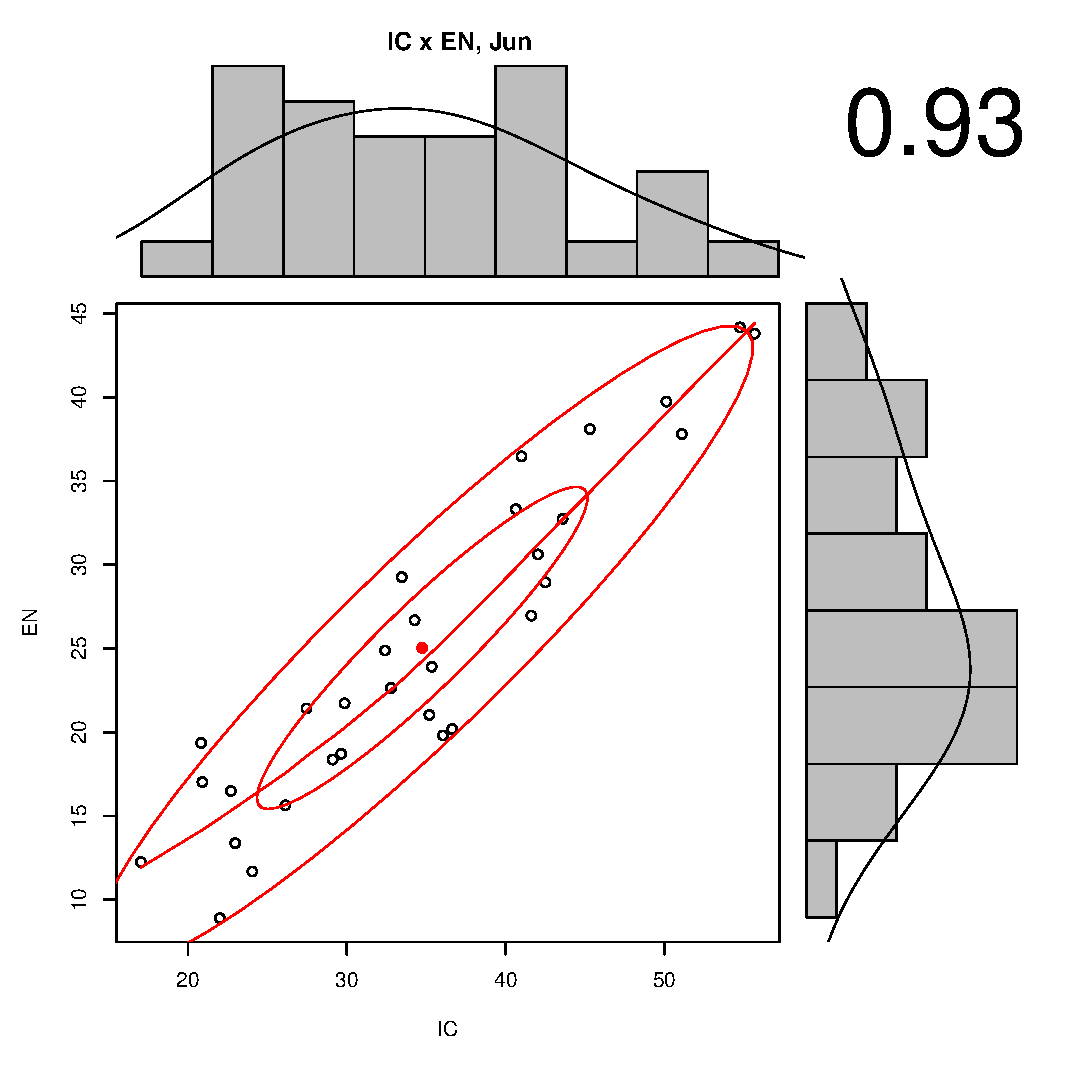
\includegraphics[height=2cm,width=2cm]{figures/HIST_ICxEN_mesJun.eps}
%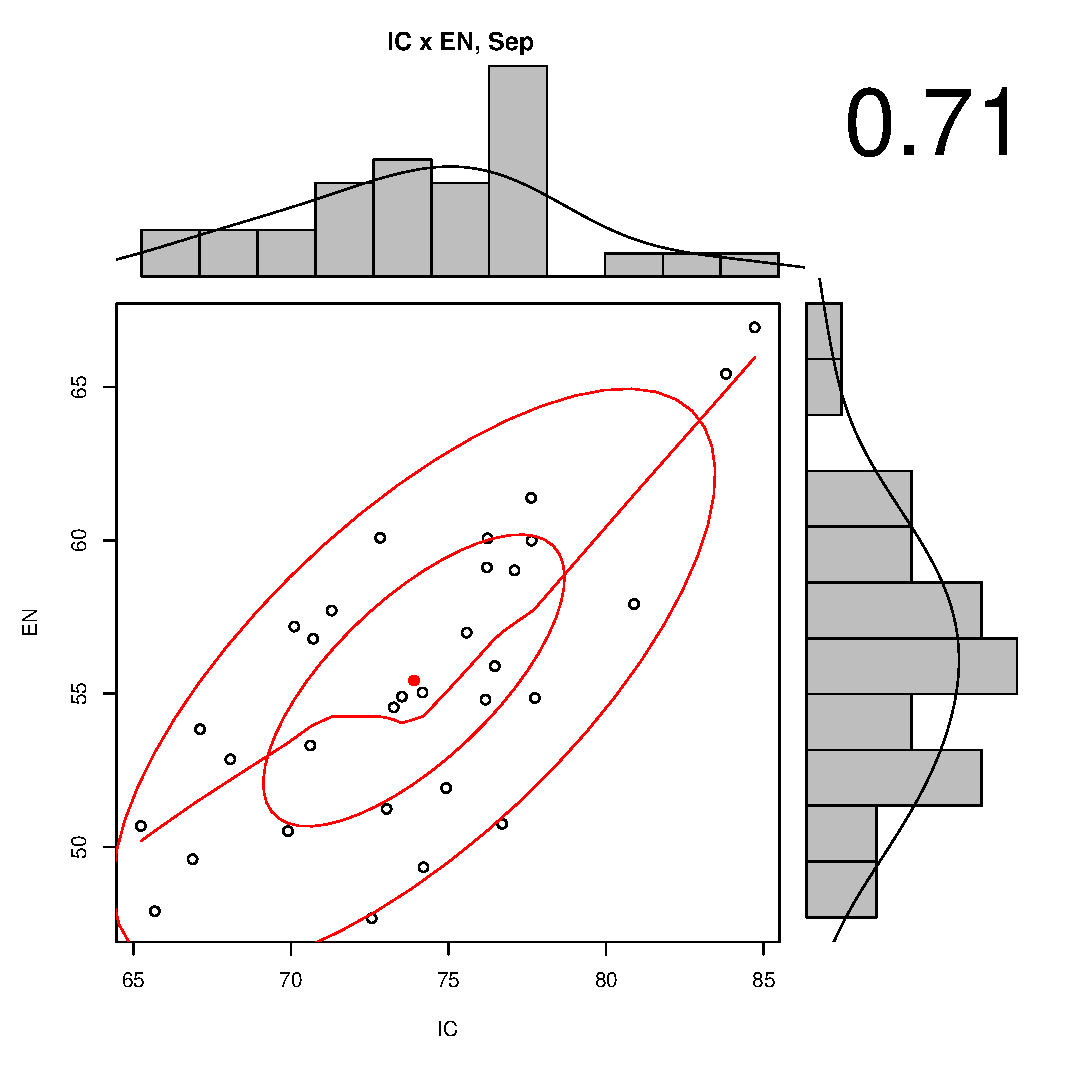
\includegraphics[height=2cm,width=2cm]{figures/HIST_ICxEN_mesSep.eps}
%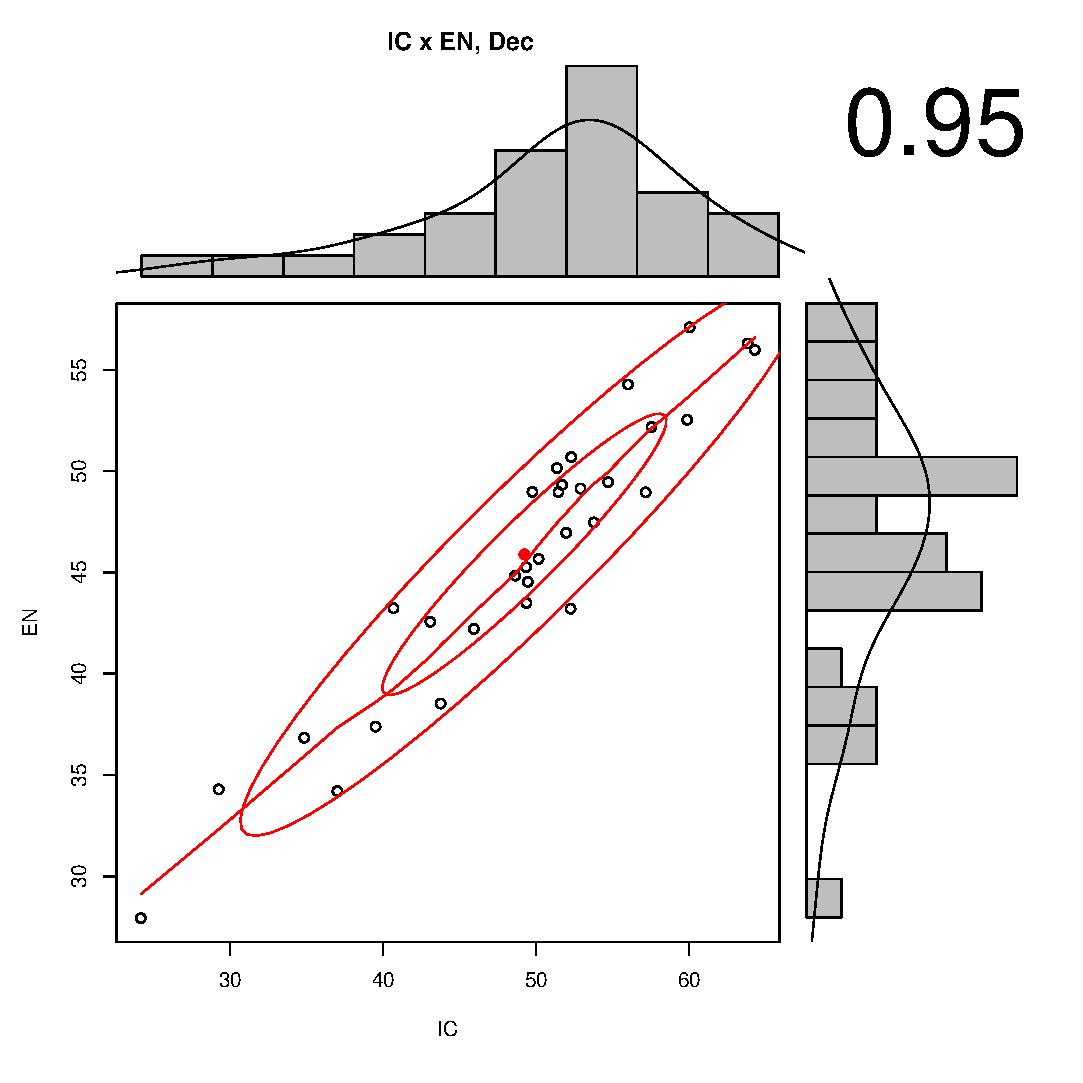
\includegraphics[height=2cm,width=2cm]{figures/HIST_ICxEN_mesDec.eps}
%\caption{Montly Histogram + Scatterplot}
%\label{hist_Scatter}
%\end{figure}




%\begin{figure}[htbp]
%\centering
%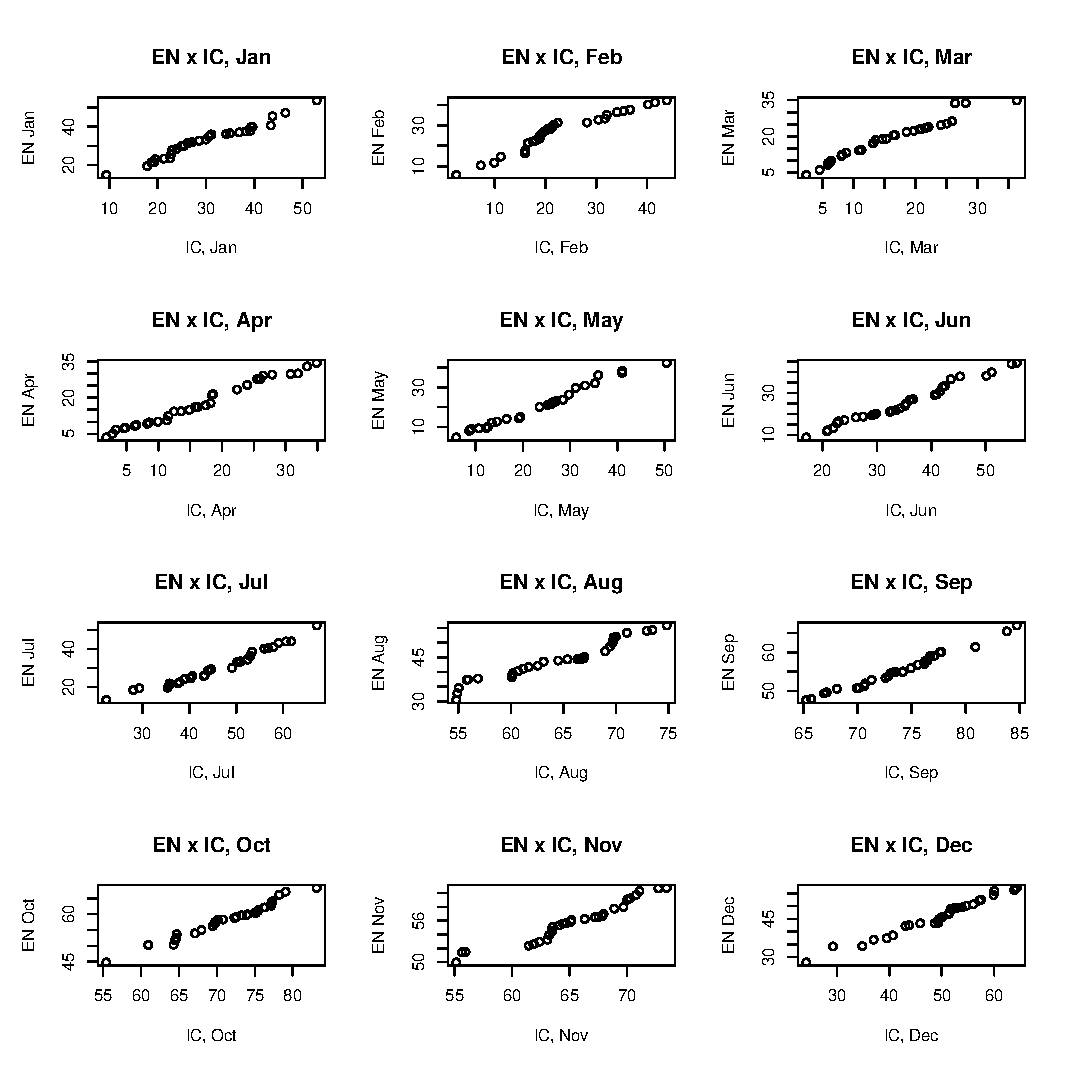
\includegraphics[height=10cm,width=9cm]{figures/ENxIC_MES.eps}
%\caption{Monthly qqplot ENxIC.}
%\label{BoxPlots}
%\end{figure}
%
%\begin{figure}[htbp]
%\centering
%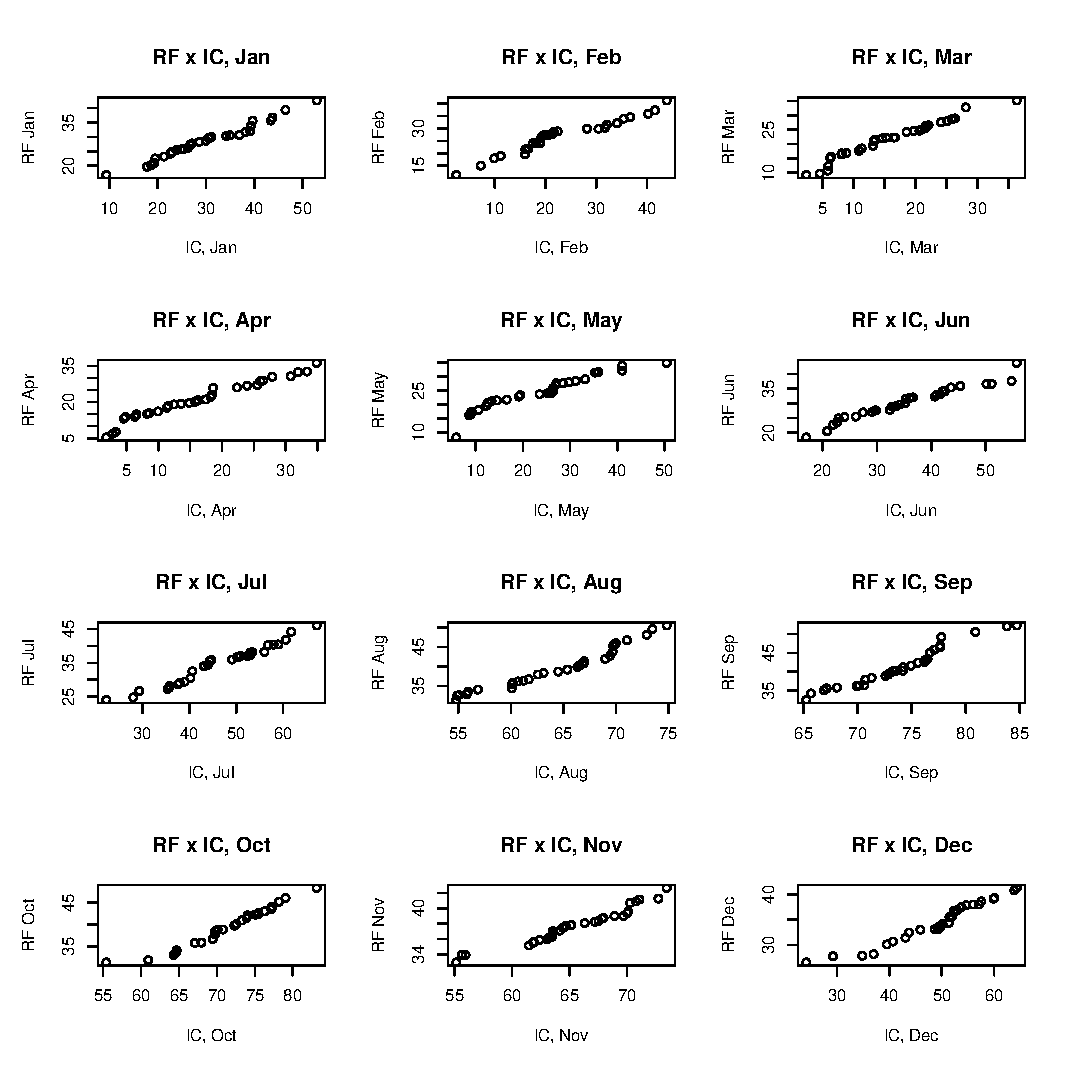
\includegraphics[height=10cm,width=9cm]{figures/RFxIC_MES.eps}
%\caption{Monthly qqplot RFxIC.}
%\label{BoxPlots}
%\end{figure}
%
%\begin{figure}[htbp]
%\centering
%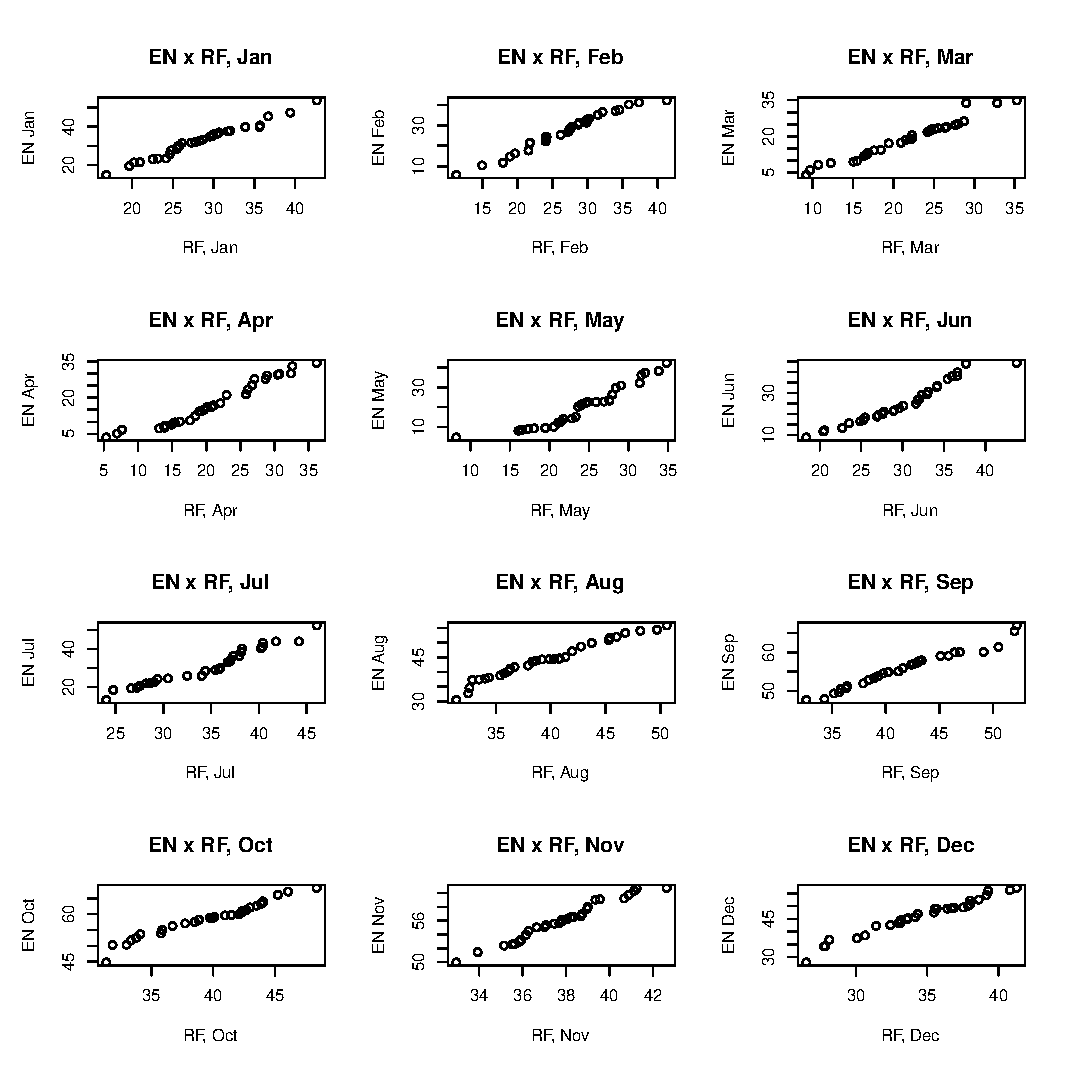
\includegraphics[height=10cm,width=9cm]{figures/RFxEN_MES.eps}
%\caption{Monthly qqplot RFxEN.}
%\label{BoxPlots}
%\end{figure}
%
%\begin{figure}[htbp]
%\centering
%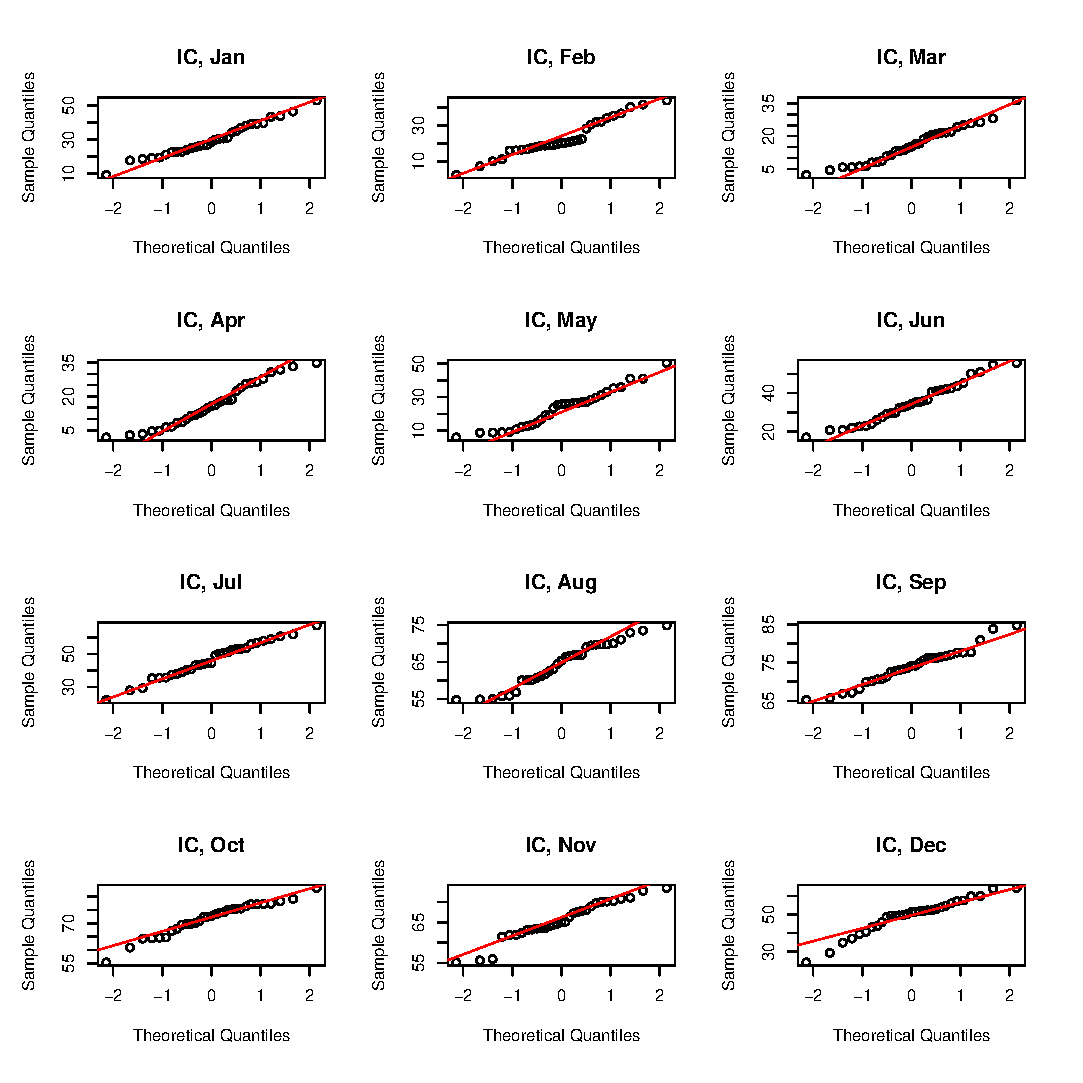
\includegraphics[height=10cm,width=9cm]{figures/IC_QQ_MES.eps}
%\caption{qqplot IC}
%\label{BoxPlots}
%\end{figure}
%
%
%\begin{figure}[htbp]
%\centering
%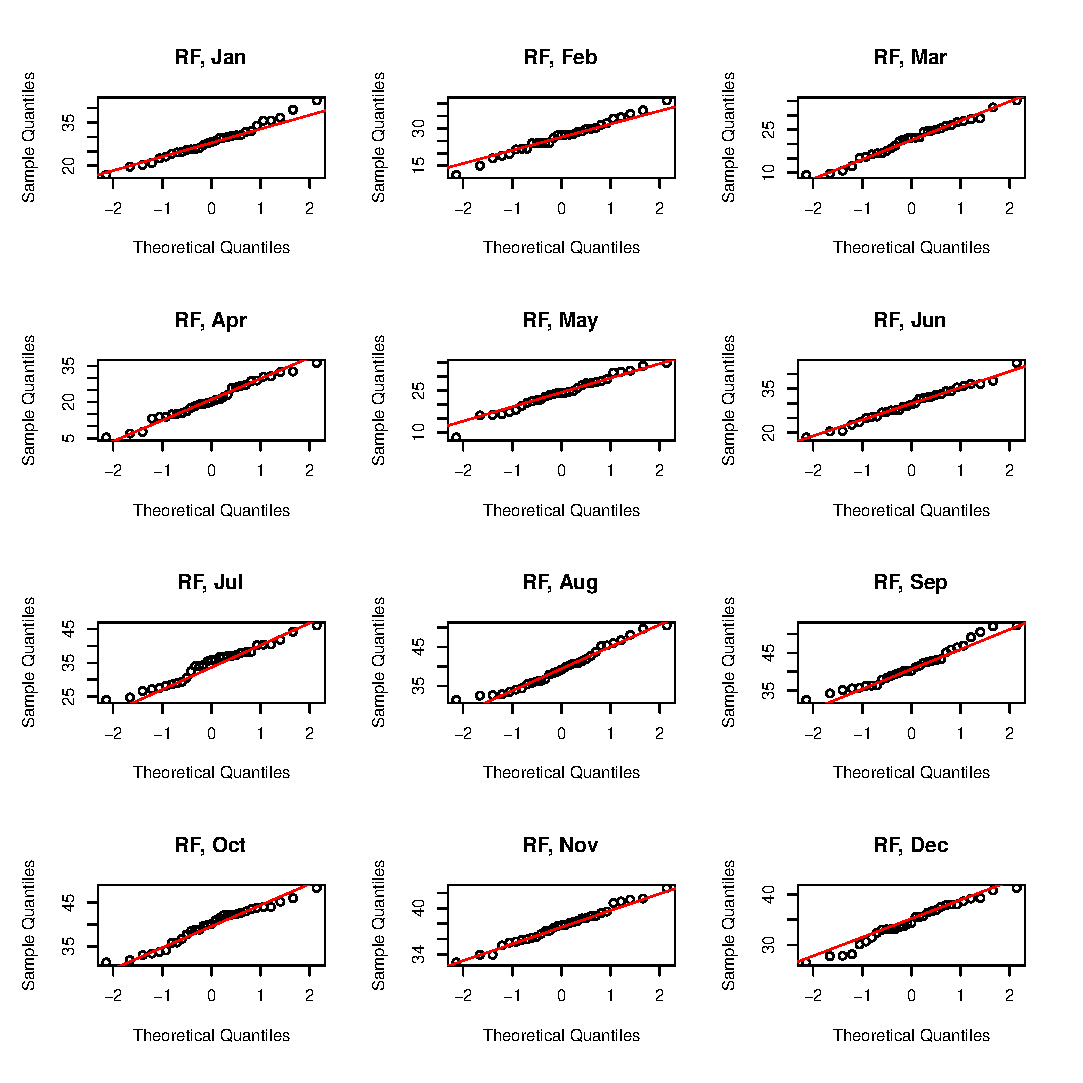
\includegraphics[height=10cm,width=9cm]{figures/RF_QQ_MES.eps}
%\caption{qqplot RF}
%\label{BoxPlots}
%\end{figure}
%
%\begin{figure}[htbp]
%\centering
%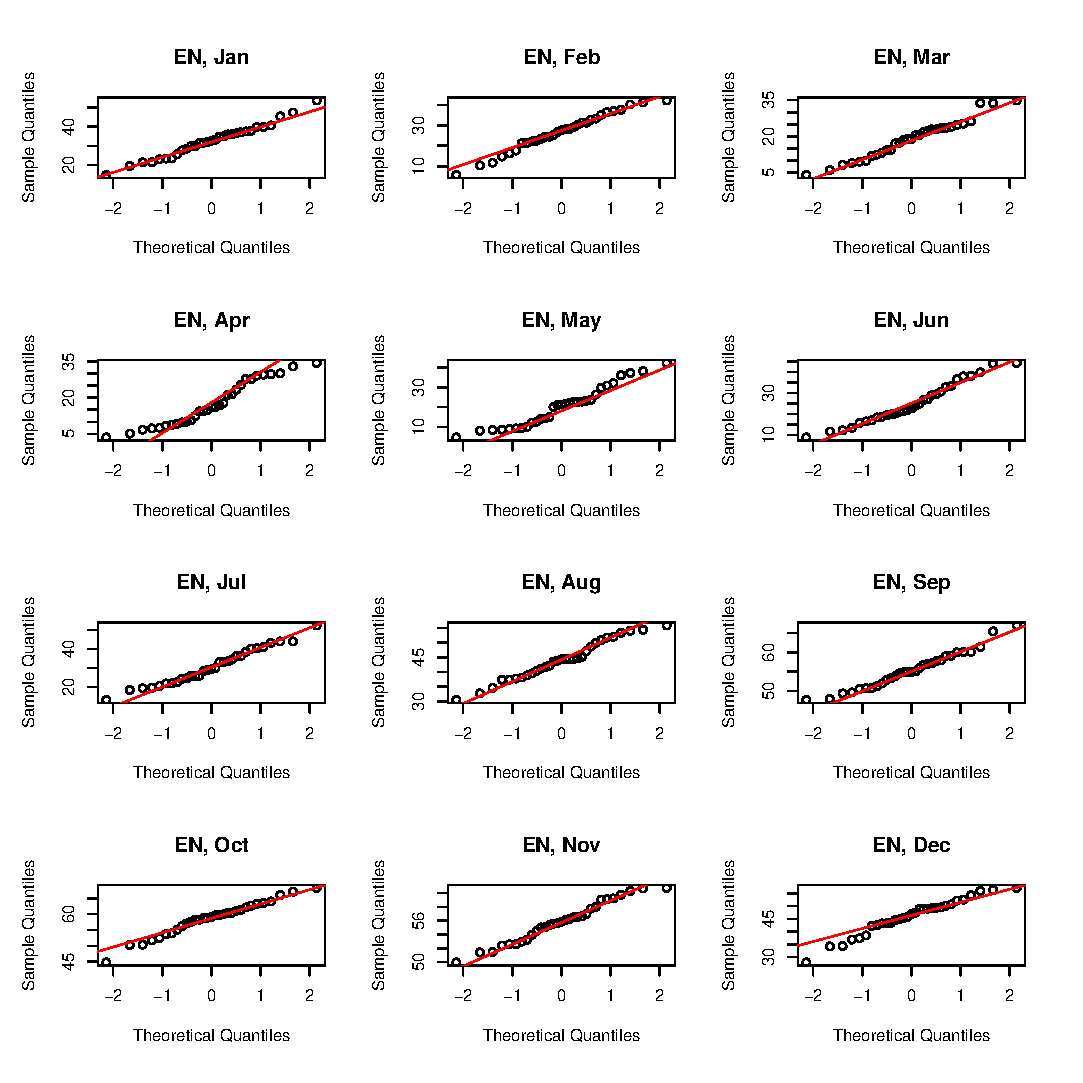
\includegraphics[height=10cm,width=9cm]{figures/EN_QQ_MES.eps}
%\caption{qqplot EN}
%\label{BoxPlots}
%\end{figure}

%\begin{table}[ht]
%\centering
%\caption{P-values of Jarque Bera test of Normality applied to each month time series.}
%\begin{tabular}{rrrrr}
%  \hline
% & Mar & Jun & Sep & Dec \\ 
%  \hline
%  IC & 0.63 & 0.57 & 0.91 & 0.13 \\ 
%  RF & 0.82 & 0.96 & 0.46 & 0.58 \\ 
%  EN & 0.82 & 0.45 & 0.60 & 0.42 \\ 
%   \hline
%\end{tabular}
%\end{table}

%In addition to the strong seasonal pattern presented by Figure \ref{BoxPlots_IC_mensal}, another important stylized fact of CF time series is provided, season effects. During the first half of the year, wind speed tends to decrease and also its frequency. As an outcome, the CF of these months will naturally drop. On the other hand, during the second semester, the opposite happens.




%and the non Gaussian pattern of such variable, which is statistically confirmed by the
%Another evidence, which corroborates with our Moreover, checking each month empirical density, it is possible to conclude that they are asymmetric, and when calculating theirs values, August`s skewness is the closest to zero, in modulus, with a value of 0.1306.

%DIF < Tradicionalmente, tem-se utilizado modelos ARMA e seus derivados, os quais pressupoe a hipotese de normalidade da serioe, o que contraria os fatos estilizados ja elucidados. Mesmo trabalhando com o log da serie, problemas persistem, pois como o objetvio é a simulacao na escala original da série, observa-se que ao se aplicar a exponenciacao, as simulacoes da serie obtida pelo modelo arma gaussiano, a magnitude dos valres simulados muitas vezes sao superiores aos valores historicamente observados
%DIF > Tradicionalmente, tem-se utilizado modelos ARMA e seus derivados, os quais pressupoe a hipotese de normalidade da serioe, o que contraria os fatos estilizados ja elucidados. Mesmo trabalhando com o log da serie, problemas persistem, pois como o objetvio é a simulacao na escala original da série, observa-se que ao se aplicar a exponenciacao, as simulacoes da serie obtida pelo modelo arma gaussiano, a magnitude dos valres simulados muitas vezes sao superiores aos valores historicamente observados

%The non Gaussian nature of CF time series, in most applications in the energy literature, is not directly dealt with, either because of non availability of proper software or by the computational burden in implementing existing non Gaussian models. For example, if one decides to fit a non-Gaussian state space model using unobserved components, such as trend, seasonals and cycle, it would be necessary extensive Monte Carlo simulation for both state and fixed parameter estimation. See, for example, Durbin and Koopman (2012, pp 209-324). In practice a great deal of applied work involving scenario generation for wind speed or CF time series make use of ARMA models and its extensions, \cite{box1976time}, mostly under normality assumption. At best such models are fitted to the log of the variable of interest, and by taking the anti log, predictions and simulations on the original scale of the variable are obtained. Unfortunately such a strategy can result in unrealistic sampling paths for the original variable.

%Hence, the need to apply the $log$ transformation and then fit the data properly. Yet, it is also a non conventional form, as it is known, to come back to the original scale, it is necessary the exponentiation of simulated Gaussian values that can result in unrealistic sampling paths as can be seen in Figure \ref{SARIMA_COM_TRANS} where we simulate 2000 scenarios 12 steps ahead.




%, and by propagation, this can badly affect the risk measures obtained from the simulated distribution of the cash flows associated with a particular portfolio of wind plants. %our approach can generate scenarios in just one step, avoiding the need of transforming back the outcome variables to its original scale, as it is the case under a Gaussian assumption for the marginal models. As it is known, exponentiation of simulated Gaussian values can result in unrealistic sampling paths for the wind capacity factor. 

%Isso cria uma motivacao para o estabelecimento de modelos que sejam capazes de modelar series nao gaussianas e que contemplem a questao de nao linearidade

%Such features motivates the insertion of a recently proposed time series framework which gracefully handles with the two aforementioned challenges. In this paper we applied to monthly  wind capacity factor (CF) time series a newly proposed class of observation-driven time series models, the so called GAS models \cite{creal2013generalized} or Dynamic Conditional Score (DCS), following \cite{harvey2013dynamic}. Our approach fits in the classification proposed by \cite{zhang2014review} as a long-term parametric probabilistic. More specifically one can pick any desirable predictive distribution judged appropriate for the response variable being modelled and, trough the dynamic equations proposed in the GAS frameworks, make its parameters time varying. We advocate that wind probabilistic forecasting should be preferred in practice since from it, apart from conditional measures of location, like mean or median, one can obtain many different measures of interest, like conditional quantiles, enabling improved decision making to power systems operators and investors.

%However, for several applications, such as unit commitment, regulation and commercialization, these variables are plugged into the power curve to transform wind speed/wind power into a CF time series. The models here proposed are directly fitted to the CF time series which are directly available, and as consequence  no such transformations will be needed. \cite{zhang2014review} presents a detailed review of state-of-the-art methods and new developments in wind power uncertainty forecasting. 
%As \cite{mur2010variability} conclude, wind power generation is a non-linear and non-stationary process, which are also features of wind speed time series. Therefore common choices of models that could reproduce its pattern use time series models (e.g. \cite{brown1984time}) or Artificial Intelligence \cite{sideratos2012probabilistic}. 

\DIFdelbegin \DIFdel{Much }\DIFdelend \DIFaddbegin \DIFadd{In contrast to the main objective of WPG simulation methods, which aim to produce scenarios that characterize all the conditional density and its fit to the observed quantile data, much }\DIFaddend research has been devoted to devise short-term forecast methods for wind speed and WPG time series (for instance, see \DIFdelbegin \DIFdel{\mbox{%DIFAUXCMD
\cite{conradsen1984review, brown1984time, conejo2005forecasting,nielsen2006,pinson2007,taylor2009wind,wang2011review,bessa2012time,sideratos2012probabilistic,wan2016,gallego2016line,Xydas2017,cavalcante2017lasso,wang2017deep}
}%DIFAUXCMD
%DIF < \cite{conradsen1984review, brown1984time, conejo2005forecasting,nielsen2006,pinson2007,taylor2009wind,wang2011review,bessa2012time,sideratos2012probabilistic,wan2016,Xydas2017,cavalcante2017lasso,wang2017deep}
and \mbox{%DIFAUXCMD
\cite{zhang2014review}
}%DIFAUXCMD
for a survey on probabilistic forecasting of wind power generation}\DIFdelend \DIFaddbegin \DIFadd{\mbox{%DIFAUXCMD
\cite{zhang2014review}
}%DIFAUXCMD
}\DIFaddend ). In \DIFdelbegin \DIFdel{many applications , the modeling of these time series }\DIFdelend \DIFaddbegin \DIFadd{some applications on medium and long-term forecast, the time series model }\DIFaddend is conducted using conventional ARMA models with seasonal lags, or SARIMA models, under a Gaussian distribution (\DIFdelbegin \DIFdel{\mbox{%DIFAUXCMD
\cite{FosteringWPP,souto2014high}
}%DIFAUXCMD
}\DIFdelend \DIFaddbegin \DIFadd{see \mbox{%DIFAUXCMD
\cite{souto2014high}
}%DIFAUXCMD
for a high-dimension estimation process based on LASSO}\DIFaddend ). In its original formulation, SARIMA models present a fixed \DIFdelbegin \DIFdel{scale parameter}\DIFdelend \DIFaddbegin \DIFadd{conditional variance}\DIFaddend . To add extra flexibility to these models \cite{lau2010approaches} proposes an ARIMA model with GARCH effect, allowing the conditional variance of \DIFdelbegin \DIFdel{wind power }\DIFdelend \DIFaddbegin \DIFadd{the WPG }\DIFaddend distribution to vary over time. Also, to provide a description of the spatial correlation of wind-speed time series, \cite{taylor2009wind} proposed an Autoregressive Fractionally Integrated-GARCH model (ARFIMA-GARCH). In these and other models, conditional on the past, the distribution of the response variable is assumed Gaussian.

The non-Gaussian nature of WPG time series is well reported in the literature (see \cite{bessa2012time,jeon2012using,taylor2015forecasting,Wan2017} \DIFdelbegin \DIFdel{, }\DIFdelend and references therein). \DIFdelbegin \DIFdel{Notwithstanding}\DIFdelend \DIFaddbegin \DIFadd{However}\DIFaddend , only very limited classes of non-Gaussian time-series models \DIFdelbegin \DIFdel{were available for forecasting }\DIFdelend \DIFaddbegin \DIFadd{are available for modeling }\DIFaddend WPG. The state of the art literature on short-term probabilistic \DIFdelbegin \DIFdel{forecast of WPG }\DIFdelend \DIFaddbegin \DIFadd{modeling of WPG time series }\DIFaddend mainly rely on \DIFdelbegin \DIFdel{nonparametric }\DIFdelend \DIFaddbegin \DIFadd{non-parametric }\DIFaddend models. For instance, in \cite{bessa2012time} and \cite{Wan2017}, \DIFdelbegin \DIFdel{nonparametric }\DIFdelend \DIFaddbegin \DIFadd{non-parametric }\DIFaddend approaches were devised to forecast conditional distributions. While in \cite{bessa2012time} kernel density estimators \DIFdelbegin \DIFdel{was }\DIFdelend \DIFaddbegin \DIFadd{were }\DIFaddend employed to build a \DIFdelbegin \DIFdel{density forecast}\DIFdelend \DIFaddbegin \DIFadd{predictive conditional density function}\DIFaddend , in \cite{Wan2017} a quantile-regression-based model was used. Despite the \DIFdelbegin \DIFdel{computational }\DIFdelend virtues found in \DIFdelbegin \DIFdel{estimation for non-parametric methods, }\DIFdelend \DIFaddbegin \DIFadd{nonparametric methods, those models require a lot of data to be fitted and are mainly devised for the univariate case. Thus, }\DIFaddend the development of new parametric models capable to properly characterize the full \DIFaddbegin \DIFadd{multivariate }\DIFaddend non-Gaussian distribution for WPG time series is a relevant research theme, which did not received too much attention so far. Relevant applications arise from risk assessment in both \DIFdelbegin \DIFdel{medium- }\DIFdelend \DIFaddbegin \DIFadd{medium }\DIFaddend and long-term planning/investment studies, which mainly rely on few data points to characterize conditional estimates of extreme quantiles \cite{FosteringWPP,SHAPIRO2013,Fanzeres2015,Aderson2017,kariniotakis2017renewable}\DIFdelbegin %DIFDELCMD < {\color{red}%%%
\DIFdel{, Outras referencias que nao as nossas}%DIFDELCMD < }%%%
\DIFdelend .

In \cite{creal2013generalized} \DIFdelbegin \DIFdel{, a General Autoregressive Score (GAS) model was proposed to derive and estimate }\DIFdelend \DIFaddbegin \DIFadd{and \mbox{%DIFAUXCMD
\cite{harvey2013dynamic}
}%DIFAUXCMD
, a general framework for }\DIFaddend time series models with \DIFaddbegin \DIFadd{time-varying coefficients was proposed considering }\DIFaddend any non-Gaussian conditional distribution, either discrete or continuous, univariate or multivariate. \DIFdelbegin \DIFdel{In such paper}\DIFdelend \DIFaddbegin \DIFadd{Such model has been named in the recent literature as Generalized Autoregressive Score (GAS) model \mbox{%DIFAUXCMD
\cite{creal2013generalized}
}%DIFAUXCMD
and Dynamic Conditional Score (DCS) \mbox{%DIFAUXCMD
\cite{harvey2013dynamic}
}%DIFAUXCMD
. In \mbox{%DIFAUXCMD
\cite{creal2013generalized}
}%DIFAUXCMD
}\DIFaddend , it has been shown that several well-known time-series models from the econometric literature are a particular case of GAS models\footnote{For instance, GARCH models that deal with heavy tailed distributions in finance \cite{engle1986modelling}, Autoregressive Conditional Duration models \cite{engle1998autoregressive} to tackle asymmetric distributions in finance applications such as time duration, and the Poisson count models of Davis \cite{davis2003observation} are particular cases of GAS models.}. More specifically, a GAS model is built based on a user-defined conditional \DIFdelbegin \DIFdel{density }\DIFdelend \DIFaddbegin \DIFadd{probability }\DIFaddend function whose parameters follow a data-driven dynamic equation, generally on the form of an autoregressive mechanism. Then, by construction, time-varying parameters can be accommodated according to an updating mechanism that uses the score as its driving force. The use of the score function for updating time-varying parameters is \DIFdelbegin \DIFdel{intuitive given that it }\DIFdelend \DIFaddbegin \DIFadd{an intuitive choice. It }\DIFaddend is defined as the steepest ascent direction (gradient) for improving the local fit of the model in terms of \DIFdelbegin \DIFdel{the }\DIFdelend likelihood. In such an updating mechanism, information from the whole density is used to track the evolution of time varying parameters. 

\DIFdelbegin \DIFdel{Several applications from finance to oil }\DIFdelend \DIFaddbegin \DIFadd{Most of the applications }\DIFaddend using GAS models have been published in the recent \DIFdelbegin \DIFdel{econometric literature }\DIFdelend \DIFaddbegin \DIFadd{literature of finance and economics}\DIFaddend . We refer the interested reader to the main on-line repository on GAS papers \cite{GASwebpage}. The virtue of GAS models to address non-linear and non-Gaussian time series \DIFdelbegin \DIFdel{models recognized in the recent literature }\DIFdelend notwithstanding, to the best of the authors' knowledge \DIFdelbegin \DIFdel{, }\DIFdelend there is no publication in the power systems literature using \DIFdelbegin \DIFdel{GAS models}\DIFdelend \DIFaddbegin \DIFadd{such framework}\DIFaddend . The consideration of a seasonal structure in \DIFdelbegin \DIFdel{such models }\DIFdelend \DIFaddbegin \DIFadd{the updating mechanism for the time-varying parameters }\DIFaddend was also not addressed in the \DIFaddbegin \DIFadd{GAS }\DIFaddend literature so far, despite being a relevant structure shared by a wide range of time series such as WPG (see \cite{tseng2002fuzzy,lei2009review,FosteringWPP,souto2014high} and references therein). 
\DIFdelbegin \DIFdel{Additionally, given the empirical evidence of positive correlation between }\DIFdelend \DIFaddbegin 

%DIF > Additionally, it is crucial to incorporate spatial dependence information when simulating multivariate scenarios in applications involving many different generation units \cite{souto2014high}, e.g. unit commitment, energy trading, just to mention a few. %More commonly, such dependence is usually captured by the covariance matrix $\Sigma$ \cite{pinson2009probabilistic}. For example, \cite{morales2010methodology} uses a multivariate ARMA model and employed the variance-covariance matrix to characterize the spatial-temporal correlation of wind speed distribution. 
%DIF > In our approach, the dependence structure among the WPG time series for different power plants will be captured through an elliptical copula applied to the residuals of the univariate GAS models. In order to allow the consideration of a time-varying spatial dependence, the copula parameter will be updated by a GAS mechanism, similar to \cite{creal2011dynamic}. Copula-based models are very flexible to construct multivariate distributions, since they allow the specification of the models for the marginals distributions (in our case the beta GAS models) separately from the dependence structure given by the copula.
%DIF > Details on estimation and inference for copulas applied to time series can be found in \cite{cherubini2004copula,joe2005asymptotic, patton2012copula, patton2009copula, patton2006modelling, patton2002applications}. %The adoption of a time-varying correlation matrix for the copula is needed to incorporate the different spatial-dependence regimes observed along seasons \cite{souto2014high,vecchia1985maximum}.% In our set up the correlation matrix will also evolve in time according to a second step GAS procedure as presented in \cite{creal2011dynamic}%, which will makes it easier to capture and correct for outlier effects.

\DIFadd{To generate joint scenarios for }\DIFaddend WPG time series \DIFaddbegin \DIFadd{based on GAS models for power plants belonging to different geographical areas}\DIFaddend , it is \DIFdelbegin \DIFdel{crucial to incorporate such information when simulating joint scenarios. More commonly, such dependence is usually captured by the covariance matrix $\Sigma$ \mbox{%DIFAUXCMD
\cite{pinson2009probabilistic}
}%DIFAUXCMD
. For example, \mbox{%DIFAUXCMD
\cite{morales2010methodology}
}%DIFAUXCMD
uses a multivariate ARMA model and employed the variance-covariance matrix to characterize the spatial-temporal correlation of wind speed distribution. Under the multivariate assumption, a Vector Autoregressive Moving Average-GARCH model was employed to describe the bivariate wind vector time-series \mbox{%DIFAUXCMD
\cite{jeon2012using}
}%DIFAUXCMD
. }%DIFDELCMD < 

%DIFDELCMD < %%%
\DIFdel{In our work, the dependence structure among the WPG time series of different wind plants is captured through a elliptical copula with }\DIFdelend \DIFaddbegin \DIFadd{important to include spatial dependence information among these units \mbox{%DIFAUXCMD
\cite{souto2014high}
}%DIFAUXCMD
. In \mbox{%DIFAUXCMD
\cite{creal2011dynamic}
}%DIFAUXCMD
, the authors provided an empirical application for a panel of daily-equity returns updating both variance and correlation matrix by the proposed GAS mechanism for a multivariate Student t density function. They indicate the link between their framework to a }\DIFaddend time-varying \DIFdelbegin \DIFdel{correlation matrix \mbox{%DIFAUXCMD
\cite{creal2011dynamic}
}%DIFAUXCMD
. Copula-based models are very flexible  to construct multivariate distributions, since they allow the specification of the models for the marginals distributions (in our case the beta GAS models) separately from the dependence structure given by the copula .
Details on estimation and inference for copulas applied to time series can be seen in \mbox{%DIFAUXCMD
\cite{cherubini2004copula,joe2005asymptotic, patton2012copula, patton2009copula, patton2006modelling, patton2002applications}
}%DIFAUXCMD
. The adoption of a }\DIFdelend \DIFaddbegin \DIFadd{copula specification, but no results and tests were provided. %DIF > The key is the implementation of the matrix $\Psi_t$ and the time varying vector $f_t$ which will be presented latter in this section. 
Furthermore, it is possible to combine linear models with copulas that also have }\DIFaddend time-varying \DIFdelbegin \DIFdel{correlation matrix for the copula is justified by the fact that correlation among wind plants time series are not constant over time due to the fact that wind have different regimes depending on seasons. In our set up the correlation matrix will also evolve in time according to an appropriate GAS mechanism , which will makes it easier to capture and correct for outlier effects, as presented in \mbox{%DIFAUXCMD
\cite{creal2011dynamic}
}%DIFAUXCMD
}\DIFdelend \DIFaddbegin \DIFadd{parameters as shown in \mbox{%DIFAUXCMD
\cite{patton2006modelling,patton2009copula,patton2012copula}
}%DIFAUXCMD
. However, none of such works proposed a GAS mechanism to update time-varying parameters from both marginal densities and copula structures}\DIFaddend . 

The objective of this paper is to propose a new methodology to address non-Gaussian WPG multivariate time-series through GAS models. We also propose a time-varying copula-based approach to \DIFdelbegin \DIFdel{model spatial dependenciesin a two-step procedure}\DIFdelend \DIFaddbegin \DIFadd{capture the dynamics of spatial dependencies}\DIFaddend . Therefore, the contribution of this paper are \DIFdelbegin \DIFdel{threefold}\DIFdelend \DIFaddbegin \DIFadd{twofold}\DIFaddend :

\begin{itemize}
	\item A new \DIFdelbegin \DIFdel{model capable to address }\DIFdelend \DIFaddbegin \DIFadd{simulation framework based on GAS models capable to generate }\DIFaddend non-Gaussian \DIFdelbegin \DIFdel{seasonal wind power generation }\DIFdelend \DIFaddbegin \DIFadd{joint scenarios for multivariate WPG }\DIFaddend time series. The proposed \DIFdelbegin \DIFdel{model }\DIFdelend \DIFaddbegin \DIFadd{framework }\DIFaddend allows the simulation of \DIFdelbegin \DIFdel{long-run }\DIFdelend \DIFaddbegin \DIFadd{non-Gaussian }\DIFaddend scenarios widely demanded in many power system applications \DIFdelbegin \DIFdel{, }\DIFdelend such as planning\DIFaddbegin \DIFadd{, operation, }\DIFaddend and risk assessment\DIFdelbegin \DIFdel{studies}\DIFdelend .

	\item \DIFdelbegin \DIFdel{Spatial dependency is derived from }\DIFdelend \DIFaddbegin \DIFadd{A new spatial-dependency method for GAS models through }\DIFaddend a time-varying \DIFdelbegin \DIFdel{copula model with correlation matrixguided by second-step GAS procedure. }%DIFDELCMD < 

%DIFDELCMD < 	\item {\color{red}%%%
\DIFdel{, O QUE MAIS??}%DIFDELCMD < }%%%
\DIFdel{.
}%DIFDELCMD < 

%DIFDELCMD < %%%
\DIFdelend \DIFaddbegin \DIFadd{elliptical copula model applied to the residuals of the univariate GAS models. In our proposed framework, the copula parameter, namely, a correlation matrix, is guided by a novel second GAS mechanism allowing the consideration of a spatial-dependence structure that changes along seasons. This is a significant step forward on the subject of modeling GAS models that allows a good characterization of multivariate WPG time series where all these effects are found. Thus, in our proposed framework, both time and spatial dependences are guided though GAS-based updating mechanisms.
}\DIFaddend \end{itemize}

The rest of this paper is organized as follows. In section \ref{marginals}, the proposed \DIFaddbegin \DIFadd{univariate }\DIFaddend GAS model framework with seasonal dynamics in the updating mechanism is presented. Estimation, diagnoses\DIFaddbegin \DIFadd{, }\DIFaddend and forecast procedures are also discussed in this section. In section \ref{copula}, an elliptical-copula model is devised based on \cite{creal2011dynamic} to model the \DIFdelbegin \DIFdel{time varying correlation matrix through a second-step procedure also following a GAS mechanism. Finally, in }\DIFdelend \DIFaddbegin \DIFadd{time-varying correlation matrix for the residuals. In }\DIFaddend section \ref{Application}, a case study using realistic data from the Brazilian power system is presented to illustrate the application of the proposed framework\DIFdelbegin \DIFdel{and }\DIFdelend \DIFaddbegin \DIFadd{. Finally, }\DIFaddend in section \ref{Conclusion} \DIFdelbegin \DIFdel{, final }\DIFdelend conclusions are addressed.

%DIF < r example, one could use extensions of state space models to non-Gaussian environments (see, for example, \cite{durbin2012time}), but extensive Monte Carlo simulation is required to numerically evaluate the conditional densities that define the estimation process of such models. The high technicalities involved in implementing these algorithms and its accompanying computational cost have not helped its widespread use by practitioners. On the other hand, different attempts to extend ARMA type models with conditional non Gaussian distributions have been more successful. For example, the use of GARCH type models to deal with heavy tailed distributions in finance \cite{engle1986modelling}, the Autoregressive Conditional Duration (ACD) \cite{engle1998autoregressive} model to tackle asymmetric distributions in time duration and the Poisson count models of Davis \cite{davis2003observation} for the modeling of discrete events in time. But, so far, these extensions have lacked an unifying framework that would allow the specification, estimation and forecasting of a model based on an arbitrary non Gaussian distribution. The recently proposed GAS models \cite{creal2013generalized}) offer an unifying framework to derive and estimate time series model with any conditional non-Gaussian distribution, either discrete or continuous, univariate or multivariate. More specifically, in GAS models, conditional on past observations, a proper probability model, possibly non Gaussian, is chosen for the response variable at time $t$. Then, by construction, time varying parameters can be accommodated according to an updating mechanism that uses the score as its driving force. The use of the score for updating time-varying parameters is intuitive given that it defines the steepest ascent direction for improving the model's local fit in terms of the likelihood or density at time $t$, given the current parameter position. In such an updating mechanism information from the whole density is used to track the evolution of time varying parameters.% Analogous to the Generalized Linear Model (GLM), in the GAS framework it is also necessary to specify appropriate links functions, if time-varying parameters are defined in subsets of the real line. In addition, stationary and ergodicity properties of such models shall not be discussed in this paper, nevertheless it were already proven under some specific cases in \cite{blasques2014stationarity}.
\DIFdelbegin %DIFDELCMD < 

%DIFDELCMD < %%%
%DIF < Figures \ref{scat_ENIC}, \ref{scat_RFEN} and \ref{scat_RFIC}, depict scatterplots of the Probability Integral Transform (PIT) for the wind CF time series of the three aforementioned wind plants. From these graphs it is possible to conclude the existence of positive association between each pair of CF time series. 
%DIFDELCMD < 

%DIFDELCMD < %%%
%DIF <  XXXXXXXXXXXXXXXXXXXXXXXXXXXXXXXXXXXX????????????????????
%DIFDELCMD < 

%DIFDELCMD < %%%
%DIF < \begin{figure}[htbp]
%DIF < \centering
%DIF < 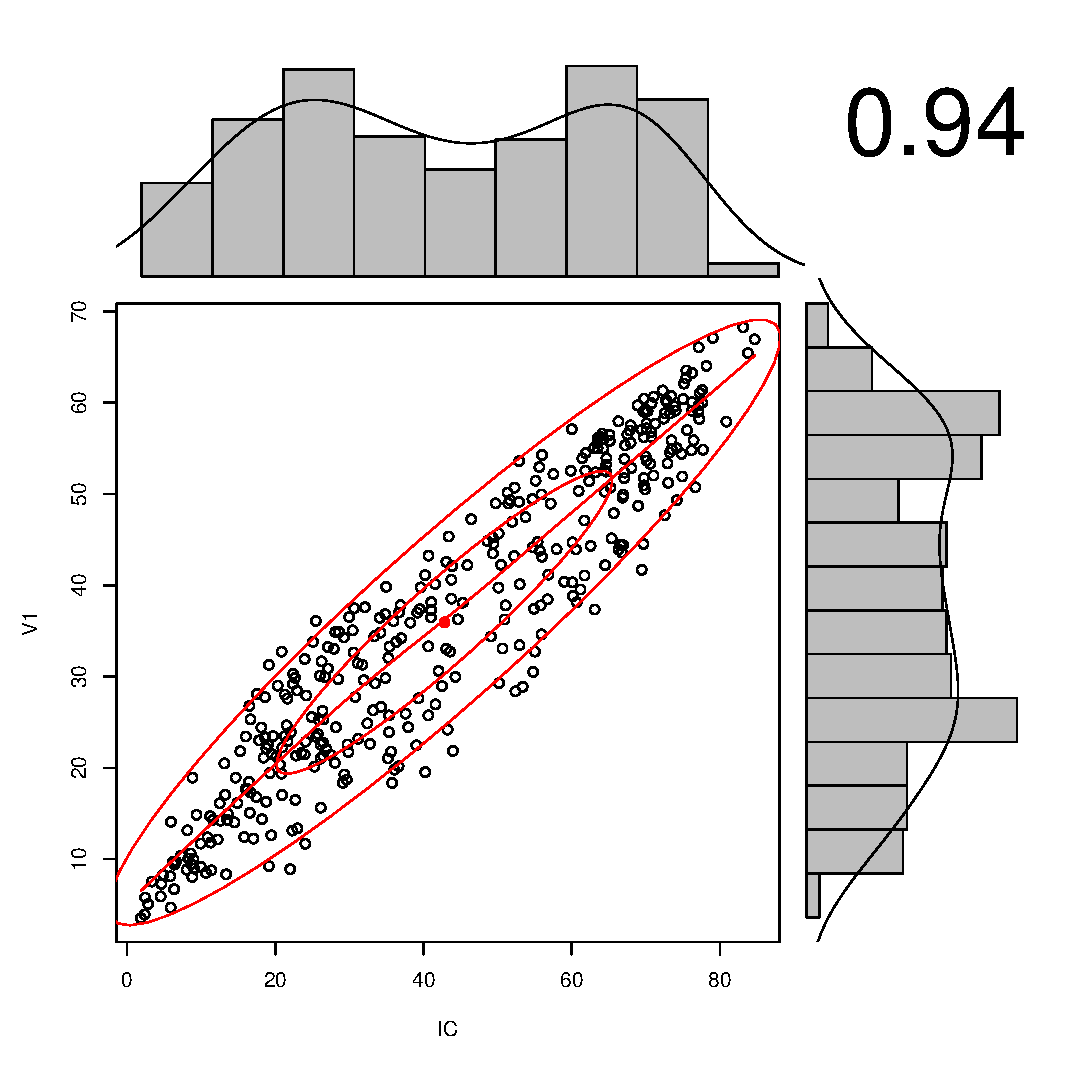
\includegraphics[height=5cm,width=6cm]{figures/HIST_ENxIC.eps}
%DIF < \caption{Scatterplot of the wind capacity factor with EN and IC time series. Histograms and inconditional correlation between these two time series are also provided.}
%DIF < \label{scat_ENIC}
%DIF < \end{figure}
%DIF < 
%DIF < \begin{figure}[htbp]
%DIF < \centering
%DIF < 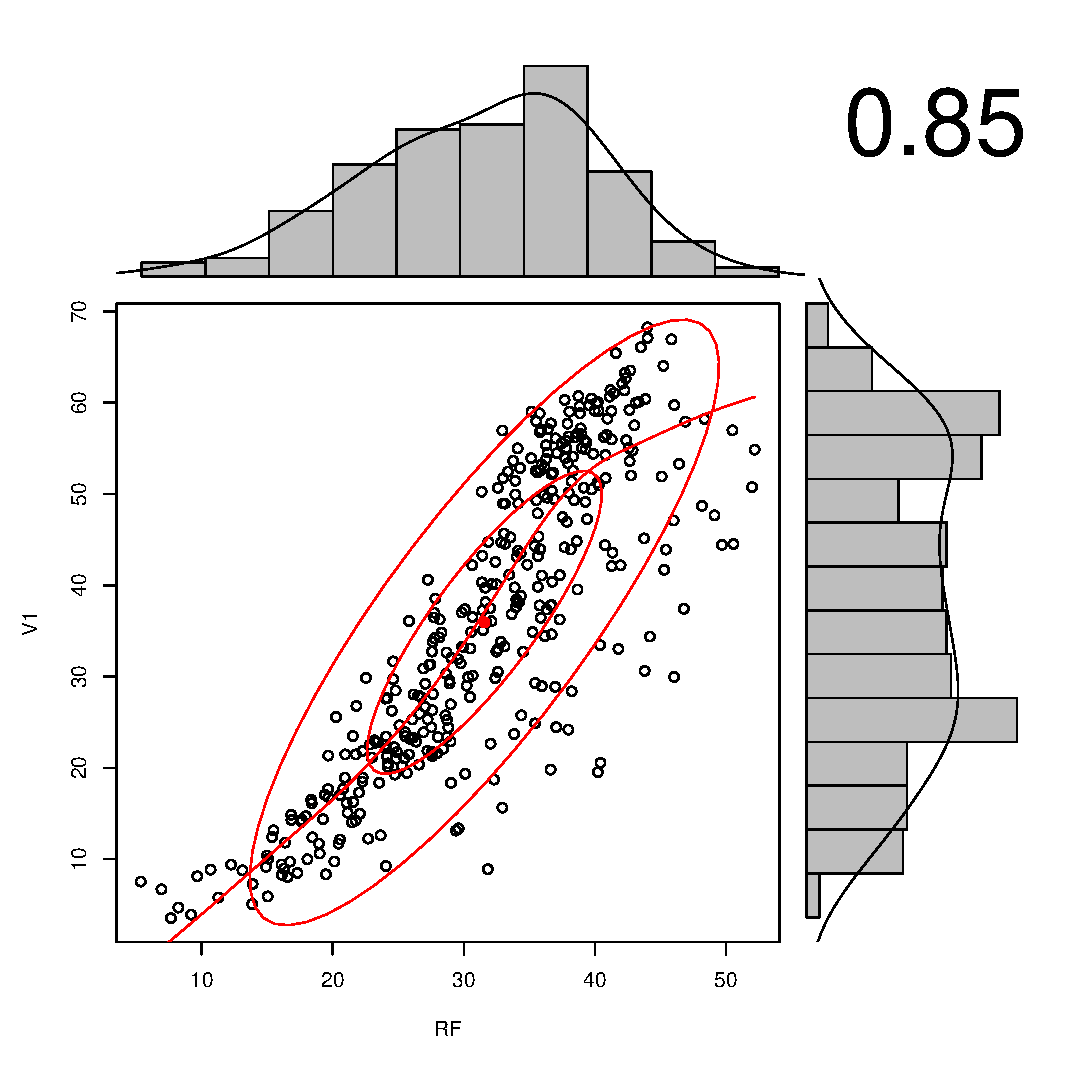
\includegraphics[height=5cm,width=6cm]{figures/HIST_RFxEN.eps}
%DIF < \caption{Scatterplot of the wind capacity factor with RF and EN time series. Histograms and inconditional correlation between these two time series are also provided.}
%DIF < \label{scat_RFEN}
%DIF < \end{figure}
%DIF < 
%DIF < \begin{figure}[htbp]
%DIF < \centering
%DIF < 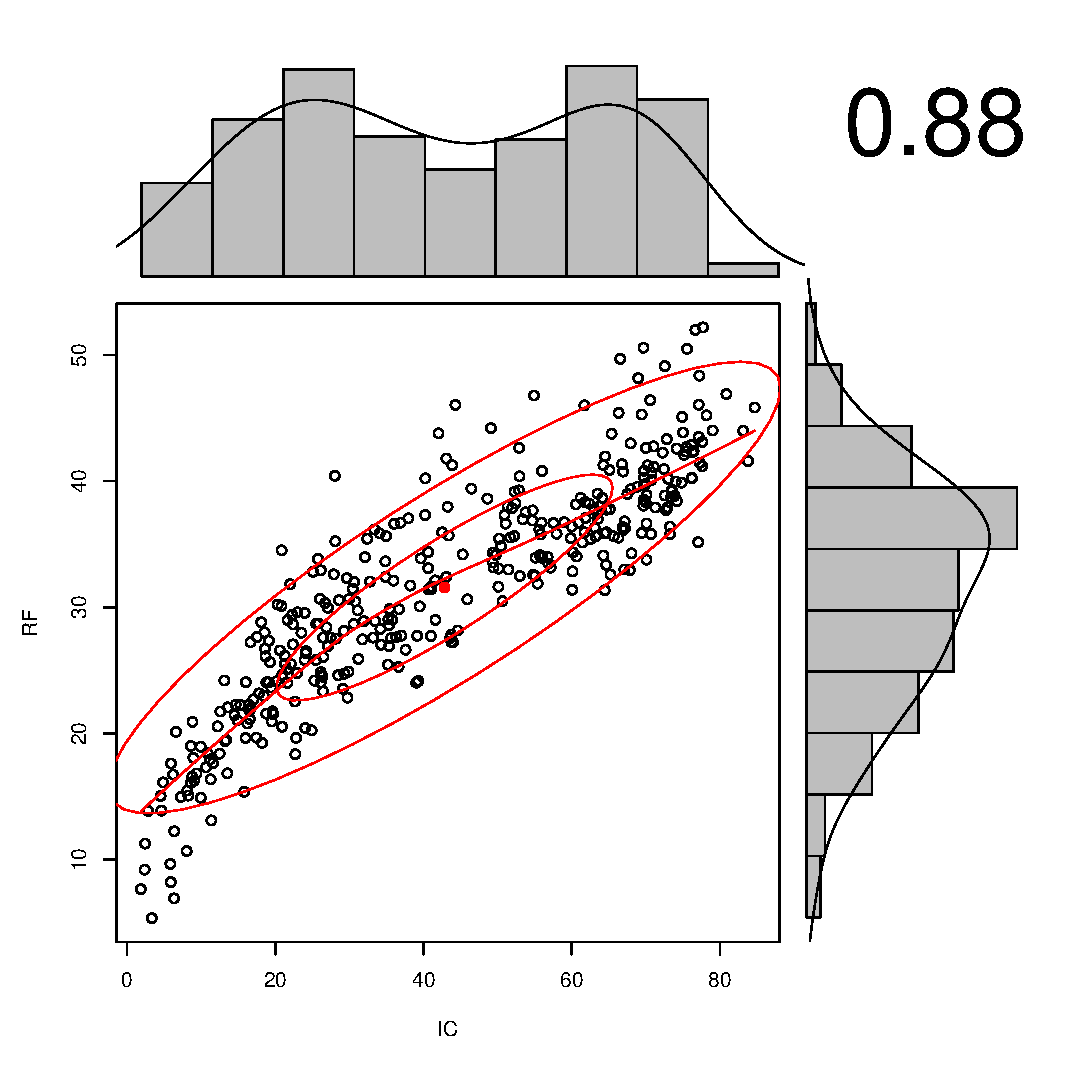
\includegraphics[height=5cm,width=6cm]{figures/HIST_RFxIC.eps}
%DIF < \caption{Scatterplot of the wind capacity factor with RF and IC time series. Histograms and inconditional correlation between these two time series are also provided.}
%DIF < \label{scat_RFIC}
%DIF < \end{figure}
%DIF < 
%DIFDELCMD < 

%DIFDELCMD < %%%
%DIF < A general framework for the specification of feasible time series models Such framework has be recently proposedThe score driven, known as Generalized Autoregressive Score (GAS) model, is an observation-driven model that allows parameters to change over time, having the score as its main driving force \cite{creal2013generalized}. Stacionarity and ergodicity properties of such models shall not be discussed in this paper, nevertheless it were already proven in \cite{blasques2014stationarity}.
%DIFDELCMD < 

%DIFDELCMD < %%%
%DIF < In spite of most of the final users having interest in the capacity factor (CF\footnote{Capacity factor is an average power generated over a period of time, divided by the maximum power of the wind turbine}) as the final outcome variable, the majority of the proposed methodologies in the literature  are mainly concerned in converting wind speed density forecasts to wind power density forecasts through the power curve. With these results in hands, it is then possible to calculate the CF of the former wind turbine.
%DIFDELCMD < 

%DIFDELCMD < %%%
%DIF < In our problem set we have several wind plants from which one needs to generate joint scenarios for CF. The need for such scenarios can arise in many practical problems. For example, such scenarios can be used as input for regulatory purposes, such as the study of a new method to calculate firm energy certificates for wind plants, and also for commercialization strategies firmed at the Free Trade Environment (FTE). Such environment is part of the Brazilian electricity market where investors are able to buy contracts associated with wind plants thorough an auction system (see \cite{barroso2011offering} and references therein). It is then natural in such a decision process to evaluate the risk associated with contracts acquired to buy future energy that will be provided by a portfolio of wind plants. For evaluation purpose it is then necessary to jointly simulate capacity factor for wind plants.
%DIFDELCMD < 

%DIFDELCMD <  %%%
%DIF < Additionally, GAS models are suitable to model non-linear and non-stationary time-series which are also features of wind speed and wind power time series. 
%DIFDELCMD < 

%DIFDELCMD < %%%
%DIF < The parametric assumption is, somehow, important. Since the distribution shape only depends on a few parameters, when dealing with parametric approaches, the computational burden reduces \cite{zhang2014review}. Nevertheless, it is not reasonable to assume that wind power predictive density shape will not vary over time, due to its strong seasonal pattern. However, it is very complex to deal with multi-modal distributions, therefore non-parametric approaches figures as feasible alternatives, but computationally expensive.
%DIF < We develop a model that lies inside the parametric approach to represent the wind power generation and does not need to transform variables.
%DIF < 
%DIFDELCMD < 

%DIFDELCMD < %%%
%DIF < Indeed methods for wind power density forecasting are much less developed. The most direct approach to fulfill such task is proposing a time series model for the marginal densities, but due to the non-linearity of wind power it is not that simple. Therefore, the former reason justifies the use of the power curve to relate wind power and wind speed densities forecasting. To represent wind power uncertainty, one could use probabilistic forecasting \cite{bremnes2004probabilistic}, risk index \cite{pinson2004line} and scenario forecasting \cite{pinson2009probabilistic}. 
%DIFDELCMD < 

%DIFDELCMD < %%%
%DIF < Given the empirical evidence of positive correlation between the time series of CF's, it is crucial to incorporate such information when generating the joint scenarios. More commonly, such dependence is usually captured by estimating a covariance matrix $\Sigma$ \cite{pinson2009probabilistic}.  For example, \cite{morales2010methodology} uses a multivariate ARMA model and employed the variance-covariance matrix to characterize the spatial-temporal correlation of wind speed distribution. Under the multivariate assumption, a Vector Autoregressive Moving Average-GARCH model was employed to describe the bivariate wind vector time-series \cite{jeon2012using}. 
%DIF < 
%DIF < The generation of joint scenarios for a vector of time series is accomplished by use of a multivariate time series model, as for example, a vector auto regression (VAR) under the assumption of a multivariate conditional Gaussian distribution. In this paper, instead of specifying such a distribution from the outset, the multivariate distribution will be constructed by joining the marginal distributions associated with each individual time series via a copula. The use of copulas will make it possible to capture dependence, possibly non-linear, among the time series of CF's associated with plants in different geographical sites.
%DIF < 
%DIF < In our work, the dependence structure among the time series of wind plants is captured through a Student t copula with time-varying correlation matrix \cite{creal2011dynamic} and fixed degrees of freedom. Copula-based models are very flexible  to construct multivariate distributions, since they allow the specification of the models for the marginals distributions (in our case the beta GAS models)separately from the dependence structure given by the copula.
%DIF < Details on estimation and inference for copulas applied to time series can be seen in \cite{cherubini2004copula,joe2005asymptotic, patton2012copula, patton2009copula, patton2006modelling, patton2002applications}. The adoption of a time-varying correlation matrix for the copula is justified by the fact that correlation among wind plants time series are not constant over time due to the fact that wind have different regimes depending on seasons. In our set up the correlation matrix will also evolve in time according to an appropriate GAS mechanism, which will makes it easier to capture and correct for outlier effects, as presented in \cite{creal2011dynamic}. %Nevertheless, it does not seems reasonable to assume that the dependence structure among such variables will be constant, therefore we propose a copula model with a time-varying correlation matrix also being update trough a GAS mechanism.
%DIFDELCMD < 

%DIFDELCMD < %%%
%DIF < In addition, as already mentioned in the introduction, when dealing with a decision-making problem, it seems more reasonable to use probability forecast which can provide a whole new set of quantitative information. In this sense it is commonly used, to reproduce such uncertainty, a Probability Density Function (PDFs) or a Cumulative Distribution Function (CDFs). Furthermore, it was proposed in the literature the use of Kernel Density Estimator (KDE) \cite{bessa2012time} and Quantile Regression (QR) \cite{bremnes2004probabilistic}.% Nevertheless, KDE suffer from the boundary effect problem \cite{wand1994kernel} and QR from the crossing-quantiles one [???]. In spite of having overcome such issues proposing new methodologies XX XX XX XX.
%DIFDELCMD < 

%DIFDELCMD < %%%
%DIF < The literature on the joint generation of capacity factors in Brazil has the VARX model for the vector of log of capacity factors as its benchmark. See, for example, \cite{FosteringWPP}. However, given the Gaussianity assumption of VARX models, it is necessary to exponentiate the simulated values in order to avoid the possibility of generating negative capacity factors. Unfortunately this strategy can produce disproportionally high levels for the simulated capacity factors, rendering unrealistic inputs for estimating risk.
%DIFDELCMD < 

%DIFDELCMD < %%%
%DIF < In the sequel we first discuss how univariate GAS models and a elliptical copula model can be combined to jointly simulate wind CF scenarios, Section \ref{marginals} and Section \ref{copula}. Then we present a method that combines the information from the copula model into the marginal densities to generate a multivariate joint density of CF. To motivate the use of our proposed methodology, we generate wind CF scenarios of three wind plants located at the Northest of Brazil.%run a case study supposing a portfolio of contracts from three Brazilian wind plants and evaluate its risk, considering scenarios with dependence structure and without it.
%DIFDELCMD < 

%DIFDELCMD < %%%
\DIFdelend % ========== ========== ========== ========== ========== 
% ===== Sec. II - Marginal Models ===== %
% ========== ========== ========== ========== ========== 

\section{\DIFdelbegin \DIFdel{Score driven }\DIFdelend \DIFaddbegin \DIFadd{GAS }\DIFaddend models} \label{marginals}

\DIFdelbegin \DIFdel{Our time series data comprises of monthly measures of wind capacity factors (CF), which can only assume values }\DIFdelend \DIFaddbegin \DIFadd{We consider a generic normalized WPG time series with a support }\DIFaddend in the range [0,100), \DIFdelbegin \DIFdel{indicating at the outset, the non adequacy of models with Gaussian distribution. In addition, such time series display a strong seasonal pattern derived from the inter annual variation of wind speed. These data features suggest that a proper model for CF series has to be non Gaussian with parameters that change in time, so that short term and seasonal variations can be properly captured. Firstly, one should choose an adequate density to each of the wind CF timeseries. %DIF < one should look for densities in which the time series values are contained into the densities support range.
After trying several non Gaussian densities the best candidate was the beta}\DIFdelend \DIFaddbegin \DIFadd{in percentage of the maximum power injected. The densities selection rely on the support range and shape of conditional distributions. In this work we select and study the case of a Beta distribution with the first-shape parameter varying over time}\DIFaddend . More precisely, in our application\DIFdelbegin \DIFdel{the CF time series $y_t$ is properly }\DIFdelend \DIFaddbegin \DIFadd{, the $i$-th, from a set of $K$, WPG time series is }\DIFaddend described by a beta \DIFdelbegin \DIFdel{density as follows,
%DIF < from January 1981 to December 2011, measured at three wind plants located in the Brazilian Northeast, namely: Rio do Fogo (RF), Icaraizinho (IC) and Enacel (EN).  Since CF´s have nominal support in $[0,100)$, we propose a beta density function with support in $[0,m)$, as the univariate model for each CF, with m to be specified. Then, each marginal model will be specified as follows
}\begin{align*}\DIFdel{
p(y_{it}|f_{it},\mathcal{F}_{t-1};\theta) \sim Beta\left(\beta_{it},\alpha_{i}\right),\,\,\forall\,\, i \in I \,\, \mbox{and}\,\, t \in T, \label{beta_dens}
}\end{align*}
%DIFAUXCMD
\DIFdelend \DIFaddbegin \DIFadd{probability density function (PDF) as follows:
}

\begin{equation}\DIFadd{
p(y_{it}|f_{it},\mathcal{F}_{i,t-1};\theta_i) \sim beta\left(\beta_{it},\alpha_{i}\right) \forall\,\, i \in K \,\, \mbox{and}\,\, t \in T, \label{beta_dens}
}\end{equation}

\DIFaddend \noindent
where $y_{it}$ is the \DIFdelbegin \DIFdel{wind CF of the wind plant $i$ }\DIFdelend \DIFaddbegin \DIFadd{WPG injected by unit $i\in K$, }\DIFaddend at time $t$, \DIFdelbegin \DIFdel{$\beta_{it}=h(f_{it})$}\DIFdelend \DIFaddbegin \DIFadd{$f_{it}$ is generally defined as a logarithmic transformation of the time-varying first shape parameter of the beta distribution}\DIFaddend , \DIFdelbegin \DIFdel{$\alpha_i>0$, with $h(\cdot)$ to be chosen.
}%DIFDELCMD < 

%DIFDELCMD < %%%
\DIFdel{To fully specify a GAS model one has to choose which parameters of the distribution will evolve in time and those that will }\DIFdelend \DIFaddbegin \DIFadd{$\beta_{it}$, to avoid nonnegativity constraints in the estimation process, and $\alpha_i$ is the second shape parameter, in this paper assumed to }\DIFaddend be fixed. \DIFdelbegin \DIFdel{The time varying parameters will then follow a GAS(p,q) updating mechanism. Considering the seasonal pattern of CF time series the appropriate form for this mechanism will be given by:
}\begin{displaymath}\DIFdel{
\begin{split}
f_{i,t+1}=\omega_{i}}&\DIFdel{+A_{i,1}s_{i,t}+A_{i,2}s_{i,t-1}+A_{i,3}s_{i,t-2}}\\
&\DIFdel{+A_{i,11}s_{i,t-10}+A_{i,12}s_{i,t-11}}\\
&\DIFdel{+B_{i,1}f_{i,t}+B_{i,2}f_{i,t-1}+B_{i,3}f_{i,t-2}}\\
&\DIFdel{+B_{i,11}f_{ti,-10}+B_{i,12}f_{i,t-11}\label{eq:2}
\end{split}
}\end{displaymath}
%DIFAUXCMD
\DIFdelend \DIFaddbegin \DIFadd{$\theta$ is the vector of hyperparameters, assumed to be static in time, encompassing $\alpha_i$, dummy variables to capture the effect of outliers when needed, and the rest of parameters to be estimated.
}

\DIFadd{Thus, the time-varying parameter GAS$(p,q)$ updating mechanism is devised for $f_{it}$ as follows:
}

\vspace{-0.3cm}
\begin{equation}\DIFadd{
{f}}\DIFadd{_{i,t+1} = \omega_i + \sum_{l=1}^{p} A_{i,l}s_{i,t-l+1} + \sum_{l=1}^{q} B_{i,l}f_{i,t-l+1}. \label{eq:2}
}\end{equation}

\DIFaddend \noindent
\DIFdelbegin \DIFdel{where $f_{i,t}$ is the timevarying parameter of the beta density of the wind plant $i$ at time $t$, $s_{i,t}$ }\DIFdelend \DIFaddbegin \DIFadd{In expression }\eqref{eq:2}\DIFadd{, $s_{i,t-l+1}$ }\DIFaddend is the score of the beta \DIFdelbegin \DIFdel{density of the wind plant }\DIFdelend \DIFaddbegin \DIFadd{PDF for unit }\DIFaddend $i$ at time \DIFdelbegin \DIFdel{$t$ and the $\omega$'s, $A$'s and $B$'s }\DIFdelend \DIFaddbegin \DIFadd{$t-l+1$, and $\omega_i$, $A_{i,l}$, and $B_{i,l}$ }\DIFaddend are fixed parameters\DIFdelbegin \DIFdel{which will be estimated by maximum likelihood. }\DIFdelend \DIFaddbegin \DIFadd{, which are considered as part of vector $\theta_i$. %DIF > Thus, in this work, $\theta = [\textbf{A}_i,\textbf{B}_i,\omega_i]^T$, where $\textbf{A}_i$ and $\textbf{B}_i$ stand for the vector contain all lags of $A_{i,l}$ and $B_{i,l}$ fixed parameters.
}\DIFaddend 

To complete the description of the the updating mechanism of GAS models it is necessary to define \DIFdelbegin \DIFdel{$s_{t}$ }\DIFdelend \DIFaddbegin \DIFadd{$s_{i,t}$ }\DIFaddend in  Equation \eqref{eq:2}. The authors in \cite{creal2013generalized} \DIFdelbegin \DIFdel{propose }\DIFdelend \DIFaddbegin \DIFadd{proposed }\DIFaddend the following scheme:
\begin{align}
s\DIFdelbegin \DIFdel{_{t} }\DIFdelend \DIFaddbegin \DIFadd{_{i,t} }\DIFaddend &= \mathcal{I}\DIFdelbegin \DIFdel{_{t|t-1}}\DIFdelend \DIFaddbegin \DIFadd{_{i,t|t-1}}\DIFaddend ^{-d} \cdot \nabla\DIFdelbegin \DIFdel{_{t}}\DIFdelend \DIFaddbegin \DIFadd{_{i,t}}\DIFaddend \label{eq:score1}\\
\nabla\DIFdelbegin \DIFdel{_{t} }\DIFdelend \DIFaddbegin \DIFadd{_{i,t} }\DIFaddend &= \DIFdelbegin \DIFdel{\frac{\partial \ln p(y_{t}|f_{t},\mathcal{F}_{t-1};\theta)}{\partial f_{t}}}\DIFdelend \DIFaddbegin \DIFadd{\frac{\partial \ln p(y_{i,t}|f_{i,t},\mathcal{F}_{i,t-1};\theta_i)}{\partial f_{i,t}}}\DIFaddend \label{eq:score2}\\
\mathcal{I}\DIFdelbegin \DIFdel{_{t|t-1} }\DIFdelend \DIFaddbegin \DIFadd{_{i,t|t-1} }\DIFaddend &= E\DIFdelbegin \DIFdel{_{t|t-1}[\nabla_{t}^T\nabla_{t}]}\DIFdelend \DIFaddbegin \DIFadd{_{t|t-1}[\nabla_{i,t}^{T}\nabla_{i,t}]}\DIFaddend ,\label{eq:score3} 
\end{align}
\noindent
where \DIFdelbegin \DIFdel{$p(y_{t}|f_{t},\mathcal{F}_{t-1};\theta)$ }\DIFdelend \DIFaddbegin \DIFadd{$p(y_{i,t}|f_{i,t},\mathcal{F}_{i,t-1};\theta_i)$ }\DIFaddend is the observation \DIFdelbegin \DIFdel{density function, $\mathcal{F}_{t-1}$ }\DIFdelend \DIFaddbegin \DIFadd{PDF, $\mathcal{F}_{i,t-1}$ }\DIFaddend collects all relevant information \DIFaddbegin \DIFadd{of time series $i$ }\DIFaddend up to time $t-1$, and \DIFdelbegin \DIFdel{$\mathcal{I}_{t|t-1}$ }\DIFdelend \DIFaddbegin \DIFadd{$\mathcal{I}_{i,t|t-1}$ }\DIFaddend is a scaling \DIFdelbegin \DIFdel{matrix with appropriate dimensions. Different choices of $d$ results in different GAS models: $d=1$ means that it will be use the inverse of Fisher Information matrix, $d=1/2$ the pseudo-inverse of Fisher Information matrix $d=0$ the identity matrix}\DIFdelend \DIFaddbegin \DIFadd{factor, which accounts for the variance of $s_{i,t}$}\DIFaddend . More details can be found in \cite{creal2013generalized}. In practice, the choice of $d$ has shown to be an empirical question: for a given model one chooses the value of $d$ which produces best diagnostics and forecasting.

\DIFdelbegin \subsection{\DIFdel{Parametrization}}
%DIFAUXCMD
\addtocounter{subsection}{-1}%DIFAUXCMD
%DIFDELCMD < 

%DIFDELCMD < %%%
\DIFdel{Having in mind that the first shape parameter of the beta density, $\beta_{t}>0$}\DIFdelend \DIFaddbegin \DIFadd{As mentioned before, because the beta parameter can only assume positive values}\DIFaddend , it is \DIFdelbegin \DIFdel{natural to choose $\beta_{t}=exp\{f_{t}\}$. From this, it follows that Equations }%DIFDELCMD < \eqref{beta_dens}%%%
\DIFdel{-}%DIFDELCMD < \eqref{eq:score3} %%%
\DIFdel{should also be re-parametrized with regard to $\ln(\beta_t)$. Considering a monotonically increasing mapping function $h(\cdot)$, then $\tilde{f}_{t}=h(f_{t})$. Taking $\dot{h_{t}} = \partial h(f_{t})/f_{t}^{'}$, the beta GAS specification updating mechanism, will be
}\begin{align*}\DIFdel{
\dot{h}_{t} }&\DIFdel{= \frac{1}{\beta_{t}}\nonumber}\\
\DIFdel{\tilde{\nabla_{t}}}&\DIFdel{=\beta_{t}\left\{\ln y_{t} - }[\DIFdel{\ln k + \psi_{1}(\beta_{t}) - \psi_{1}(\beta_{t}+\alpha)}]\DIFdel{\right\}}\\ \DIFdel{\nonumber
\tilde{\mathcal{I}}_{t|t-1} }&\DIFdel{= \left\{ \beta_{t}^{2} }[ \DIFdel{\psi_{2} (\beta_{t} + \alpha) - \psi_{2} (\beta) }] \DIFdel{\right\}^{-1}}\\
\DIFdel{\tilde{s}_{t}}&\DIFdel{=\frac{\ln y_{t} - [\ln k + \psi_{1}(\beta_{t}) - \psi_{1}(\beta_{t}+\alpha)]}{\beta_{t}^{1-2d}[\psi_{2}(\beta_{t}) - \psi_{2}(\beta_{t} + \alpha)]^{1-d}},\label{betascore1}
}\end{align*}
%DIFAUXCMD
\DIFdelend \DIFaddbegin \DIFadd{conveniently reparameterized as the exponential of an unconstrained parameter, namely, $f_{i,t}$. In addition, to remove the effect of possible outliers, dummy variables can be considered into parametrization. In this sense, if we define the time-varying beta parameter as 
}\begin{equation}\DIFadd{
\beta_{i,t} = e^{\phi_i^T D_{i,t} + f_{i,t}}, \label{eq:exogena}
}\end{equation}

\DIFaddend \noindent
\DIFdelbegin \DIFdel{where $\psi_{i}$ stands for the $i$-th order derivative of the logarithm of the gamma function.
}\DIFdelend \DIFaddbegin \DIFadd{with
}\begin{equation}\DIFadd{
D_{i,t}=
\begin{cases}
1 , }& \DIFadd{\text{if } y_{i,t} \text{ is an outlier;} }\\
\DIFadd{0,  }& \DIFadd{\text{otherwise}.
\end{cases}
}\end{equation}
\DIFaddend 

\DIFdelbegin \subsection{\DIFdel{Initial values}}
%DIFAUXCMD
\addtocounter{subsection}{-1}%DIFAUXCMD
\DIFdelend \DIFaddbegin \subsection{\DIFadd{Estimation}} \label{MVunivariado}
\DIFaddend 

\DIFdelbegin \DIFdel{In practice, to initialize recursion }\DIFdelend \DIFaddbegin \DIFadd{Regarding the estimation of the fixed parameter vector $\theta_i$ for each time series $i$, the estimation procedure is based on the following log-likelihood maximization problem:%DIF > \footnote{We recall that the first shape parameter of the beta density, $\beta_{i,t}$, can be recovered after the estimation process by making $\beta_{i,t}=exp\{f_{i,t}\}$.}: 
}

\begin{equation}\DIFadd{
\hat{\theta}_i = arg\underset{\theta_i}{max} \sum_{t=1}^{n} ln}[\DIFadd{p(y_{i,t}|f_{i,t},\mathcal{F}_{i,t-1};\theta_i)}]\DIFadd{.\label{eq:max}
}\end{equation}

%DIF > From this, it follows that Equations \eqref{beta_dens}-\eqref{eq:score3} should also be re-parametrized with regard to $\ln(\beta_t)$. Considering a monotonically increasing mapping function $h(\cdot)$, then $\tilde{f}_{t}=h(f_{t})$. Taking $\dot{h_{t}} = \partial h(f_{t})/f_{t}^{'}$, the beta GAS specification updating mechanism, will be
%DIF > \begin{align}
%DIF > \dot{h}_{t} &= \frac{1}{\beta_{t}}\nonumber\\
%DIF > \tilde{\nabla_{t}}&=\beta_{t}\left\{\ln y_{t} - [\ln k + \psi_{1}(\beta_{t}) - \psi_{1}(\beta_{t}+\alpha)]\right\}\\
%DIF > \tilde{\mathcal{I}}_{t|t-1} &= \left\{ \beta_{t}^{2} [ \psi_{2} (\beta_{t} + \alpha) - \psi_{2} (\beta) ] \right\}^{-1}\\
%DIF > \tilde{s}_{t}&=\frac{\ln y_{t} - [\ln k + \psi_{1}(\beta_{t}) - \psi_{1}(\beta_{t}+\alpha)]}{\beta_{t}^{1-2d}[\psi_{2}(\beta_{t}) - \psi_{2}(\beta_{t} + \alpha)]^{1-d}},\label{betascore1}
%DIF > \end{align}
%DIF > \noindent
%DIF > where $\psi_{i}$ stands for the $i$-th order derivative of the logarithm of the gamma function.

\DIFadd{Because $f_{i,t}$ is a function of $\theta_i$ (we recall that the coefficients in equation }\DIFaddend \eqref{eq:2} \DIFdelbegin \DIFdel{at $t=1$, it is necessary to have lagged values of the time varying parameter $f_{t}$. As $s_{t}$ is a direct function of $f_{t}$, it is straightforward to calculate its lagged values. Then we will concentrate on deriving lagged values for $f_{t}$. Denote the initial time varying parameters values as $f_{i,1-q}=\{f_{i,0},f_{i,-1},...,f_{i,1-q}\}$, where $q$ denotes the persistence of the value $f_{t}$ over time, as shown by equation }%DIFDELCMD < \eqref{eq:2}%%%
\DIFdel{. In our particular case, the wind CF }\DIFdelend \DIFaddbegin \DIFadd{are all part of the vector of hyperparameters, $\theta_i$), to solve the estimation problem }\eqref{eq:max}\DIFadd{, a numerical non-linear optimization procedure has to be used. In this work, we apply the Nelder Mead algorithm to find good initial points to the BFGS algorithm. Notwithstanding, the evaluation of the log-likelihood function requires initial values for $f_{i,0},f_{i,-1},...,f_{i,1-q}$ and $s_{i,0},s_{i,-1},...,s_{i,1-p}$. These  are obtained by fitting fixed beta distributions, one for each month, assuming both parameters fixed in time. More precisely, the WPG }\DIFaddend time series is split into 12 monthly time series, i.e., $\{Y_{Jan}^{(i)},..., Y_{Dec}^{(i)}\}$. \DIFdelbegin \DIFdel{For }\DIFdelend \DIFaddbegin \DIFadd{Then, for }\DIFaddend each of these time series \DIFdelbegin \DIFdel{$\{Y_{m}^{(i)}\}_{m=1}^{12}$, estimate via maximum likelihood the static shape parameters of a beta density, $\alpha_{i}$ and $\beta_{i}$. Then use these estimates to initialize Equation }\DIFdelend \DIFaddbegin \DIFadd{$\{Y_{v}^{(i)}\}_{v=1}^{12}$, a fixed beta density is estimated  via maximum likelihood, resulting in the estimates  $\{\alpha_{v}^{(i)}\}_{v=1}^{12}$ and $\{\beta_{v}^{(i)}\}_{v=1}^{12}$. These are then used to initialize the recursion in }\DIFaddend \eqref{eq:2} \DIFdelbegin \DIFdel{, having in mind the new parametrization, $f_{i,t}=\ln(\beta_{i,t})$. Note that using this methodology, the first twelve observations of the time series are removed in order to estimate the initial values of the time varying parameter of the beta density. As a result, the maximum likelihood and the residuals of }\DIFdelend \DIFaddbegin \DIFadd{for each evaluation of the log-likelihood function. Thus, the function that is passed to }\DIFaddend the \DIFdelbegin \DIFdel{beta GAS(p,q) model are only computed after the thirteenth observation}\DIFdelend \DIFaddbegin \DIFadd{BFGS algorithm is a numerical function that receives as input a trial value for vector $\theta_i$, calculates the value of $f_{i,t}$ according to expression }\eqref{eq:2}\DIFadd{, and returns as output the value of expression }\eqref{eq:max}\DIFadd{. Based on an initial value for $\theta_i$, the BFGS algorithm iterates until finding a local maximum point. To enhance the solution quality, a Nelder Mead algorithm is used on the top of this process and its solution is used as initial points for the BFGS step and it iterates until the GAP between theses solutions are smaller than 0.1}\DIFaddend .

\subsection{Diagnostics}

\DIFdelbegin \DIFdel{In GAS models diagnostics can be evaluated }\DIFdelend \DIFaddbegin \DIFadd{Diagnostics in GAS models can be obtained }\DIFaddend using an appropriate type of residuals for non linear \DIFdelbegin \DIFdel{/ }\DIFdelend \DIFaddbegin \DIFadd{and }\DIFaddend non Gaussian time series models known as quantile residuals. As described in \cite{dunn1996randomized}, the observed quantile residual is given by
\DIFdelbegin \begin{align*}\DIFdel{ \label{residq}
r_{t,\hat{\theta}} = \Phi^{-1}(F(y_{t}|f_{t},\mathcal{F}_{t},\hat{\theta})).
}\end{align*} 
 %DIFAUXCMD
\DIFdelend \DIFaddbegin \begin{equation}\DIFadd{ \label{residq}
r_{t,\hat{\theta}_i} = \Phi^{-1}[F(y_{i,t}|f_{i,t},\mathcal{F}_{i,t-1};\hat{\theta}_i)].
}\end{equation} 
\DIFaddend 

\DIFdelbegin \DIFdel{where }\DIFdelend \DIFaddbegin \DIFadd{Where }\DIFaddend $F(\cdot)$ is the \DIFdelbegin \DIFdel{CDF associated with $p(y_{t}|f_{t},\mathcal{F}_{t-1};\theta)$ and $\Phi^{-1}$ }\DIFdelend \DIFaddbegin \DIFadd{cumulative distribution function (CDF) associated with the proposed beta density  $p(y_{i,t}|f_{i,t},\mathcal{F}_{i,t-1};\theta_i)$ and $\Phi^{-1}[\cdot]$ }\DIFaddend is the quantile \DIFaddbegin \DIFadd{function }\DIFaddend of a standard Gaussian distribution. Under correct model specification\DIFaddbegin \DIFadd{, }\DIFaddend these residuals should be normally distributed and show no \DIFaddbegin \DIFadd{temporal }\DIFaddend dependence. These can be checked, for example, using the Jarque Bera test for normality, \DIFdelbegin \DIFdel{and }\DIFdelend the Ljung Box test for absence of serial correlation\DIFaddbegin \DIFadd{, }\DIFaddend and Ljung Box (on squared residuals) to test for absence of \DIFaddbegin \DIFadd{non linear dependence, such as }\DIFaddend ARCH effect. 

\DIFdelbegin \subsection{\DIFdel{Univariate Forecasting}}
%DIFAUXCMD
\addtocounter{subsection}{-1}%DIFAUXCMD
%DIFDELCMD < 

%DIFDELCMD < %%%
\DIFdel{The $k$ steps ahead distribution conditional on observations up to time $t$, $p(y_{t+k}|\mathcal{F}_{t} )$, is only analytical for $k=1$, when it coincides with the chosen probability model. However, for $k>1$ it has to be evaluated using Monte Carlo simulation.
}\DIFdelend %DIF > \subsection{Univariate Forecasting}
%DIF > 
%DIF > The $h$ steps ahead distribution conditional on observations up to time $t$, $p(y_{i,t+h}|\mathcal{F}_{i,t} )$, is only analytic for $h=1$, when it coincides with the chosen probability model. For more than one step ahead, $h>1$, it has to be evaluated using Monte Carlo simulation.


% ===== Sec. III - Copula Model ===== %

\section{\DIFaddbegin \DIFadd{Spatial }\DIFaddend Dependence model}\label{copula}

\DIFdelbegin \DIFdel{In the previously section, non Gaussian time series models were proposed to model }\DIFdelend \DIFaddbegin \DIFadd{Once the proposed beta GAS models were individually applied to }\DIFaddend each of the \DIFdelbegin \DIFdel{wind CF time series. To derive a proper mechanism for joint scenario generation of CF's time seriesit is also necessary to capture }\DIFdelend \DIFaddbegin \DIFadd{$K$ WPG time series, }\DIFaddend the observed dependence among \DIFdelbegin \DIFdel{the CF's time series. For this conditional copula models introduced by \mbox{%DIFAUXCMD
\cite{patton2002applications}
}%DIFAUXCMD
are used. %DIF < In the following, the same author addressed the possibility of modeling the correlations among two random variables as a time varying process \cite{patton2006modelling}. Additionally, in the former work, the author boosted the driving mechanism to a generally applicable driving mechanism for copula parameters. Further multivariate extensions were presented in \cite{patton2009copula} and \cite{patton2012copula}.
}%DIFDELCMD < 

%DIFDELCMD < %%%
\DIFdel{More specifically, using the framework developed in \mbox{%DIFAUXCMD
\cite{patton2012copula}
}%DIFAUXCMD
, it will be possible to allow the correlations between pairs of CF's time series to change in time according to a GAS mechanism that will be described in the sequel. As it will be seen, it is straightforward to combine marginal densities as given by GAS models with copulas that also have time varying parameters. %DIF < If we assume that, when we simulate the joint values, the correlation among those plants shall be taken as a static value all over the forecasting horizon. Therefore we will address the possibility of modeling the observed dependency among the wind plants as a time-varying process. Nevertheless, to update such time varying process we use the same GAS mechanism formerly presented in Section \ref{marginals}. 
}%DIFDELCMD < 

%DIFDELCMD <  %%%
\DIFdel{Considering each of the time series models $y_{it}$ estimated individually using a GAS model, $u_{it}$ denotes }\DIFdelend \DIFaddbegin \DIFadd{different units is captured by }\DIFaddend the probability integral \DIFdelbegin \DIFdel{transform }\DIFdelend \DIFaddbegin \DIFadd{transformed }\DIFaddend (PIT) \DIFdelbegin \DIFdel{variable obtained from the marginal beta GAS(p, q) model described in section \ref{marginals}. That is 
}\DIFdelend \DIFaddbegin \DIFadd{variables, $\mathbf{u}_{t} \in \mathbb{R}^K$, which are calculated as 
}\DIFaddend \begin{eqnarray}\DIFaddbegin \label{pits}
\DIFaddend u\DIFdelbegin \DIFdel{_{it}}\DIFdelend \DIFaddbegin \DIFadd{_{i,t}}\DIFaddend =F\DIFdelbegin \DIFdel{_{beta}}\DIFdelend (y\DIFdelbegin \DIFdel{_{it}}\DIFdelend \DIFaddbegin \DIFadd{_{i,t}}\DIFaddend |f_{i,t},\mathcal{F}\DIFdelbegin \DIFdel{_{i,t}}\DIFdelend \DIFaddbegin \DIFadd{_{i,t-1}}\DIFaddend ,\hat{\theta}_{i}) \,\, \forall \,\,i \in \DIFdelbegin \DIFdel{I}\DIFdelend \DIFaddbegin \DIFadd{K}\DIFaddend \,\, \mbox{and} \,\, t=13,\ldots,T\DIFaddbegin \DIFadd{.
}\DIFaddend \end{eqnarray}
\noindent
\DIFdelbegin \DIFdel{where $\hat{\theta_i}=\{\hat{\alpha} _{i},\hat{\omega} _{i}, \hat{A}_{i}'s, \hat{B}_{i}'s\}\,\,  \forall \,\, i=1,2,3$ is the estimated vector of fixed parameters from the univariate beta models. The driving mechanism presented in \mbox{%DIFAUXCMD
\cite{creal2011dynamic}
}%DIFAUXCMD
, was derived for a multivariate Student t, being the Gaussian density a particular case of this when $\nu^{-1} \to 0$. 
Such density then acts on the $T \times I$ vector $\tilde{y}_{t}^{'}=[F_{\nu}^{-1}(u_{1t}), ..., F_{\nu}^{-1}(u_{it})]^{'}$, where $F_{\nu}^{-1}(\cdot)$ is the univariate inverse }\DIFdelend \DIFaddbegin \DIFadd{The PIT multivariate time series denoted by $\mathbf{u}_{t}$ belong to the $[0,1]$ support. 
}

%DIF > where $\hat{\theta_i}$ are the estimated fixed parameter vectors from each of the univariate beta GAS model. Due to initial values of the beta GAS models, $t$ starts at 13.After obtaining vector $\mathbf{u}_{t} \in \mathbb{R}^K$, the second step GAS procedure, which updates the time-varying correlation matrix $\Sigma_t$ of the residuals of the beta models, can be estimated.

\DIFadd{Assuming $G_{\nu}$ as the CDF of a univariate }\DIFaddend Student t distribution with $\nu$ degrees of freedom\DIFdelbegin \DIFdel{. The updating of }\DIFdelend \DIFaddbegin \DIFadd{, a new vector of t-Student-distributed time series can be build as follows: $\tilde{y}_{t}=[G_{\nu}^{-1}(u_{1,t}), ..., G_{\nu}^{-1}(u_{K,t})]^T$. The elliptical copula used in this work is developed under the assumption that the transformed time series, $\{\tilde{y}_{t}\}_{t\in T}$, can be modeled as a multivariate t-Student PDF given by:
}

\begin{align}\DIFadd{ 
\begin{split}
g(\tilde{y}_{t}|\Sigma_{t}; \nu) = \frac{\Gamma\left(\frac{\nu+K}{2}\right)}{\Gamma\left(\frac{\nu}{2}\right) [(\nu-2)\pi]^{K/2} |\Sigma_{t}|^{1/2}} \left[ 1+ \frac{\tilde{y}_{t}^{'}\Sigma_{t}^{-1}\tilde{y}_{t}}{(\nu-2)} \right], \label{eq:denstmulti}
\end{split} 
}\end{align}
\noindent
\DIFadd{where $\Sigma_t$ is }\DIFaddend the correlation matrix \DIFdelbegin \DIFdel{through a GAS mechanism follows a similar idea from the dynamical conditional correlation (DCC) model proposed by \mbox{%DIFAUXCMD
\cite{engle2002dynamic}
}%DIFAUXCMD
, and commonly used in Finance. The updating mechanism of the time-varying parameter vector, proposed for this particular density in \mbox{%DIFAUXCMD
\cite{creal2011dynamic}
}%DIFAUXCMD
, is $f_{t}=vech(Q_{t})$, }\DIFdelend \DIFaddbegin \DIFadd{which is assumed to follow a second GAS updating mechanism similar to that proposed in \mbox{%DIFAUXCMD
\cite{engle2002dynamic}
}%DIFAUXCMD
. The key of such model is the use of a factorization scheme for $\Sigma_t$ that allows the updating mechanism to always generate positive definite correlation matrices. Such factorization scheme, used in \mbox{%DIFAUXCMD
\cite{engle2002dynamic}
}%DIFAUXCMD
and simplified here, is described in the sequel: 
}

\begin{align}\DIFadd{
\Sigma_{t} = diag(Q_{t})^{-1/2}Q_{t}diag(Q_{t})^{-1/2}. \label{sigma}
}\end{align}

\noindent
%DIF > In \eqref{sigma}, $D_{t}$ is a diagonal matrix of standard deviations. However regarding the context of this paper, variances are assumed to be known since in a copula specification only the correlations are time-varying, hence $D_{t}=I$, where $I$ is an identity matrix with the appropriate dimensions. 
\DIFaddend where $Q_{t}$ is a symmetric positive definite matrix \DIFdelbegin \DIFdel{, carrying }\DIFdelend \DIFaddbegin \DIFadd{which guarantees a symmetric positive definite matrix $\Sigma_{t}$ with elements outside the main diagonal lying inside the }[\DIFadd{-1,1}] \DIFadd{range.
}

%DIF > and $\Delta_{t}$ is a diagonal matrix which elements are the square root of the elements contained in the main diagonal of $Q_{t}$. The matrix $R_{t}$ applies a parametrization in the matrix $Q_{t}$ which guarantees a symmetric matrix $\Sigma_{t}$, positive definite, with elements outside the main diagonal lying inside [-1,1] range. 

\DIFadd{The matrix $Q_t$ carries }\DIFaddend all the information regarding the \DIFdelbegin \DIFdel{correlation among the wind plants CF's }\DIFdelend \DIFaddbegin \DIFadd{spatial dependence structure among different WPG }\DIFaddend time series. \DIFdelbegin \DIFdel{For details, see \mbox{%DIFAUXCMD
\cite{creal2011dynamic}
}%DIFAUXCMD
. }%DIFDELCMD < {\color{red}%%%
\DIFdel{,
Melhorar essa parte do detalhamento das copulas com GAS }%DIFDELCMD < }
%DIFDELCMD < %%%
\DIFdelend \DIFaddbegin \DIFadd{The idea of adopting a time varying mechanism to update the elements of $Q_t$ is to include the temporal variation of this dependence when generating joint scenarios of WPG. In order to update the quantities of the time-varying vector $q_t=vech(Q_{t})$, which stands for the half-vectorization}\footnote{\DIFadd{The half-vectorization is a linear transformation used to convert the lower triangular portion of $K\times K$ symmetric matrices in to $K(K+1)/2$ vectors.}} \DIFadd{of $Q_{t}$, we adopt the same GAS dynamic proposed in \mbox{%DIFAUXCMD
\cite{creal2011dynamic}
}%DIFAUXCMD
, i.e.,
}\begin{align}\DIFadd{
vech(Q_{t+1}) }&\DIFadd{= \Omega + \Pi s_t + \Upsilon vech(Q_{t}). \label{gasmulti}
}\end{align}
\noindent
\DIFadd{In }\eqref{gasmulti}\DIFadd{, $\Pi$ and $\Upsilon$ are diagonal matrices, $\Omega$ is a $K \times 1$ vector with elements equals to one when updating the elements of the main diagonal of $Q_t$ in order to identify either model. Hence the elements of $\Omega$ corresponding to the diagonal elements of $Q_t$ can be multiplied by any arbitrary positive number without changing the decomposition. Regarding the elements of the GAS mechanism $s_t$, $\nabla_{t}$ and $\mathcal{I}_{t|t-1}^{-1}$ for the multivariate Student t distribution, they were calculated in \mbox{%DIFAUXCMD
\cite{creal2011dynamic}
}%DIFAUXCMD
and can be found in Appendix \ref{FirstAppendix}.
}\DIFaddend 

\subsection{Estimation of the copula parameters}\label{copula_par}
\DIFdelbegin \DIFdel{Estimation of the copula parameters are done using multi-stage optimization approach known as }\DIFdelend \DIFaddbegin \DIFadd{We now deal with the estimation method used in the second-step GAS procedure, i.e., the estimation of the static parameters of the elliptical-copula model, $\Theta=(\nu,\Omega,\Pi,\Upsilon)$. For this we applied the }\DIFaddend Inference for Margins (IFM) \DIFdelbegin \DIFdel{(}\DIFdelend \DIFaddbegin \DIFadd{optimization procedure (see }\DIFaddend \cite{xu1996statistical}, \cite{joe1997multivariate}). In IFM estimation, the \DIFdelbegin \DIFdel{marginal parameters }\DIFdelend \DIFaddbegin \DIFadd{estimated vector of hyperparameters, $\hat{\theta}_i \in K$, of each WPG time series }\DIFaddend are first estimated \DIFdelbegin \DIFdel{, and then conditional on these estimates }\DIFdelend \DIFaddbegin \DIFadd{individually using the same procedure described in Section \ref{MVunivariado}. Then, based on the individual estimates $\hat{\theta}_i \in K$}\DIFaddend , copula parameters are estimated via maximum likelihood. \DIFdelbegin \DIFdel{In IFM estimation the unknown parameter vector is split in two sets, one containing the marginal densities parameters and the other the copula parameters}\DIFdelend \DIFaddbegin \DIFadd{Considering the $K$-dimensional vector $\tilde{y}_{t}=[G_{\nu}^{-1}(u_{1,t}), ..., G_{\nu}^{-1}(u_{K,t})]^T$, the log-likelihood of the multivariate Student t model is
}\begin{equation}\DIFadd{
\begin{split}
\mathcal{L}=}&\DIFadd{\sum_{t=1}^{n}\Bigg\{ log \left[\Gamma \left(\frac{\nu+K}{2} \right) \right] -log \left[\Gamma \left(\frac{\nu}{2} \right) \right]}\\
&\DIFadd{-\frac{1}{2} log |\Sigma_{t}| - \frac{K}{2}log}[\DIFadd{(\nu-2)\pi}] \\&\DIFadd{- \frac{\nu+K}{2} log\left[ 1+\frac{\tilde{y}_{t}^{'}\Sigma^{-1}_{t}\tilde{y}_{t}}{\nu-2}\right] \Bigg\}
\label{VeroT}
\end{split}
}\end{equation}
\noindent
\DIFadd{where the temporal variation of $\Sigma_{t}$ is described by the GAS mechanism provided by Equation }\eqref{gasmulti}\DIFadd{. Maximization of the log-likelihood function $\mathcal{L}$ is analogous to the univariate ones given on Section \ref{MVunivariado}. The estimation problem }\eqref{VeroT} \DIFadd{is solved trough a non-linear optimization procedure which also uses Nelder Mead algorithm to find good initial points to the BFGS algorithm. The degrees of freedom $\nu$ were estimated using profile likelihood. For more details see, \mbox{%DIFAUXCMD
\cite{murphy2000profile}
}%DIFAUXCMD
. %DIF > Regarding initial values for $q_j(j<1)$, are set to their unconditional expectation $(I_K - B_1 - ... B_q) \Alpha$.   
}

\subsection{\DIFadd{Generating joint scenarios}}\label{dep_scenarios}

\DIFadd{The scenario generation procedure is built based on two steps that are repeated for every period within the simulation horizon. In the first step, $M$ individually simulated scenarios, one for each WPG, are sampled from the conditional univariate PDF's and the values of the time-varying parameters are updated according to }\eqref{eq:2}\DIFadd{. In the second step, the spacial dependence is adjusted by means of the estimated copula and its time-varying parameters are also updated based on }\eqref{gasmulti}\DIFadd{. After performing the two-step procedure for the whole simulation horizon, one multivariate path (scenario) is generated. Then, this process is repeated (or parallelized) as many times as the number of samples that one needs to generate for a given application. Formally, the simulation procedure is as follows:
}

%DIF > This is equivalent to drawing multiple paths $y_{T+1},...,y_{T+n-1}$ and $\tilde{y}_{T+1},...,\tilde{y}_{T+n-1}$ from the conditional density for $t=T+1,...,T+n-1$, and using these values to obtain multiple paths $f_{T+1},...,f_{T+n}$ and $q_{T+1},...,q_{T+n}$, however considering $\hat{\theta}_T$, $\hat{\Theta}_T$, $\hat{f}_{T+1}$ and $\hat{q}_{T+1}$ fixed. 

%DIF > first fit individually the beta GAS model to each marginal $\{\mathbf{y}_{t}\}_{t=1}^{T}  \in \mathbb{R}^K$. With $\hat{\theta}_i \forall i \in K$ simulate  $m$ scenarios $h$ steps ahead through Monte Carlo, which will produce as outcome $K$ forecast sets $S_i \, \forall \, i \in K$. denoting as  $\{\mathbf{y}_{t}^{(m)}\}_{t=T+1}^{T+h}  \in \mathbb{R}^K$. %Second, generate and forecast the PIT variables $h$ steps ahead using the second step GAS procedure, also producing $m$ paths $h$ steps ahead of $\{\mathbf{u}^{m}_{t}\}_{t=T+1}^{T+h} \in \mathbb{R}^K$. 
%DIF > With such values calculated, follow the steps in the sequel to generate scenarios of WPG taking into account the spatial dependence among them.


\emph{\DIFadd{Part I - Univariate}}
\begin{enumerate}\label{univariate_modelling}

\item \DIFadd{Given $\hat{\theta}_i \in K$, obtained by the maximization of }\eqref{MVunivariado} \DIFadd{and the filtered vector $\hat{f}_{i,T+1}$ obtained by applying the recursion }\eqref{eq:2}\DIFadd{, draw $M$ vectors ${y}_{i,T+1}^{(1)},...,{y}_{i,T+1}^{(M)}$ from the estimated conditional density }\eqref{beta_dens} \DIFadd{for time $T+1$;  }\label{step1_uni}

\item \DIFadd{Use ${y}_{i,T+1}^{(1)},...,{y}_{i,T+1}^{(M)}$ and the updating equation }\eqref{eq:2} \DIFadd{to obtain $\hat{f}_{i,T+2}^{(1)},...,\hat{f}_{i,T+2}^{(M)}$ conditional on $\hat{\theta}_i$ and $\hat{f}_{i,T+1}$; }\label{step2_uni}

\item \DIFadd{For each $\hat{f}_{i,T+2}^{(m)}$, $m=1,...,M$, redo steps \ref{step1_uni} and \ref{step2_uni}, for periods $T+2,...,T+h$, producing vectors $\mathbf{y}_{i,T+h} = [{y}_{i,T+h}^{(1)},...,{y}_{i,T+h}^{(m)}]^T\,\, \forall i \in K$; }\label{step3_uni}

\end{enumerate}


\emph{\DIFadd{Part II - Multivariate}}
\begin{enumerate}\label{multivariate_modelling}

\item \DIFadd{Given $\hat{\theta}_i \in K$, apply equation }\eqref{pits} \DIFadd{into the vectors $\mathbf{y}_{i,T+h}$, which produces $\mathbf{u}_{i,T+h} = [u_{i,T+h}^{(1)},...,u_{i,T+h}^{(m)}]^T$, for $h \geq 1$ and $m=1,2,...,M$; }\label{step1_multi} %DIF >  where $u_{T+h}^{(1)} = [u_{1,T+h}^{(1)},u_{2,T+h}^{(1)},u_{3,T+h}^{(1)}]^T$;

\item \DIFadd{Given $\hat{\Theta}$, and the filtered vector $\hat{q}_{T+1} = vech(\hat{Q}_{T+1})$ obtained by applying the recursion }\eqref{gasmulti} \DIFadd{into $\tilde{y}_{t}=[G_{\nu}^{-1}(u_{1,t}), ..., G_{\nu}^{-1}(u_{i,t})]^T$, use $vech(\hat{Q}_{T+1})$ as initial value for the $M$ future recursions , for $h \geq 1$, of  $\mathbf{\tilde{y}}_{T+h} = [G^{-1}_{\hat{\nu}}(u_{1,T+h}^{(m)}),...,G^{-1}_{\hat{\nu}}(u_{i,T+h}^{(m)})]^T$; }\label{step2_multi}

%DIF > draw $M$ vectors $\tilde{y}_{T+1}^{(1)},...,\tilde{y}_{T+1}^{(M)}$ from the estimated conditional density \eqref{VeroT} for time $T+1$.% By construction this step will also produce the vectors $\mathbf{u}_{T+1}^{(1)},...,\mathbf{u}_{T+1}^{(M)}$; \label{step1_multi}

\item \DIFadd{With $\Sigma_{T+h}^{(m)}(vech(\hat{Q}_{T+h}^{(m)}))$, $m=1,2,...,M$, $h \geq 2$ and $\hat{\Theta}$, apply conditional sampling technique (see \mbox{%DIFAUXCMD
\cite{cherubini2004copula}
}%DIFAUXCMD
) to produce conditional vectors of ${u}_{i,T+h}^{(m)*},...,{u}_{i,T+h}^{(m)*}$; }\label{step3_multi}

\item \DIFadd{Since it is a fully parametric copula model, the values of the joint scenarios are given by $y^{*(m)}_{i,T+h}=F^{-1}(u_{i,T+h}^{(m)*}| f_{i,t},\mathcal{F}_{i,t},\hat{\theta}_{i}) \forall i \in K$, where $\beta_{i,T+h}=e^{f_{i,T+h}}$}\DIFaddend . \DIFdelbegin \DIFdel{A suitable justification for such approach is presented in \mbox{%DIFAUXCMD
\cite{joe2005asymptotic}
}%DIFAUXCMD
and shall not be discussed here}\DIFdelend \DIFaddbegin \label{step4_multi}

\end{enumerate}

\DIFadd{By following this procedure, one obtains $M$ future joint scenarios of WPG, $\mathbf{y}_{t+h}^{*} \in \mathbb{R}^K$, for each one of the $K$ wind plants. Here and after this model will be denoted as }\emph{\DIFadd{t-GAS}}\DIFaddend .


%DIF <  ===== Sec. IV - Case Study ===== %
%DIF > \begin{enumerate}
%DIF > \item Call $m=1$, i.e., $\{\mathbf{u}_{t}^{(1)}\}_{t=T+1}^{T+h}$, then update $\Sigma_{T+1}$ with $\hat{\Theta}$;

\DIFdelbegin \section{\DIFdel{Case Study - Simulating long-term joint scenarios}} %DIFAUXCMD
\addtocounter{section}{-1}%DIFAUXCMD
%DIFDELCMD < \label{Application}
%DIFDELCMD < %%%
\DIFdelend %DIF > \item Use a random number generator to sample from a Student t density with the correlation matrix updated in the aforementioned step and the estimated degrees of freedom, $\hat{\nu}$;

\DIFdelbegin %DIFDELCMD < \begin{figure}[htbp]
%DIFDELCMD < 	\centering
%DIFDELCMD < 	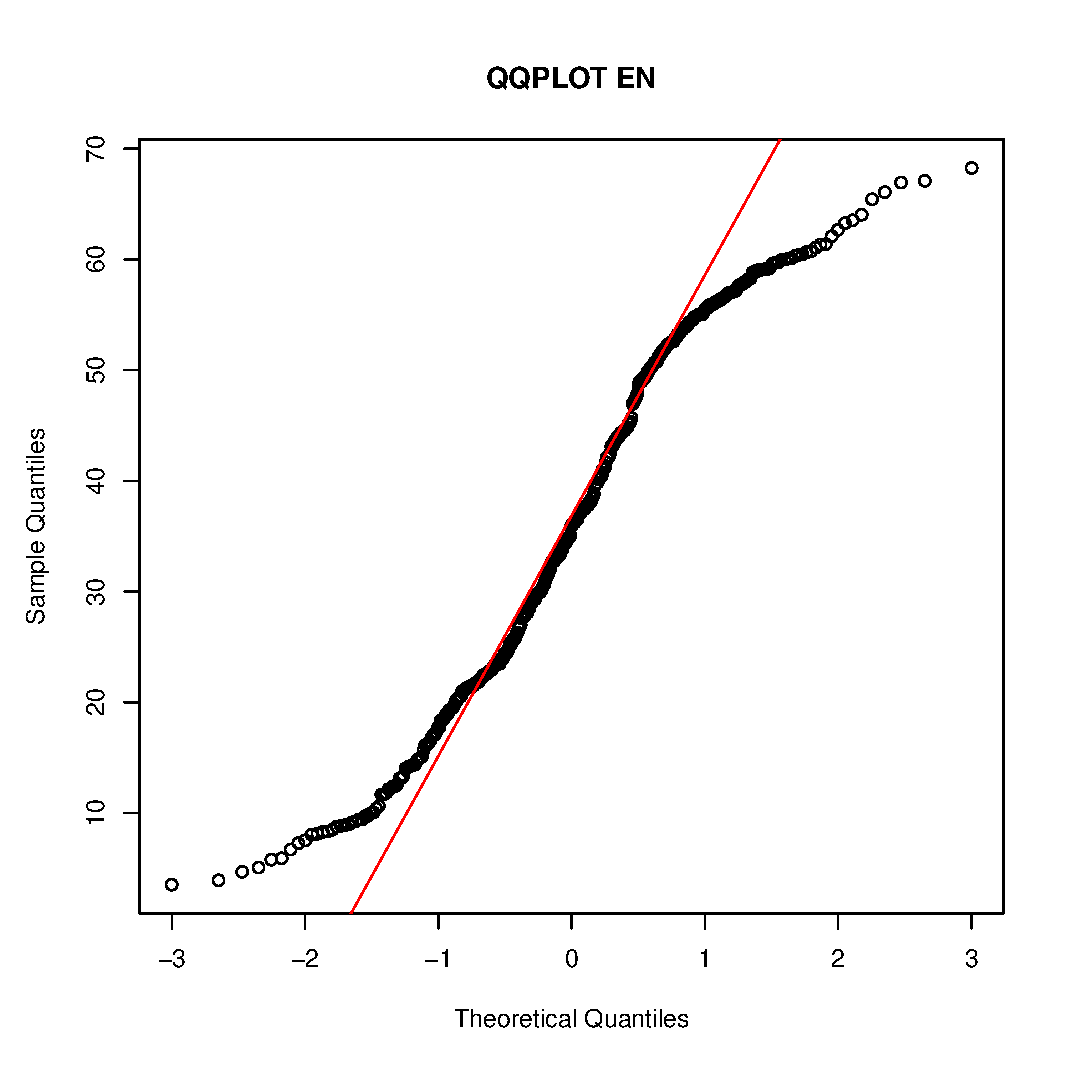
\includegraphics[height=5cm,width=6cm]{figures/EN_QQ.eps}
%DIFDELCMD < 	%%%
%DIFDELCMD < \caption{%
{%DIFAUXCMD
\DIFdel{QQ-plot of EN monthly capacity factor time series ranging from January 1981 to December 2011.}}
	%DIFAUXCMD
%DIFDELCMD < \label{qq_EN}
%DIFDELCMD < \end{figure}
%DIFDELCMD < %%%
\DIFdelend %DIF > \item Apply the conditional sampling technique (see \cite{cherubini2004copula}), in order to generate conditioned values of PIT variables, i.e., $\{\mathbf{u}_{t}^{*(1) }\}_{t=t+1}^{t+k}$;

\DIFdelbegin %DIFDELCMD < \begin{figure}[htbp]
%DIFDELCMD < 	\centering
%DIFDELCMD < 	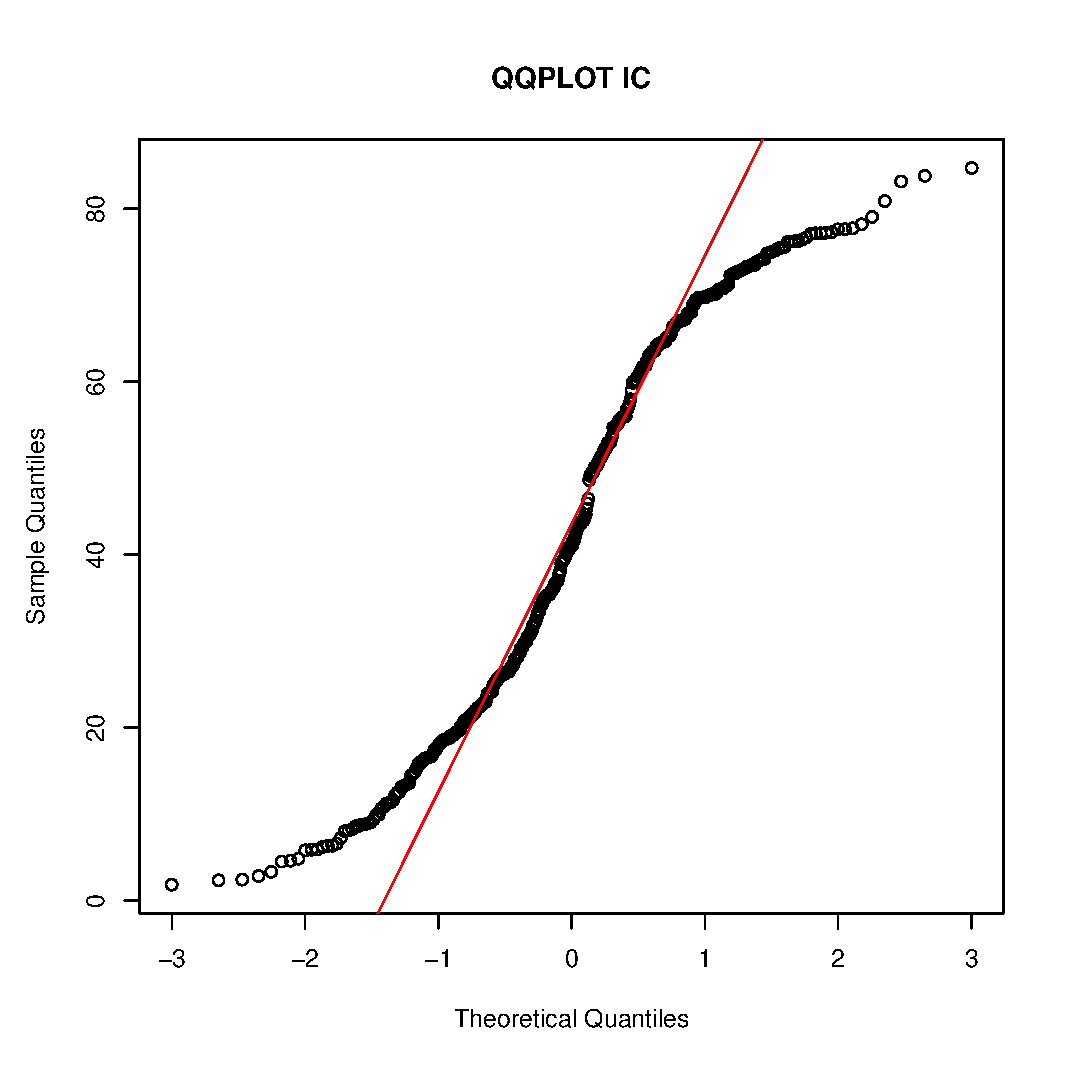
\includegraphics[height=5cm,width=6cm]{figures/IC_QQ.eps}
%DIFDELCMD < 	%%%
%DIFDELCMD < \caption{%
{%DIFAUXCMD
\DIFdel{QQ-plot of IC monthly capacity factor time series ranging from January 1981 to December 2011.}}
	%DIFAUXCMD
%DIFDELCMD < \label{qq_IC}
%DIFDELCMD < \end{figure}
%DIFDELCMD < %%%
\DIFdelend %DIF > \item Since it is a fully parametric copula model, marginal densities are assumed to be are known. Calculate the quantile of a beta density function evaluated at $\{\mathbf{u}_{t}^{*(1)}\}_{t=t+1}^{t+h}$, where the first shape parameter $\beta_{i,t}=exp\{f_{i,t}\}$ was already calculated to generate the forecasting set $S_k \, \forall \, k \in K$ and the second one $\alpha\in\hat{\theta}$. %In a nutshell, $y^{*(m)}_{k,t+h}=F_{beta}^{-1}(u_{t+h}^{*(m)}| f_{k,t},\mathcal{F}_{k,t-1},\hat{\theta}_{k})$.

\DIFdelbegin %DIFDELCMD < \begin{figure}[htbp]
%DIFDELCMD < 	\centering
%DIFDELCMD < 	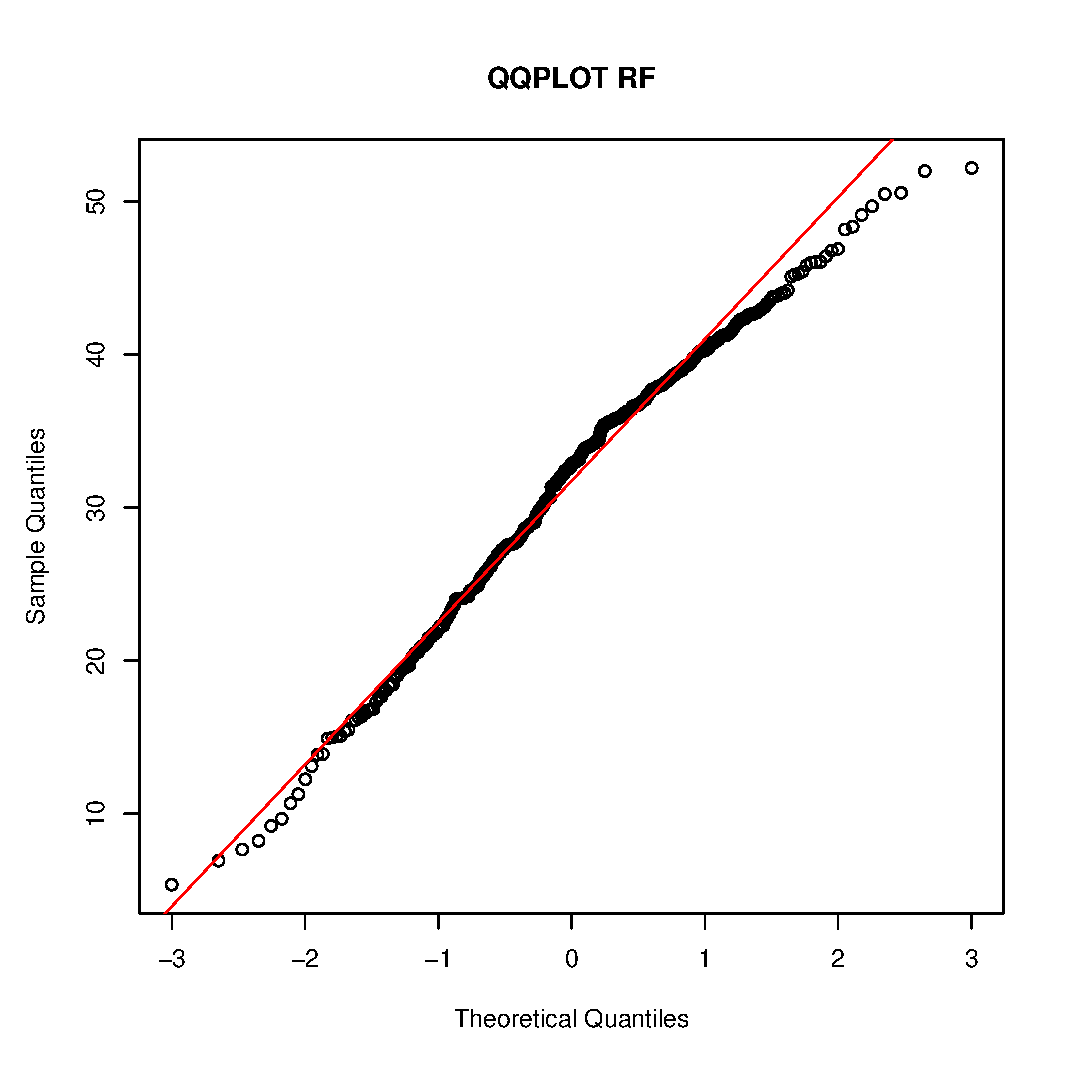
\includegraphics[height=5cm,width=6cm]{figures/RF_QQ.eps}
%DIFDELCMD < 	%%%
%DIFDELCMD < \caption{%
{%DIFAUXCMD
\DIFdel{QQ-plot of RF monthly capacity factor time series ranging from January 1981 to December 2011.}}
	%DIFAUXCMD
%DIFDELCMD < \label{qq_RF}
%DIFDELCMD < \end{figure}
%DIFDELCMD < %%%
\DIFdelend %DIF > \item Repeat the above steps until $m=2000$.
%DIF > \end{enumerate}
\DIFaddbegin 



%DIF > %%%%%%%%%%%%%%%%%%%%%%%%%%%%%%%%%%%%%%%%%%%%%%%%%%%%%%%%%%%%%%%%%%%%%%%%%%%%%%%%%%%%%%%%%%%%%%%%%%%%%%%%%%%%%%%%%%%%%%%
%DIF >  ===== Sec. IV - Case Study ===== %

\section{\DIFadd{Case Study - Simulating medium and long-term joint scenarios}} \label{Application}
\DIFaddend 

Our time series data comprises monthly \DIFdelbegin \DIFdel{wind CF}\DIFdelend \DIFaddbegin \DIFadd{WPG}\DIFaddend , from January 1981 to December 2011, measured at three wind plants located in the Brazilian Northeast, namely: Rio do Fogo (RF), Icaraizinho (IC) and Enacel (EN). The last year of these time series were kept for out of sample \DIFdelbegin \DIFdel{forecasting evaluation. }\DIFdelend \DIFaddbegin \DIFadd{scenario evaluation. The intrinsic non-Gaussian nature of WPG time series can be easily shown by observing the shape of a qq-plot or by running a simple normality test, such as the Jarque-Bera test. Considering individually each of the three time series of WPG, the null hypothesis of normality for each of these time series has been rejected (p-values $<$ 0.001). Likewise, considering QQ-plot depicted in Figure \ref{qq_IC} of IC unit, it strongly suggest non normality through the observed positive skewness, which suggest strong adequacy of our proposed beta GAS model.
}

%DIF > \begin{figure}[htbp]
%DIF > 	\centering
%DIF > 	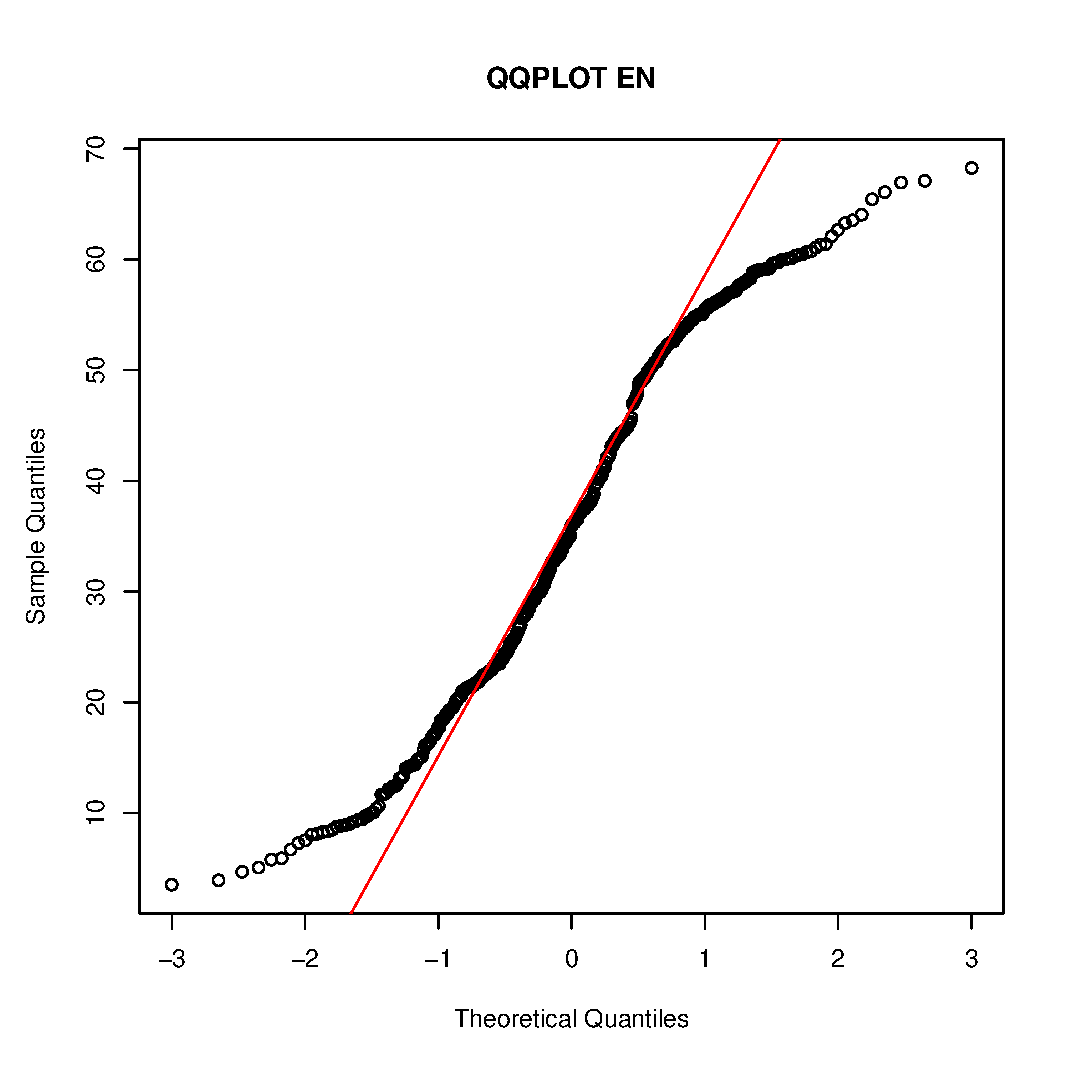
\includegraphics[height=5cm,width=6cm]{figures/EN_QQ.eps}
%DIF > 	\caption{QQ-plot of EN monthly capacity factor time series ranging from January 1981 to December 2011.}
%DIF > 	\label{qq_EN}
%DIF > \end{figure}

\begin{figure}[htbp]
	\centering
	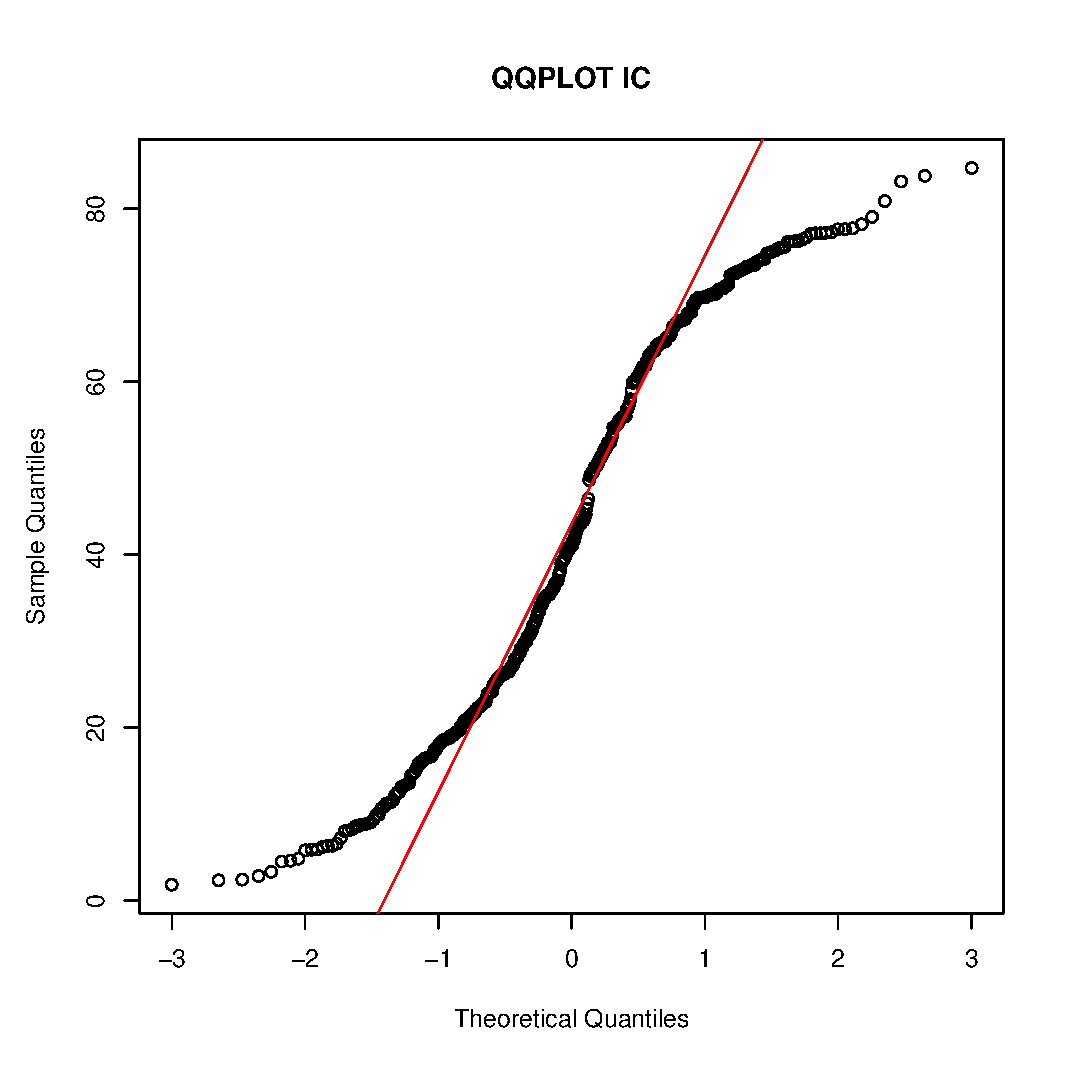
\includegraphics[height=5cm,width=6cm]{figures/IC_QQ.eps}
	\caption{\DIFaddFL{QQ-plot of IC monthly capacity factor time series ranging from January 1981 to December 2011.}}
	\label{qq_IC}
\end{figure}

%DIF > \begin{figure}[htbp]
	%DIF > \centering
	%DIF > 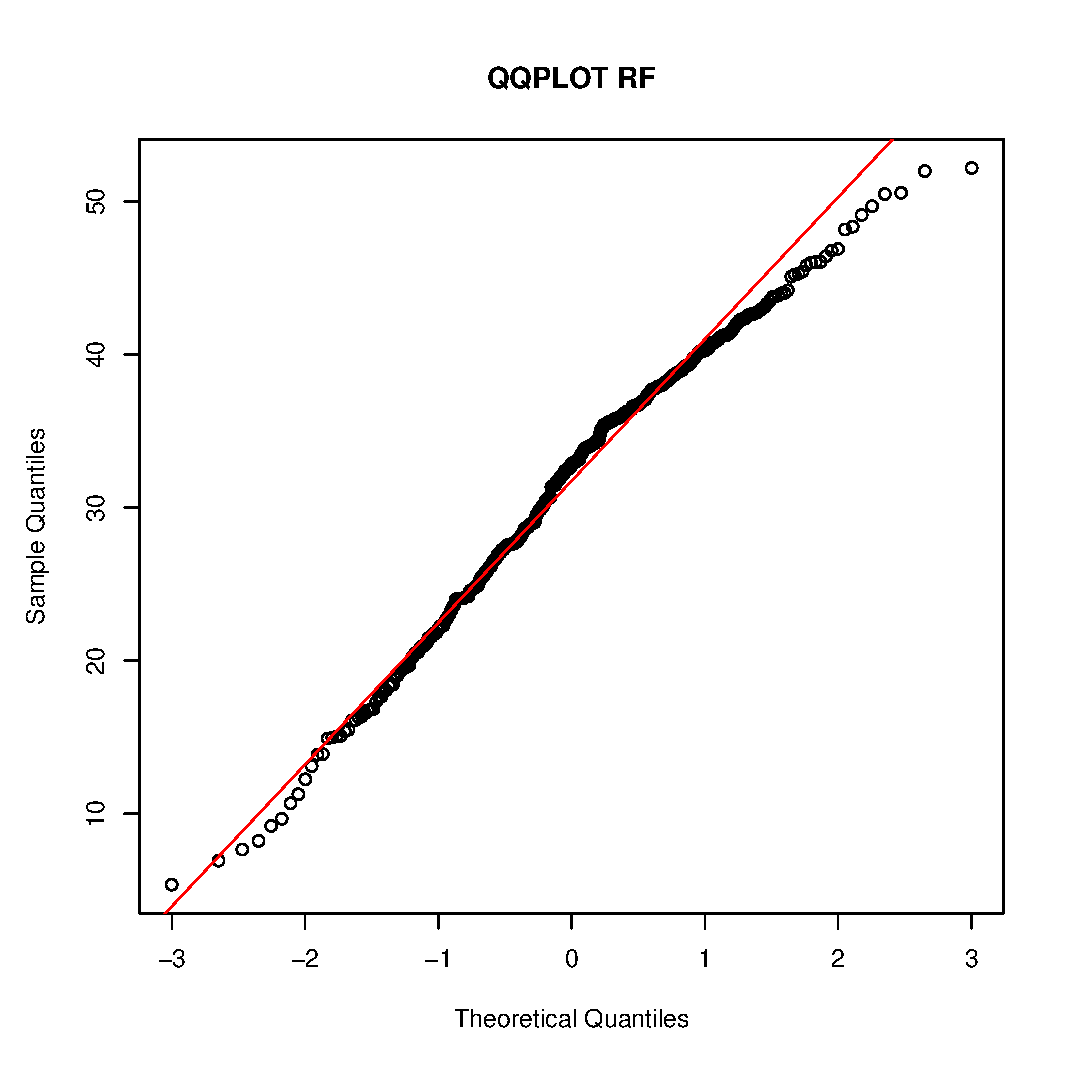
\includegraphics[height=5cm,width=6cm]{figures/RF_QQ.eps}
	%DIF > \caption{QQ-plot of RF monthly capacity factor time series ranging from January 1981 to December 2011.}
	%DIF > \label{qq_RF}
%DIF > \end{figure}
\DIFaddend 

\DIFdelbegin \DIFdel{Firstly, parameters of the beta GAS(p, q) models are estimated via maximum likelihood. To accommodate outliers, dummy variables ($d_{t}$) were used where appropriate (for details see Table \ref{table1}). }\DIFdelend In this study, the same lag structure was used for the three \DIFdelbegin \DIFdel{wind plants }\DIFdelend \DIFaddbegin \DIFadd{WPG }\DIFaddend time series, as presented in Equation \eqref{eq:2}. After removing the first and last years of data for initial values estimation and \DIFdelbegin \DIFdel{forecasting evaluation }\DIFdelend \DIFaddbegin \DIFadd{scenario evaluation respectively}\DIFaddend , maximization of the \DIFdelbegin \DIFdel{likelihood }\DIFdelend \DIFaddbegin \DIFadd{log-likelihood }\DIFaddend function resulted in the estimated parameters presented in Table \ref{table1}. \DIFaddbegin \DIFadd{Dummy variables $D_t$ were introduced until quantile residuals show no more auto correlation structure. The way to choose in which time index $t$ a dummy variable $D_t$ should be introduced is by checking, after model fit, where $|r_{t,\hat{\theta}_i}|>3$, since under the Gaussianity of the residuals, 3 times the standard deviation reflects an abnormal value. 
}\DIFaddend 

\begin{table}[htbp]
\centering
\caption{Maximum likelihood estimation of the beta GAS \DIFdelbeginFL \DIFdelFL{(12,12) }\DIFdelendFL model applied to three Brazilian wind plants.}
\DIFdelbeginFL %DIFDELCMD < \label{my-label}
%DIFDELCMD < %%%
\DIFdelendFL \begin{tabular}{ccccccc}
\multirow{2}{*}{Parameter} & \multicolumn{2}{c}{Rio do Fogo (RF)} & \multicolumn{2}{c}{Icaraizinho (IC)} & \multicolumn{2}{c}{Enacel (EN)} \\
                           & Estim.     & S.E.      & Estim.     & S.E.      & Estim.     & S.E.      \\ \hline
$A_{1}$                    & 0.551      & 0.006     & 0.539     & 0.071      & 0.540      & 0.060     \\
$A_{2}$                    & 0.231      & 0.004     & -0.226      & 0.066     & 0.498     & 0.073     \\
$A_{3}$                    & -0.147     & 0.007     & 0.352      & 0.070     & 0.041      & 0.053     \\
$A_{11}$                   & 0.008      & 0.007     & 0.219      & 0.038     & 0.169      & 0.034     \\
$A_{12}$                   & 0.110       & 0.004     & -0.176      & 0.043     & 0.228     & 0.031     \\
$B_{1}$                    & -0.080      & 0.002     & 1.058      & 0.055     & -0.164      & 0.039     \\
$B_{2}$                    & 0.441      & 0.006     & -0.818     & 0.043     & -0.186     & 0.036     \\
$B_{3}$                    & -0.369     & 0.011     & 0.156    & 0.031     & -0.008       & 0.016     \\
$B_{11}$                   & 0.207      & 0.013     & 0.227      & 0.016     & -0.004       & 0.005      \\
$B_{12}$                   & 0.325      & 0.011     & 0.121      & 0.037     & 0.721      & 0.035     \\
$\omega$                   & 3.139      & 0.019     & 2.571     & 0.260     & 5.485      & 0.780     \\
$\alpha$                   & 9.408      & 0.042     & 10.244     & 0.791     & 9.293      & 0.515     \\
\DIFdelbeginFL \DIFdelFL{$d_{t=21}^{(Set, 1983)}$   }\DIFdelendFL \DIFaddbeginFL \DIFaddFL{$D_{t=21}^{(Set, 1983)}$   }\DIFaddendFL & -          & -         & 2.320      & 0.287     & 1.447          & 0.247         \\
\DIFdelbeginFL \DIFdelFL{$d_{t=22}^{(Oct, 1983)}$   }\DIFdelendFL \DIFaddbeginFL \DIFaddFL{$D_{t=22}^{(Oct, 1983)}$   }\DIFaddendFL & -          & -         & 2.021      & 0.309     & 3.610      & 0.481     \\
\DIFdelbeginFL \DIFdelFL{$d_{t=29}^{(May, 1984)}$   }\DIFdelendFL \DIFaddbeginFL \DIFaddFL{$D_{t=29}^{(May, 1984)}$   }\DIFaddendFL & -          & -         & -0.031      & 0.641     & -          & -     \\
\DIFdelbeginFL \DIFdelFL{$d_{t=129}^{(Sep, 1992)}$  }\DIFdelendFL \DIFaddbeginFL \DIFaddFL{$D_{t=129}^{(Sep, 1992)}$  }\DIFaddendFL & -          & -         & 3.349      & 0.317     & 1.675      & 0.386     \\
\DIFdelbeginFL \DIFdelFL{$d_{t=130}^{(Oct, 1992)}$  }\DIFdelendFL \DIFaddbeginFL \DIFaddFL{$D_{t=130}^{(Oct, 1992)}$  }\DIFaddendFL & -          & -         & -          & -         & 1.189      & 0.345     \\
\DIFdelbeginFL \DIFdelFL{$d_{t=165}^{(Sep, 1995)}$  }\DIFdelendFL \DIFaddbeginFL \DIFaddFL{$D_{t=165}^{(Sep, 1995)}$  }\DIFaddendFL & -          & -         & 1.460      & 0.264     & -          & -     \\
\DIFdelbeginFL \DIFdelFL{$d_{t=241}^{(Jan, 2002)}$  }\DIFdelendFL \DIFaddbeginFL \DIFaddFL{$D_{t=241}^{(Jan, 2002)}$  }\DIFaddendFL & -          & -         & -          & -         &-1.527      & 0.582     \\
\DIFdelbeginFL \DIFdelFL{$d_{t=308}^{(Aug, 2007)}$  }\DIFdelendFL \DIFaddbeginFL \DIFaddFL{$D_{t=308}^{(Aug, 2007)}$  }\DIFaddendFL & 1.771      & 0.346     & -          & -         & -          & -         \\
\DIFdelbeginFL \DIFdelFL{$d_{t=309}^{(Sep, 2007)}$  }\DIFdelendFL \DIFaddbeginFL \DIFaddFL{$D_{t=309}^{(Sep, 2007)}$  }\DIFaddendFL & 2.384      & 0.369     & -          & -         & -          & -         \\
\DIFdelbeginFL \DIFdelFL{$d_{t=345}^{(Sep, 2010)}$  }\DIFdelendFL \DIFaddbeginFL \DIFaddFL{$D_{t=345}^{(Sep, 2010)}$  }\DIFaddendFL & 3.004      & 0.277     & -          & -         & -          & -         \\
\DIFdelbeginFL \DIFdelFL{$d_{t=346}^{(Oct, 2010)}$  }\DIFdelendFL \DIFaddbeginFL \DIFaddFL{$D_{t=346}^{(Oct, 2010)}$  }\DIFaddendFL & -          & -         & -1.462     & 0.350     & -          & - \\\hline
\end{tabular}
\label{table1}
\end{table}

Finally, to investigate correct model specification\DIFdelbegin \DIFdel{Table \ref{table2} report the results for the }\DIFdelend \DIFaddbegin \DIFadd{, a fully detailed analysis in the quantile residuals was undertaken and reported in Table \ref{table2}. }\DIFaddend Jarque-Bera test for normality (under the correct specification of the beta density, the residuals should be normally distributed), Ljung-Box test for absence of autocorrelation and Ljung-Box on the squared residuals to check for ARCH \DIFdelbegin \DIFdel{effect }\DIFdelend \DIFaddbegin \DIFadd{effects were considered }\DIFaddend (both were conducted using \DIFaddbegin \DIFadd{until lag }\DIFaddend 30\DIFdelbegin \DIFdel{lags). %DIF < To evaluate the model diagnostics, a fully detailed analysis in the time series quantile residuals was attended. The previously described diagnostic tests were applied, Jarque Bera test for normality, Ljung-Box and ARCH effects for autocorrelation. All the tests were conducted until lag 30 and their results are shown in Table \ref{table2}.
}\DIFdelend \DIFaddbegin \DIFadd{). As reported in Table \ref{table2}, there were no rejections of the null hypothesis in none of the tests, hence it can be concluded that the proposed beta GAS models are adequate to describe the three time series of WPG.
}\DIFaddend 

\begin{table}[htbp]
%\begin{table}[]
\centering
\caption{P-values of standard diagnostic tests.}
\begin{tabular}{c|ccc}
\hline
{\bf Test}      & {\bf Rio do Fogo} & {\bf Icaraizinho} & {\bf Enacel} \\ \hline
Normality       & 0.242             & 0.582            & 0.386         \\
Autocorrelation & 0.174             & 0.854            & 0.127         \\
Arch effect     & 0.703             & 0.479            & 0.175         \\ \hline
\end{tabular}
\label{table2}
\end{table}

\DIFdelbegin \DIFdel{From Table \ref{table2}, it can be concluded that the proposed beta GAS (12,12) models are adequate to describe the three time series of CF's. For forecasting evaluation the prediction of the GAS models were compared to those obtained from the fitting of a SARIMA model to the logarithm of the CF time series. To obtain the prediction for the original CF's series these values have to be exponentiated. As it is known, exponentiation of Gaussian values can result in unrealistically large values for the original variable. This will not be the case with GAS models since from the outset the chosen probability model is appropriate to the support of the response variable. To provide some evidence on the distortion brought by the anti log transformation, as an evidence, we fitted a Gaussian SARIMA model to the log of the three CF time series wind plants consired here (EN,IC,RF) , and simulated 2000 scenarios 12 steps ahead. Then we compared the empirical quantiles obtained from the simulated CF series to }\DIFdelend %DIF > {\color{red} After model fit, one should follow steps \ref{step1_uni}-\ref{step3_uni} of Part I in \ref{univariate_modelling} to generate future scenarios of WPG time series for each one of the $K$ units. We produced 2000, $m=1,...,2000$, scenarios for each of the $h$ steps ahead forecasting horizon $h=1,2,...,12$. The median, at each step $h$, of those scenarios are compared to those obtained from fitting a SARIMA model to the logarithm of the WPG time series, adopting the same dummy variables $D_t$ which were used to fit the beta GAS models. Nevertheless, when using the SARIMA model, to obtain the prediction for the original WPG time series, these values have to be exponentiated. As it is known, exponentiation of Gaussian values can result in unrealistically large values for the original variable. This will not be the case with GAS models since from the outset the chosen probability model is appropriate to the support of the response variable. Goodness of fit results as shown in Table \ref{tablefor} indicates that our model seems competitive when compared to the benchmark SARIMA model.}
\DIFaddbegin 

\DIFadd{Although the forecasts of our beta GAS model are superior to }\DIFaddend the \DIFdelbegin \DIFdel{quantiles of the original CF series(both in the original scale) $Q^{(\alpha\%)}\, \forall \,\alpha \in \{0.05, 0.10, 0.5, 0.9, 0.95 \}$ which are depicted in Figure \ref{analise_cenarios_SARIMA}.As a result, the simulated quantiles are far beyond the historical quantiles of the CF time series, indicating the distortions brought by fitting the model to }\DIFdelend \DIFaddbegin \DIFadd{ones obtained using a simple SARIMA model, we advocate that the main contribution of the proposed framework here is not to improve the conditional mean forecast. Alternatively, }\DIFaddend the \DIFdelbegin \DIFdel{log of the series.
	}%DIFDELCMD < 

%DIFDELCMD < %%%
%DIF < \begin{figure}[htbp]
%DIF < \centering
%DIF < \includegraphics[height=6cm,width=9.0cm]{figures/IC_COM_LOG.pdf}
%DIF < \caption{2000 simulations of 12 steps ahead using SARIMA model in the %log of time series of Icaraizinho CF.}
%DIF < \label{SARIMA_COM_TRANS}
%DIF < \end{figure}
%DIFDELCMD < 

%DIFDELCMD < %%%
%DIF < \begin{figure}[htbp]
%DIF < \centering
%DIF < \includegraphics[height=5.3cm,width=8.0cm]{IC_COM_LOG.ps}
%DIF < \caption{2000 simulations of 12 steps ahead using SARIMA model in the %log of time series of Icaraizinho CF.}
%DIF < \label{SARIMA_COM_TRANS}
%DIF < \end{figure}
%DIFDELCMD < 

%DIFDELCMD < %%%
%DIF < \begin{figure}[htbp]
%DIF < \centering
%DIF < 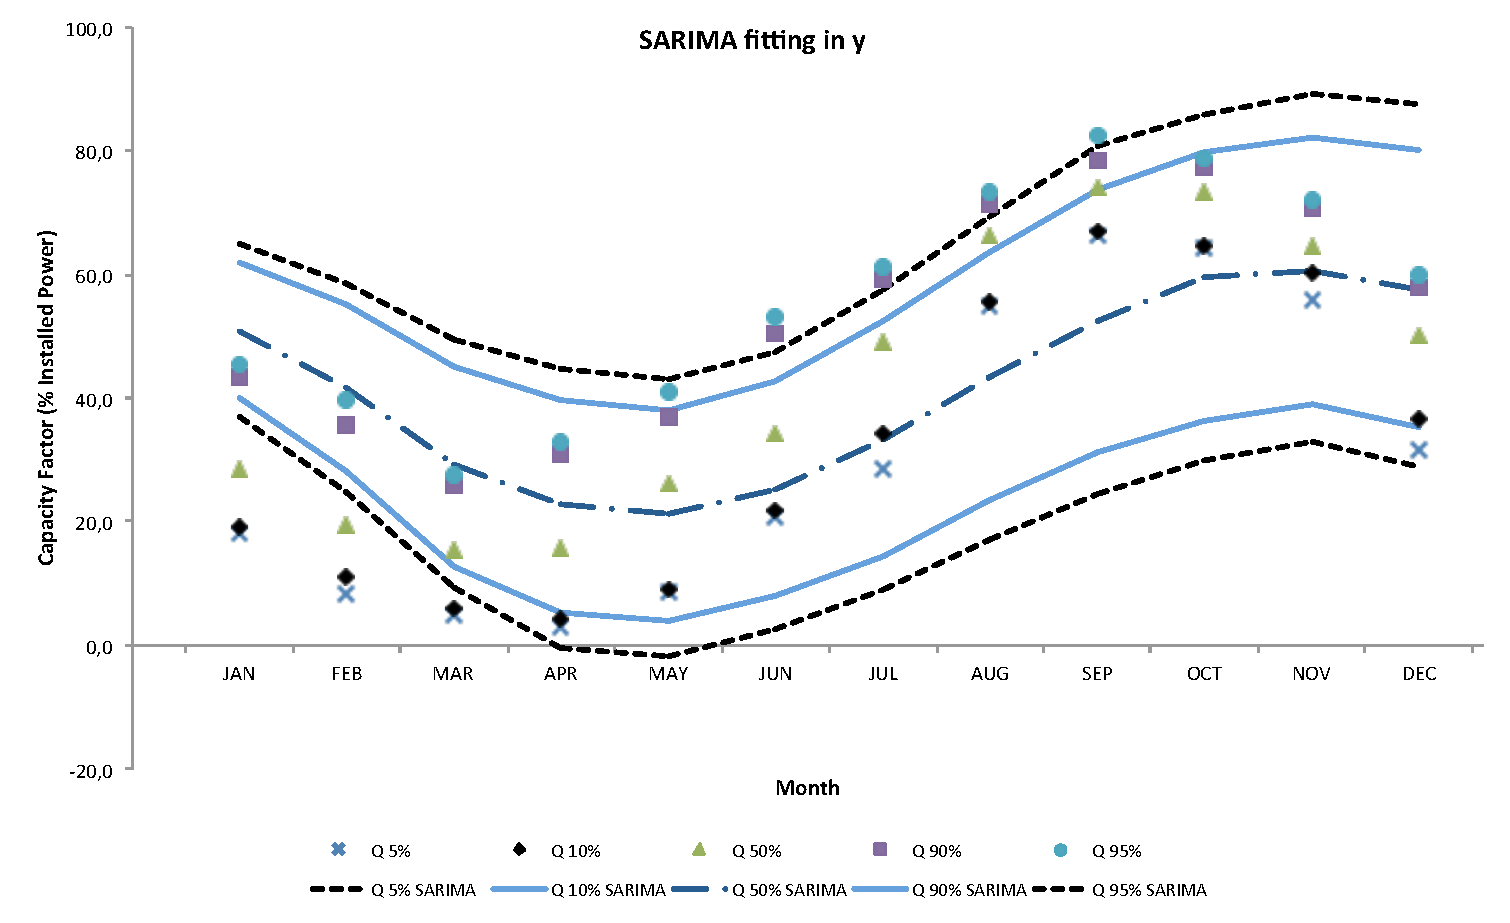
\includegraphics[height=5.3cm,width=8.0cm]{figures/SARIMA_SEM_LOG.pdf}
%DIF < \caption{Monte carlo simulation (2000) of 12 steps ahead using SARIMA %model with log transformation of Icaraizinho CF time series.}
%DIF < \label{SARIMA_COM_LOG}
%DIF < \end{figure}
%DIFDELCMD < 

%DIFDELCMD < %%%
%DIF < The VAR model used here is similar to the VARX model from \cite{FosteringWPP}, nonetheless without exogenous variables. 
\DIFdel{The $k$ steps ahead distribution conditional on observations up to time $t$}\DIFdelend \DIFaddbegin \DIFadd{main goal of the proposed methodology is 1) to enhance the whole PDF description for individual time series, e.g.}\DIFaddend , \DIFdelbegin \DIFdel{$p(y_{t+k}|\mathcal{F}_{t} )$, used to obtain out of sample forecasts, has no analytical form in GAS models, and therefore is estimated using Monte Carlo simulation. We produced 2000 scenarios for each of the $k$ ahead forecasting horizon $k=1,2,...,12$. Goodness of fit results as shown in Table \ref{tablefor} indicates that our model seems competitive when compared to the benchmark SARIMA model}\DIFdelend \DIFaddbegin \DIFadd{extreme quantiles are better approximated under the proposed framework, and 2) to enhance the multivariate description by capturing the spatial dependence among time series (generally located at different geographical areas) through a time-varying copula}\DIFaddend .

\begin{table}[htbp]
\centering
\caption{Forecasting evaluation between beta GAS(12,12) and SARIMA model.}
\begin{tabular}{c|cccc}
\hline
Modelo                 & Medidas        & RF    & IC     & EN     \\ \hline
                       & RMSE           & 5.639 & 6.181  & 8.736  \\
beta GAS(12,12)        & MAE            & 5.209 & 5.021  & 7.346  \\
                       & Pseudo R$^{2}$ & 0.834 & 0.941  & 0.875  \\ \hline
                       & RMSE           & 7.566 & 10.668 & 9.737  \\
SARIMA                 & MAE            & 6.263 & 7.675  & 8.222  \\
                       & Pseudo R$^{2}$ & 0.809 & 0.831  & 0.859  \\ \hline
\end{tabular}
\label{tablefor}
\end{table}

\DIFdelbegin \DIFdel{The main contribution of the proposed framework here is not to improve the conditional mean forecast. The methodology is devote to improve the modelling of the join density of wind CF, providing accurate scenarios that take into account the dependency structure among different geographical areas.
}%DIFDELCMD < 

%DIFDELCMD < %%%
\DIFdelend In the following we will \DIFdelbegin \DIFdel{provide details on }\DIFdelend \DIFaddbegin \DIFadd{conduct }\DIFaddend the multivariate modeling of the three \DIFdelbegin \DIFdel{CF }\DIFdelend \DIFaddbegin \DIFadd{WPG }\DIFaddend time series using the \DIFdelbegin \DIFdel{dynamic copula approach }\DIFdelend \DIFaddbegin \DIFadd{second step GAS procedure }\DIFaddend previously described in \DIFdelbegin \DIFdel{Section \ref{copula}. After estimating the fixed parameter vector $\hat{\theta}_{i}$ of each marginal $i \in I$, PIT variables $u_{it}$ are generated using the whole set of information up to time $t$, $\mathcal{F}_{t}$. Then, in order to estimate the copula parameters , the multi-stage optimization approach, IFM is used. The }\DIFdelend \DIFaddbegin \DIFadd{\ref{step1_multi}-\ref{step4_multi} of Part II in \ref{multivariate_modelling}. The copula parameters were estimated and its values are displayed in Table \ref{tab_3}. Regarding its }\DIFaddend degrees of freedom\DIFdelbegin \DIFdel{of the copula model }\DIFdelend \DIFaddbegin \DIFadd{, it }\DIFaddend was estimated using \DIFdelbegin \DIFdel{the }\DIFdelend profile likelihood process \DIFdelbegin \DIFdel{(see \mbox{%DIFAUXCMD
\cite{murphy2000profile}
}%DIFAUXCMD
), resulting }\DIFdelend \DIFaddbegin \DIFadd{which resulted }\DIFaddend in $\hat{\nu}=340$\DIFdelbegin \DIFdel{is the value that maximizes the log likelihood, which means }\DIFdelend \DIFaddbegin \DIFadd{. Such value of degrees of freedom points out }\DIFaddend that the proposed elliptical copula reduces itself to a time-varying Gaussian copula\DIFdelbegin \DIFdel{. %DIF < This process made our approach feasible, since it is easier to evaluate the log likelihood function without maximizing simultaneously $\nu$ and $\theta^{Cop}$.
}%DIFDELCMD < 

%DIFDELCMD < %%%
\DIFdel{The model procedure involving the elliptical copula presented in Section \ref{copula} was applied to the $T \times I$ vector $\tilde{y}_{t}^{'}=[F_{\nu}^{-1}(u_{1t}), F_{\nu}^{-1}(u_{2t}), F_{\nu}^{-1}(u_{3t})]^{'}$. From now on, this will be referred as t-GAS(p, q). In our application, the updating mechanism of the copula parameter with $p=1$ and $q=1$ was shown satisfactory. Table \ref{tab_3}. presents the results for the estimation of the parameters for the t-GAS(1}\DIFdelend , \DIFdelbegin \DIFdel{1) model.
   %DIF < The results of static parameter vector of the t-GAS(1,1) are presented in Table \ref{tab_3}.
}\DIFdelend \DIFaddbegin \DIFadd{which makes perfect sense since we are dealing with monthly data.
   }\DIFaddend 

\begin{table}[htbp]
\centering
\caption{Maximum likelihood estimation of the \DIFdelbeginFL \DIFdelFL{t-GAS(1,1) }\DIFdelendFL \DIFaddbeginFL \DIFaddFL{second step GAS }\DIFaddendFL model applied to \DIFaddbeginFL \DIFaddFL{the PIT variables of }\DIFaddendFL three Brazilian wind plants.}
\label{my-label2}
\begin{tabular}{c|cc}
\hline
\multirow{2}{*}{{\bf Parameter}} & \multicolumn{2}{c}{{\bf t-GAS}}                       \\
                                 & \multicolumn{1}{l}{Estim.} & \multicolumn{1}{l}{S.E.} \\\hline
\DIFdelbeginFL \DIFdelFL{$\omega$                               }\DIFdelendFL \DIFaddbeginFL \DIFaddFL{$\Omega$                         }\DIFaddendFL & 1.589                      & 0.063                    \\
\DIFdelbeginFL \DIFdelFL{A                                }\DIFdelendFL \DIFaddbeginFL \DIFaddFL{$\Pi$                            }\DIFaddendFL & 0.354                      & 0.017                    \\
\DIFdelbeginFL \DIFdelFL{B                                }\DIFdelendFL \DIFaddbeginFL \DIFaddFL{$\Upsilon$                       }\DIFaddendFL & 0.425                      & 0.083                    \\\hline
\end{tabular}
\label{tab_3}.
\end{table}

From Table \ref{tab_3}, it follows that all parameters are statistically significant at 5\%\DIFdelbegin \DIFdel{or less which implies that the correlation of the elliptical copula is indeed time-varying}\DIFdelend \DIFaddbegin \DIFadd{, or less}\DIFaddend . The value of the parameter \DIFdelbegin \DIFdel{$A$, in the copula model, reinforce }\DIFdelend \DIFaddbegin \DIFadd{$\Pi$ plays a key role here, since it reinforces }\DIFaddend the fact that \DIFdelbegin \DIFdel{the association between these three wind plants }\DIFdelend \DIFaddbegin \DIFadd{dependence structure among these three WPG time series }\DIFaddend might not be static over the analyzed period. \DIFdelbegin \DIFdel{It is important to mention that such feature will be contemplated when simulating values from the joint density through our proposed methodology.%DIF < Figures \ref{elementos_Sigma_RFxIC}, \ref{elementos_Sigma_RFxEN} and \ref{elementos_Sigma_ICxEN} depict the plot of this correlations in time. Such Figures reinforce the fact that the association between these three wind plants might not be static over the analyzed period. It is important to mention that such feature will be contemplated when simulating values from the joint density through our proposed methodology.
   }%DIFDELCMD < 

%DIFDELCMD < %%%
%DIF < \begin{figure}[htbp]
%DIF < \centering
%DIF < 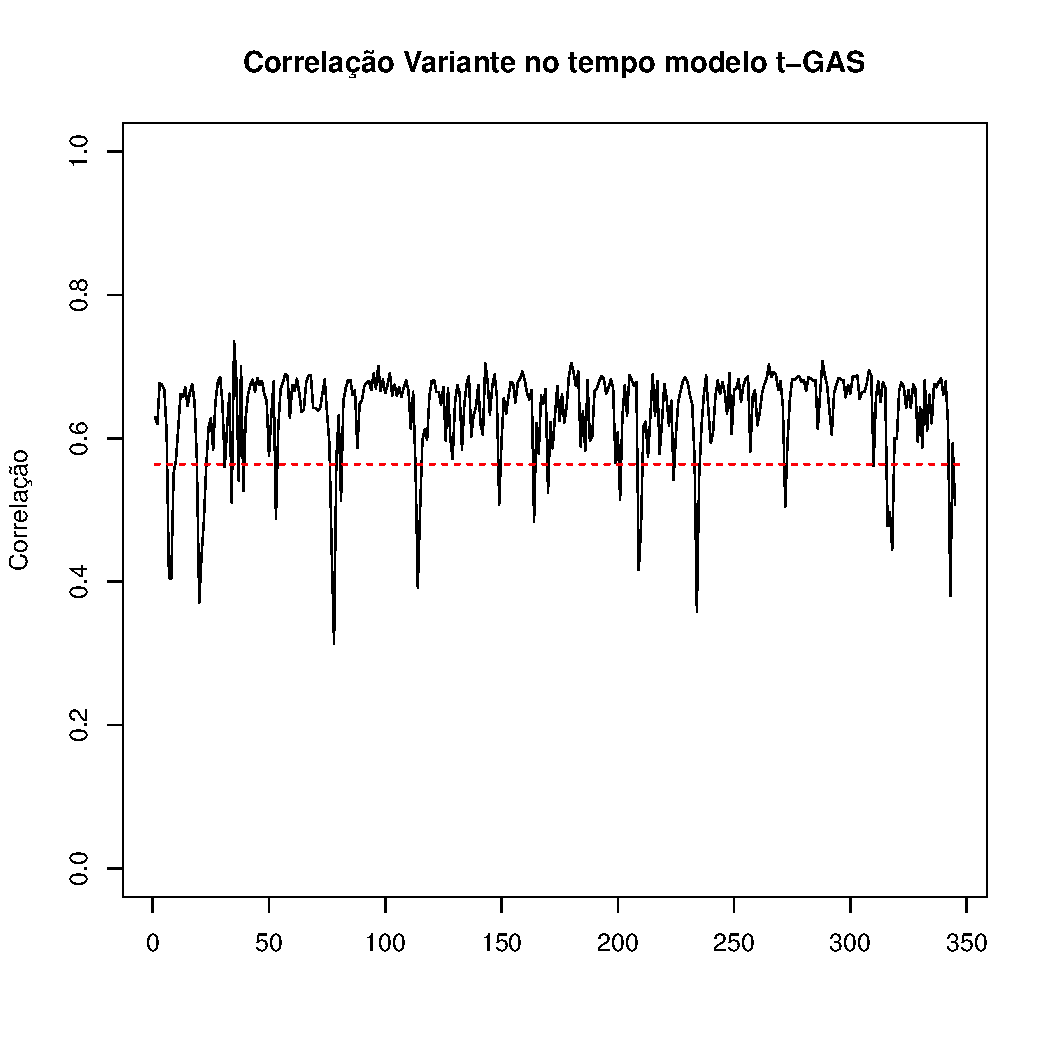
\includegraphics[height=6.9cm,width=6.9cm]{figures/roh_VT_RFxIC.pdf}
%DIF < \caption{Elementos de $\hat{\Sigma_{t}}$ atualizados pelo mecanismo GAS entre $\tilde{y}_{1t}$ e $\tilde{y}_{2t}$, que representam as usinas de RF e IC respectivamente.}
%DIF < \label{elementos_Sigma_RFxIC}
%DIF < \end{figure}
%DIF < 
%DIF < \begin{figure}[htbp]
%DIF < \centering
%DIF < 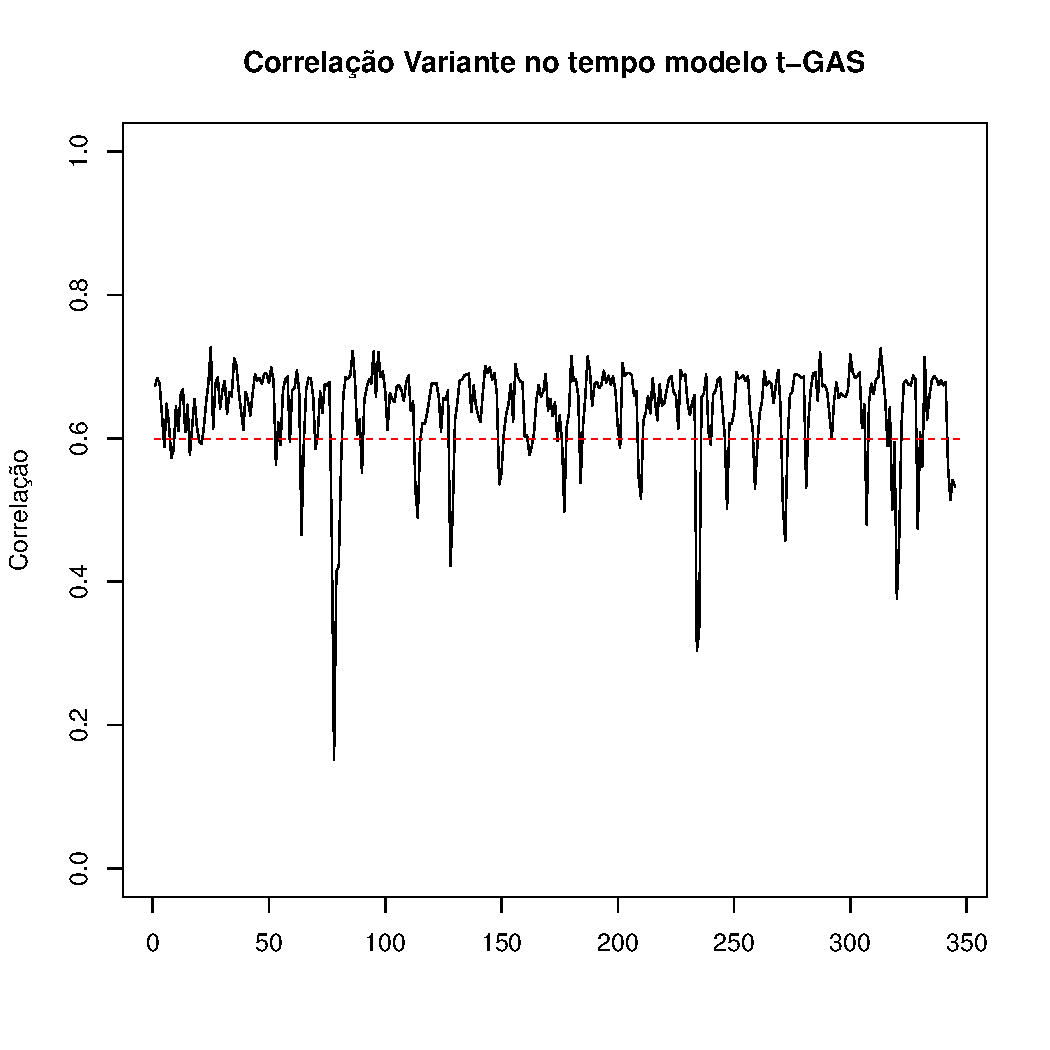
\includegraphics[height=6.9cm,width=6.9cm]{figures/roh_VT_RFxEN.pdf}
%DIF < %\includegraphics[height=6.9cm,width=6.9cm]{figures/roh_VT_RFxEN_gauss.eps}
%DIF < \caption{Elementos de $\hat{\Sigma_{t}}$ atualizados pelo mecanismo GAS entre $\tilde{y}_{1t}$ e $\tilde{y}_{3t}$, que representam as usinas de RF e EN respectivamente.}
%DIF < \label{elementos_Sigma_RFxEN}
%DIF < \end{figure}
%DIF < 
%DIF < \begin{figure}[htbp]
%DIF < \centering
%DIF < 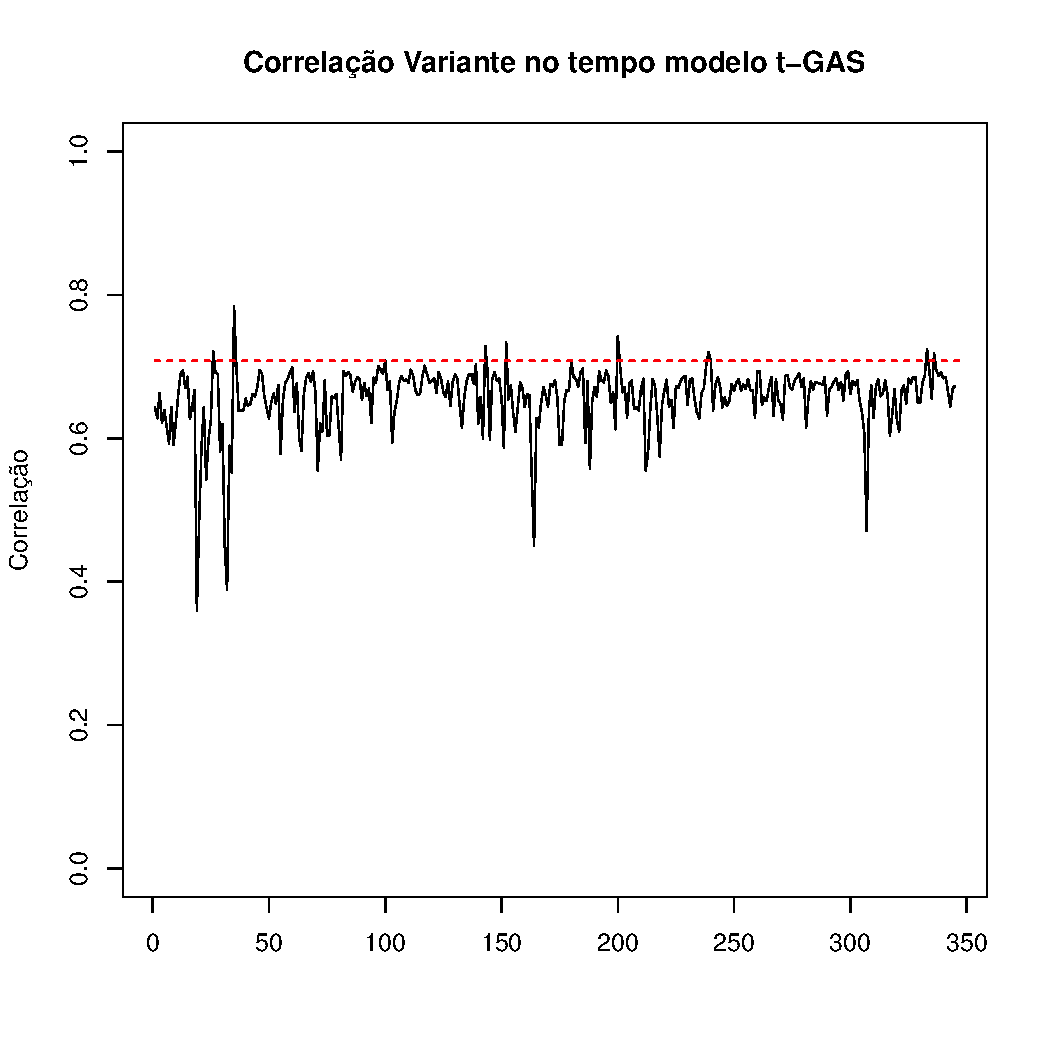
\includegraphics[height=6.9cm,width=6.9cm]{figures/roh_VT_ICxEN.pdf}
%DIF < %\includegraphics[height=6.9cm,width=6.9cm]{figures/roh_VT_ICxEN_gauss.eps}
%DIF < \caption{Elementos de $\hat{\Sigma_{t}}$ atualizados pelo mecanismo GAS entre entre $\tilde{y}_{2t}$ e $\tilde{y}_{3t}$, que representam as usinas de IC e EN respectivamente.}
%DIF < \label{elementos_Sigma_ICxEN}
%DIF < \end{figure}
   %DIFDELCMD < 

%DIFDELCMD < %%%
\DIFdel{Now, in order to introduce the dependence captured by the elliptical copula model in the joint scenarios of wind CF, the following steps should follow. First forecast the PIT variables 12 steps ahead using the t-GAS (1,1) model, producing $m$ path 12 steps ahead of $\{\mathbf{u}^{m}_{it}\}_{t=T+1}^{T+12}$. With such values in hands follow the steps in the sequel.
   }%DIFDELCMD < 

%DIFDELCMD < \begin{enumerate}
%DIFDELCMD < \item %%%
\DIFdel{Call $m=1$, i.e., $\{\mathbf{u}_{t}^{(1)}\}_{t=t+1}^{t+12}$, then update $\Sigma_{t}$ with $\hat{\theta}^{cop}$;
}%DIFDELCMD < 

%DIFDELCMD < \item %%%
\DIFdel{Use a random number generator to sample from a Student t density with the correlation matrix updated in the aforementioned step and the estimated degrees of freedom, $\hat{\nu}=340$;
}%DIFDELCMD < 

%DIFDELCMD < \item %%%
\DIFdel{Apply the conditional sampling technique (see \mbox{%DIFAUXCMD
\cite{cherubini2004copula}
}%DIFAUXCMD
), in order to generate conditioned pairs of PIT variables, i.e., $\{\mathbf{u}_{t}^{*(1) }\}_{t=t+1}^{t+k}$;
 }%DIFDELCMD < 

%DIFDELCMD < \item %%%
\DIFdel{Since it is a fully parametric copula model, marginal densities are assumed to be are known.
   Calculate the quantile of a beta density function evaluated at $\{\mathbf{u}_{t}^{*(1) }\}_{t=t+1}^{t+k}$, where the first shape parameter  $\beta_{i,t}=exp\{f_{i,t}\}$ was already calculated to generate the forecasting set $S$;
}%DIFDELCMD < 

%DIFDELCMD < \item %%%
\DIFdel{Repeat the above steps until $m=2000$}\DIFdelend \DIFaddbegin \DIFadd{One should note that, if such values are zero or not significant, in the limit, the time varying correlation matrix will be constant, which means that our framework reduces itself to a constant copula model}\DIFaddend .
   \DIFdelbegin %DIFDELCMD < \end{enumerate}
%DIFDELCMD < %%%
\DIFdelend 

\DIFdelbegin \DIFdel{By following this procedure, one obtains 2000 replicates for each of the $k$ steps ahead forecasting, $k=1,2,...,12$, for CF values. Denote this model beta }\DIFdelend \DIFaddbegin \DIFadd{To introduce spatial dependence information into the joint scenarios of WPG, one should follow the steps provided in Section \ref{dep_scenarios} to simulate scenarios of the }\DIFaddend \emph{t-GAS} \DIFdelbegin \DIFdel{. Finally, to }\DIFdelend \DIFaddbegin \DIFadd{model. To }\DIFaddend evaluate the quality of the simulated values, we \DIFdelbegin \DIFdel{propose the same comparison between }\DIFdelend \DIFaddbegin \DIFadd{compared }\DIFaddend the empirical quantiles obtained from the \DIFdelbegin \DIFdel{simulation with those obtained from the real data. In order to accomplish that, as done in the case of initial values for the beta GAS(p,q) model , first we segment the wind CF time series of wind plant $i \in I$ into 12 monthly time series , i.e., $\{Y_{Jan}^{(i)},..., Y_{Dez}^{(i)}\}$. The same is applied to the simulated sets from model beta }\DIFdelend \emph{t-GAS} \DIFaddbegin \DIFadd{and SARIMA model 12 steps ahead against the historical monthly quantiles of the original WPG series (both in the original scale) }\footnote{\DIFadd{The historical monthly quantiles of the original WPG was calculated by first segmenting the WPG time series of wind plant $i \in K$ into 12 monthly time series, i.e., $\{Y_{Jan}^{(i)},..., Y_{Dez}^{(i)}\}$. The same was applied to the simulated sets from }\emph{\DIFadd{t-GAS}} \DIFadd{and SARIMA models.}}\DIFaddend . The quantiles $Q^{(\alpha\%)}\, \forall \,\alpha \in \{0.05, 0.10, 0.5, 0.9, 0.95 \}$ of each set were calculated and plotted in \DIFdelbegin \DIFdel{Figure \ref{analise_cenarios_gas} }\DIFdelend \DIFaddbegin \DIFadd{Figures \ref{analise_cenarios_gas} and \ref{analise_cenarios_SARIMA}}\DIFaddend , where the lines are the monthly quantiles of the simulated set from one of the \DIFdelbegin \DIFdel{two }\DIFdelend models, while the geometric figures represent the \DIFaddbegin \DIFadd{historic }\DIFaddend monthly quantiles of the real data set.
\DIFdelbegin \DIFdel{We also display in Figure \ref{analise_cenarios_SARIMA} the same analysis using SARIMA model with log transformation. }\DIFdelend \DIFaddbegin 


\begin{figure}[htbp]
\centering
%DIF > 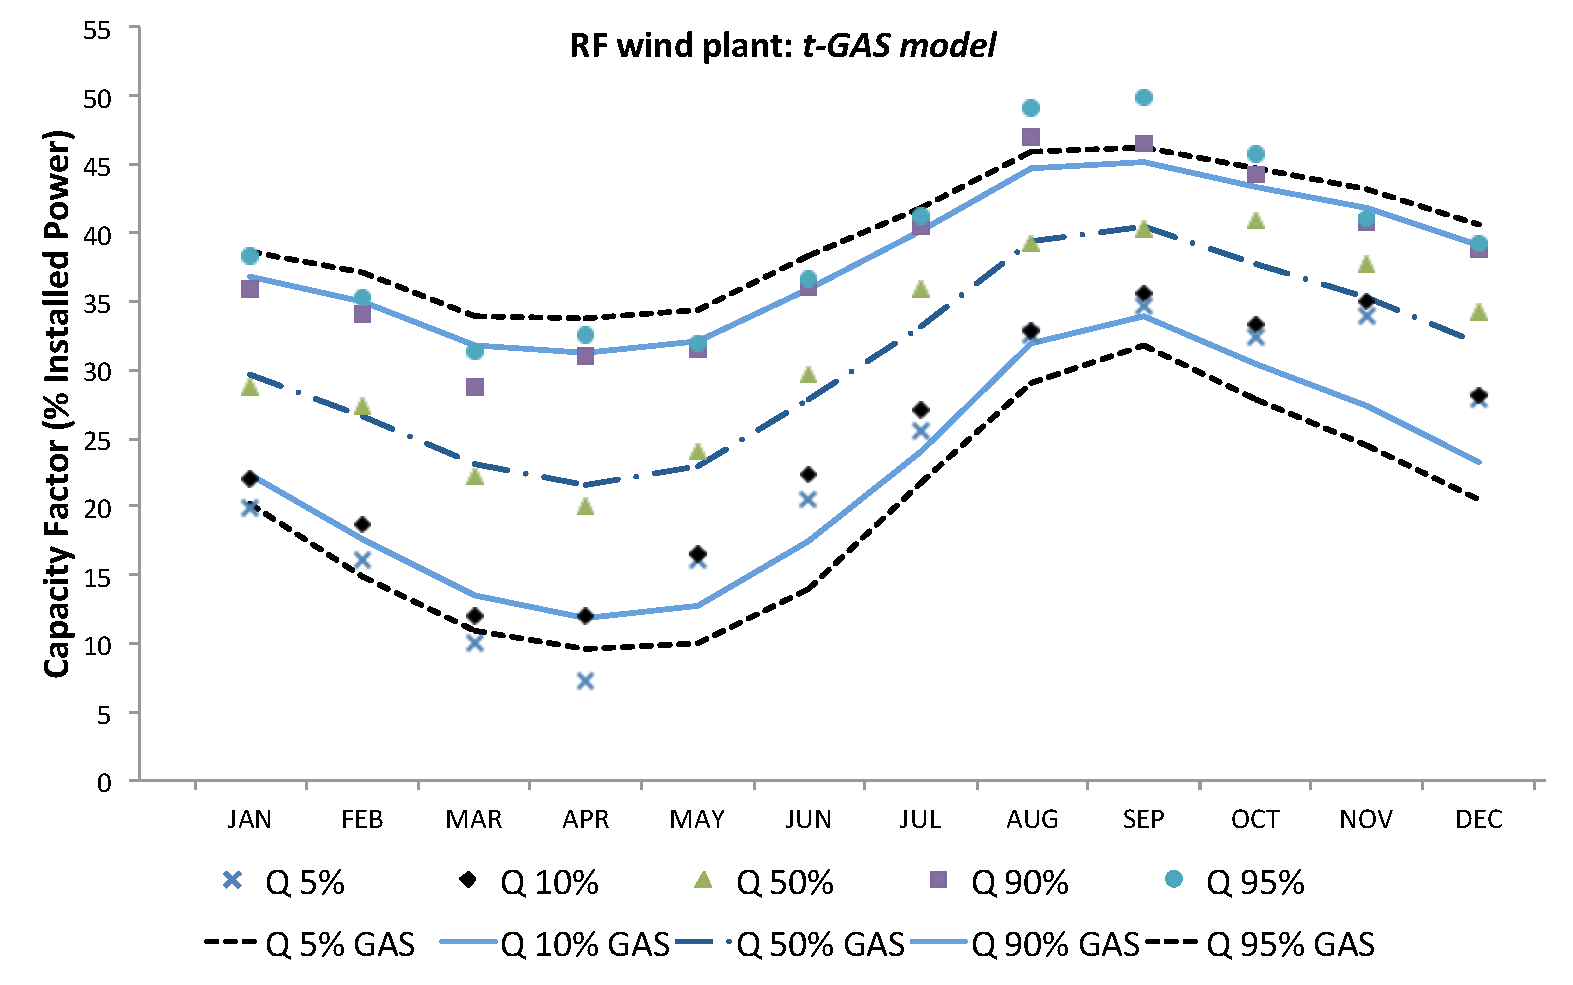
\includegraphics[height=5.5cm,width=9.0cm]{figures/RF_BETA_GAS.pdf}
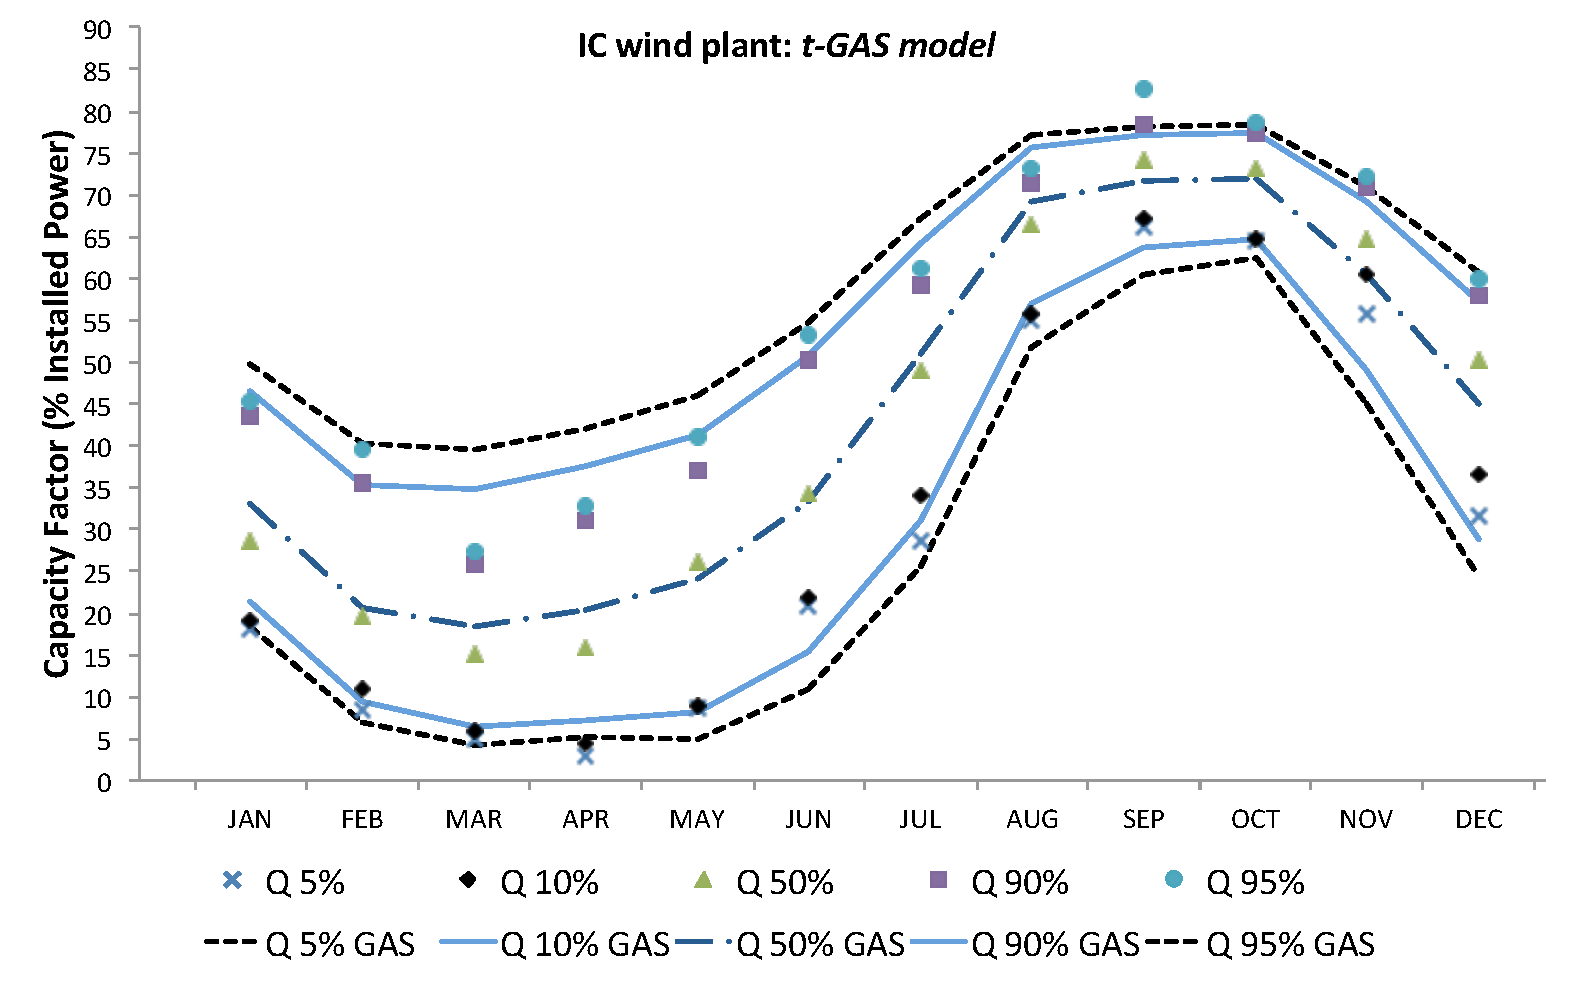
\includegraphics[height=5.5cm,width=9.0cm]{figures/IC_BETA_GAS.pdf}
%DIF > 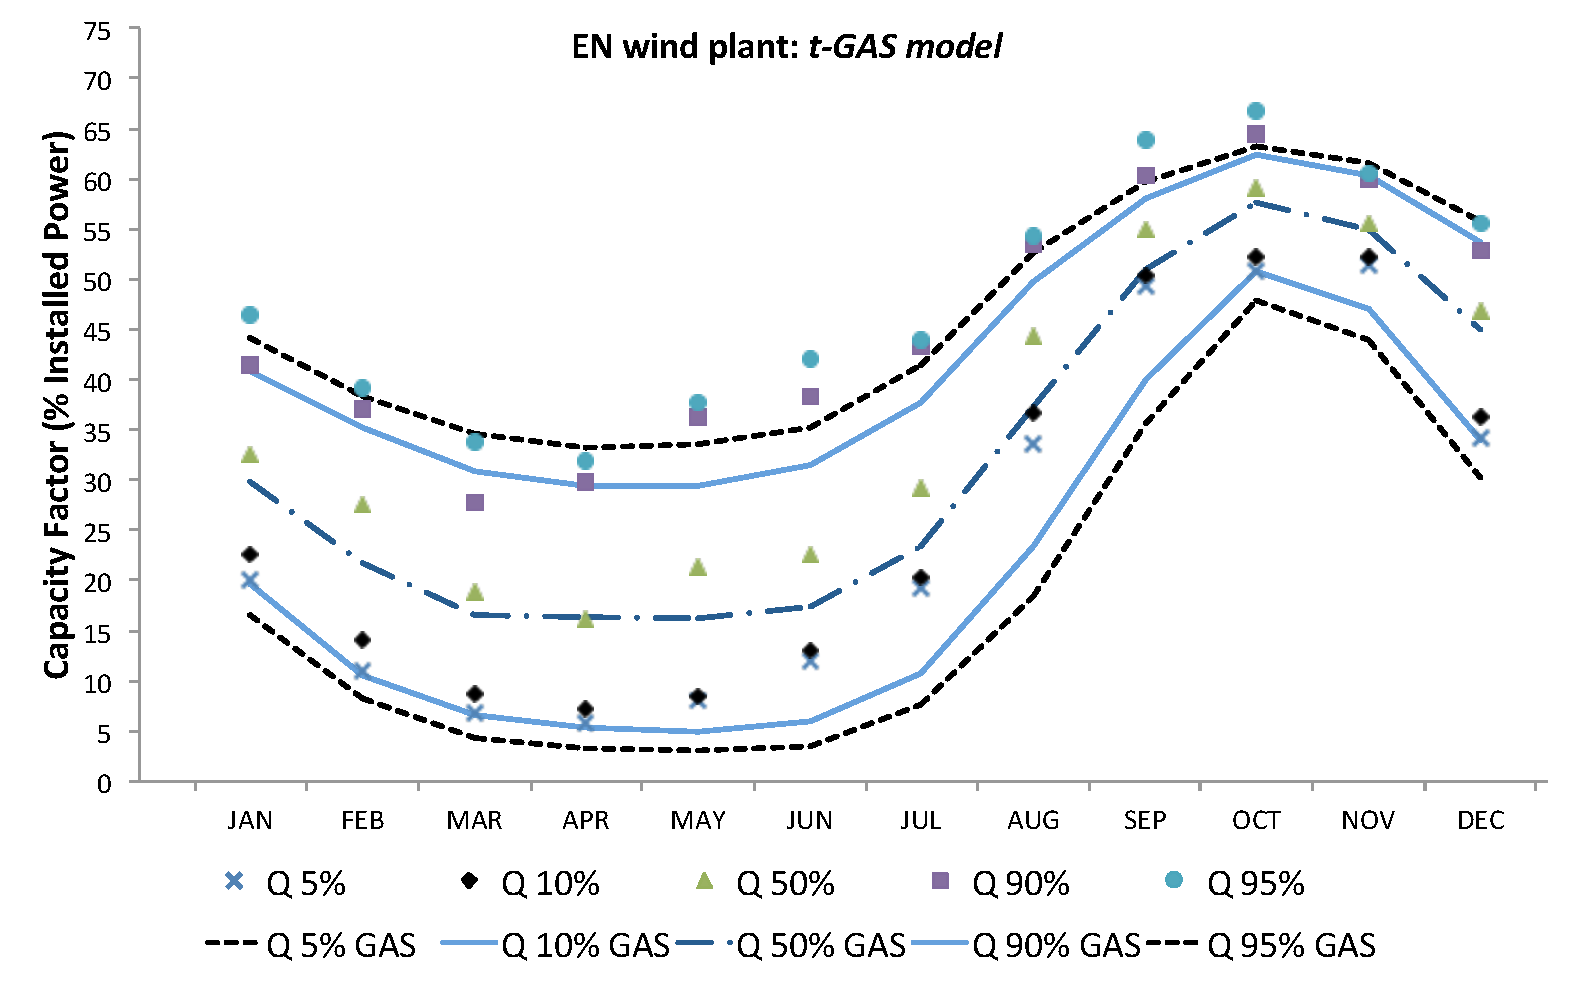
\includegraphics[height=5.5cm,width=9.0cm]{figures/EN_BETA_GAS.pdf}
\caption{\DIFaddFL{Scenario evaluation of the year of 2011 through beta }\emph{\DIFaddFL{t-GAS}} \DIFaddFL{model against the real data set.}}
\label{analise_cenarios_gas}
\end{figure}


\begin{figure}[htbp]
\centering
%DIF > 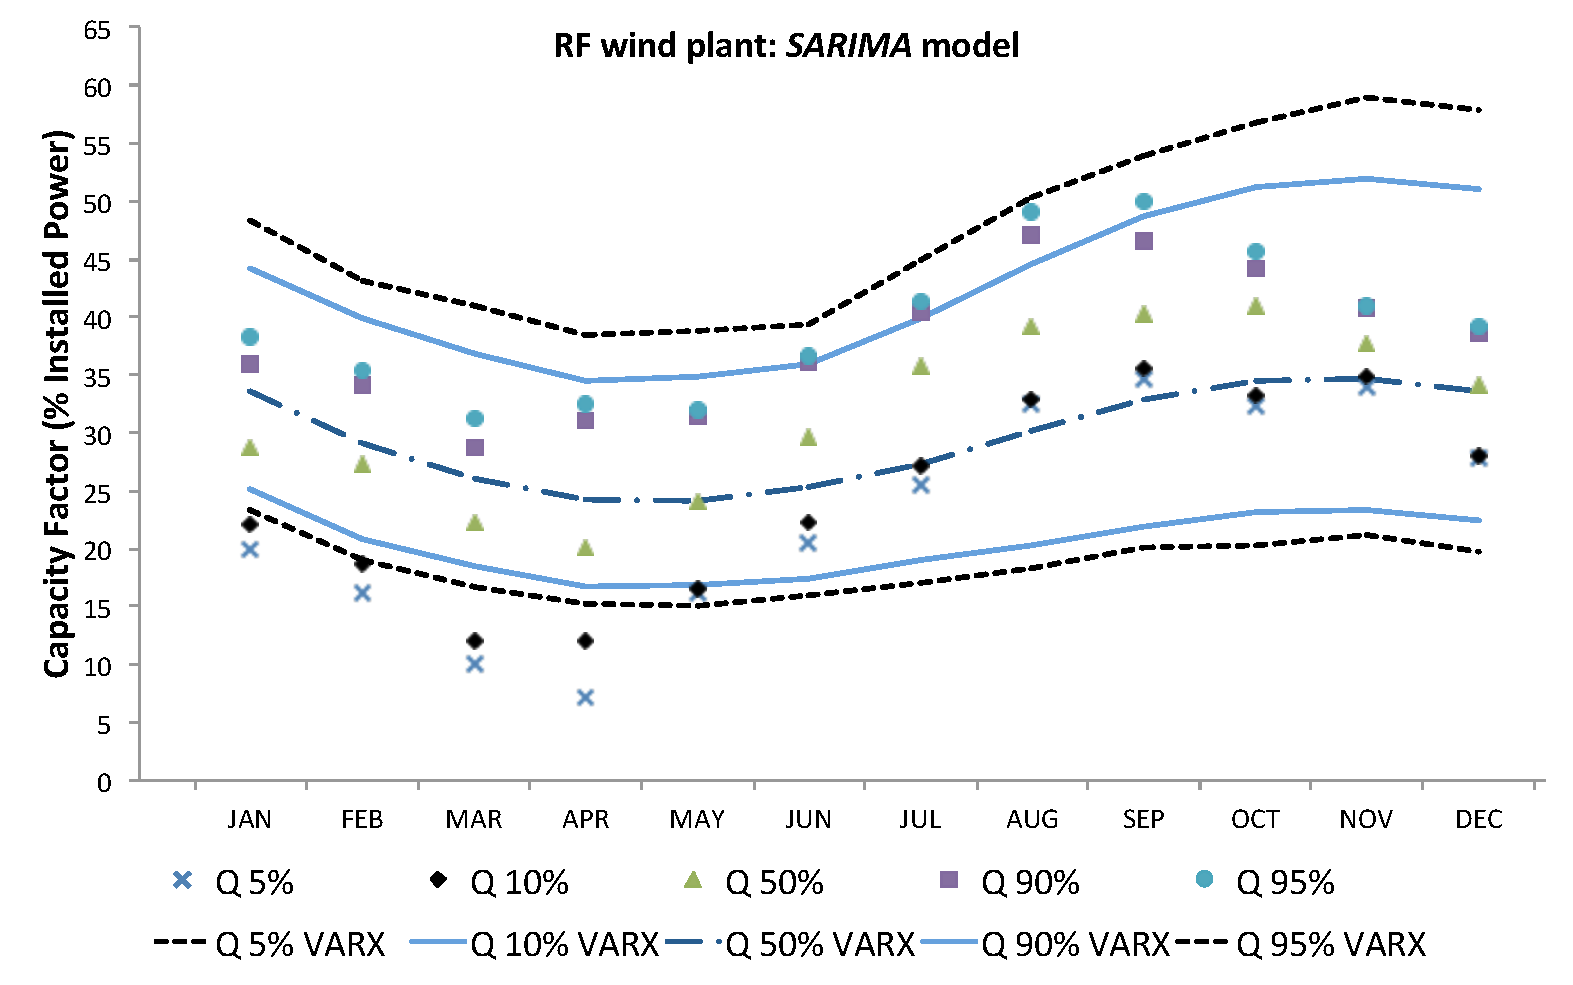
\includegraphics[height=5.5cm,width=9.0cm]{figures/RF_COM_LOG.pdf}
\includegraphics[height=5.5cm,width=9.0cm]{figures/IC_COM_LOG.pdf}
%DIF > 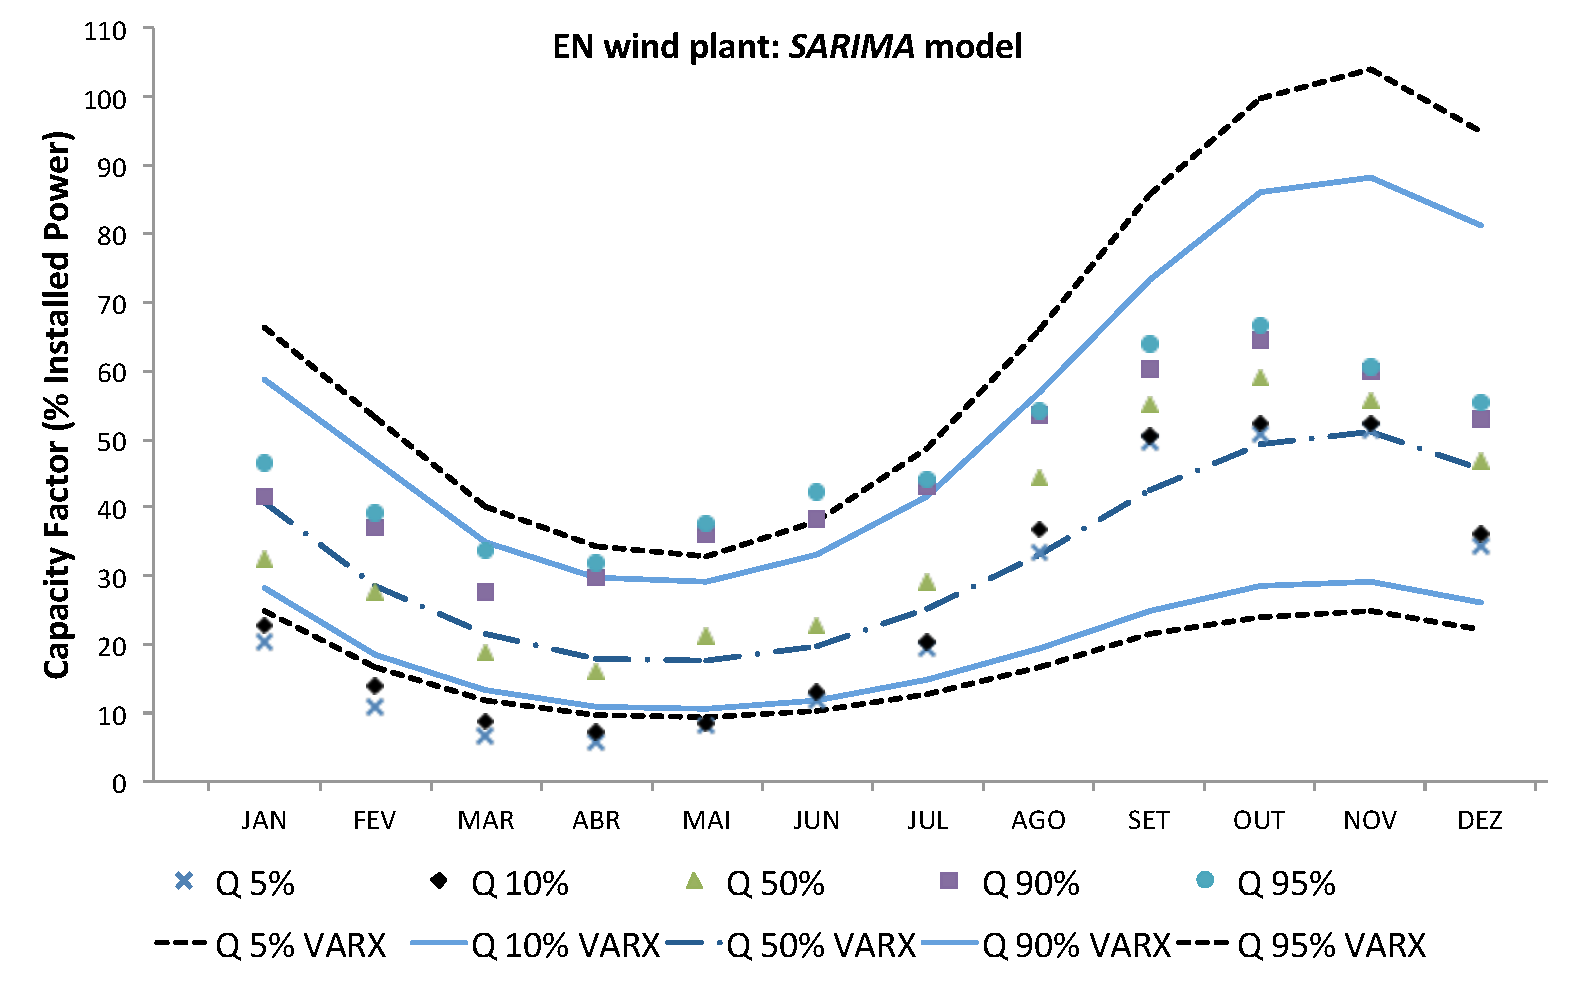
\includegraphics[height=5.5cm,width=9.0cm]{figures/EN_COM_LOG.pdf}
\caption{\DIFaddFL{Scenario evaluation of the year of 2011 through SARIMA model against the real data set.}}
\label{analise_cenarios_SARIMA}
\end{figure}

\DIFaddend Note that the quantiles from the simulated sets using our \DIFdelbegin \DIFdel{beta }\DIFdelend \emph{t-GAS} model \DIFdelbegin \DIFdel{are very close }\DIFdelend \DIFaddbegin \DIFadd{seems to be more reasonable and likely }\DIFaddend to the ones estimated from the real data set\DIFdelbegin \DIFdel{. These findings suggests that the simulated values produced by the beta }\emph{\DIFdel{t-GAS}} %DIFAUXCMD
\DIFdel{model seem to capture the correct underlying dependency structure presented in the wind CF time series . }\DIFdelend \DIFaddbegin \DIFadd{, while SARIMA ones are far beyond the historical quantiles. This provides evidences on the distortion brought by the anti log transformation, since we fitted a Gaussian SARIMA model to the log of the three WPG time series wind plants (EN,IC,RF).
}

\DIFaddend To reinforce our findings, we \DIFaddbegin \DIFadd{calculate the reliability of our quantiles as described in \mbox{%DIFAUXCMD
\cite{Wan2017}
}%DIFAUXCMD
. Low reliability on the extreme quantiles could prejudice the decision-making process. Based on the definition of quantile, the empirical proportion of quantile $q_t^\alpha$ is defined as,
}\begin{align}\DIFadd{ 
\hat{P}_Q^\alpha = \frac{1}{T}\sum_{t=1}^T \eta_t
}\end{align}
\noindent
\DIFadd{where T is the total number of observations, and $\eta_t$ denotes the indicator of quantiles $\hat{P}_Q^\alpha$ defined by,
}\begin{align}\DIFadd{ 
\eta_t=
\begin{cases}
1, }& \DIFadd{y_t \leq q_t^\alpha}\\
\DIFadd{0, }& \DIFadd{y_t > q_t^\alpha.}\\
\DIFadd{\end{cases}
}\end{align}

\DIFadd{The reability will provide the deviation between the empirical proportion $\hat{P}_Q^\alpha$ and nominal proportion $\alpha$ of the predicted quantiles. The average proportion deviation (APD) is then calculated by $\hat{PD}_Q^\alpha = \hat{P}_Q^\alpha - \alpha$ and provided in Table \ref{APD}. The closest to zero, the higher reability of the estimated quantiles $q_t^\alpha$.
}

\begin{table}[htbp]
\centering
\caption{\DIFaddFL{Average proportion deviation (APD)}}
\label{APD}
\begin{tabular}{@{}l|lll|lll@{}}
& \multicolumn{3}{c}{GAS}                                                  & \multicolumn{3}{c}{SARIMA}                                               \\  \hline
\DIFaddFL{$\alpha$ }& \multicolumn{1}{c}{RF} & \multicolumn{1}{c}{EN} & \multicolumn{1}{c}{IC} & \multicolumn{1}{c}{RF} & \multicolumn{1}{c}{EN} & \multicolumn{1}{c}{IC} \\ \hline
\DIFaddFL{5}\%   &     \DIFaddFL{3.33}\%            &  \DIFaddFL{3.33}\%               &   \DIFaddFL{3.33}\%                & \DIFaddFL{11.67}\%                &  \DIFaddFL{11.67}\%               &  \DIFaddFL{11.67}\% \\
\DIFaddFL{10}\%  &     \DIFaddFL{-1.67}\%            &  \DIFaddFL{6.67}\%               &   \DIFaddFL{6.67}\%               & \DIFaddFL{15.00}\%                &  \DIFaddFL{15.00}\%               &  \DIFaddFL{6.67}\%  \\
\DIFaddFL{50}\%  &     \DIFaddFL{3.33}\%            &  \DIFaddFL{8.33}\%               &  \DIFaddFL{8.33}\%                 & \DIFaddFL{16.67}\%                 &  \DIFaddFL{16.67}\%                &  \DIFaddFL{25.00}\%  \\
\DIFaddFL{90}\%  &     \DIFaddFL{1.67}\%            &   \DIFaddFL{1.67}\%               &  \DIFaddFL{-6.67}\%               & \DIFaddFL{10.00}\%                 &  \DIFaddFL{10.00}\%               &  \DIFaddFL{10.00}\% \\
\DIFaddFL{95}\%  &     \DIFaddFL{-3.33}\%           &  \DIFaddFL{-3.33}\%               &  \DIFaddFL{-3.33}\%               & \DIFaddFL{5.00}\%                 &  \DIFaddFL{5.00}\%                &  \DIFaddFL{5.00}\%  \\ \hline
\end{tabular}
\end{table}
%DIF > {\color{red} @PARADO AQUI: IR DIRETO PARA A DEFINICAO DE Q e falar do mecanismo de atualizacao}.
\DIFadd{By the results of Table \ref{APD} it is possible to argue that the scenarios generated by our proposed framework, specially on extreme quantiles, are very well estimated which is an expected outcome due to the fact that the copula model acts on the tail behaviour of the predictive density. In addition, we }\DIFaddend also implemented the conditional coverage Value at Risk exceedances test of \DIFdelbegin \DIFdel{Cristoffersen }\DIFdelend \DIFaddbegin \DIFadd{Christoffersen }\DIFaddend \cite{christoffersen1998evaluating} to check the coverage level of each predictive density against real data in Table \ref{cristofersen}. Non significant p-values reinforce the idea that the proposed model is \DIFdelbegin \DIFdel{not }\DIFdelend adequate to fit the \DIFdelbegin \DIFdel{CF }\DIFdelend \DIFaddbegin \DIFadd{WPG }\DIFaddend time series. 
\DIFdelbegin \DIFdel{As expected, p-values of Cristoffersen test applied to SARIMA predictive densities are all significant, considering a coverage level of 95}%DIFDELCMD < \%%%%
\DIFdel{. In contrast, predictive densities produced by beta }\emph{\DIFdel{t-GAS}} %DIFAUXCMD
\DIFdel{model are all non-significant, using the same level of coverage.
}%DIFDELCMD < 

%DIFDELCMD < %%%
\DIFdelend \begin{table}[htbp]
%\begin{table}[]
\centering
\caption{P-values conditional coverage Value at Risk exceedances test of Cristoffersen considering a coverage level of 95\%.}
\begin{tabular}{c|ccc}
\hline
{\bf Coverage level}      & {\bf \DIFdelbeginFL \DIFdelFL{Rio do Fogo}\DIFdelendFL \DIFaddbeginFL \DIFaddFL{RF}\DIFaddendFL } & {\bf \DIFdelbeginFL \DIFdelFL{Icaraizinho}\DIFdelendFL \DIFaddbeginFL \DIFaddFL{IC}\DIFaddendFL } & {\bf \DIFdelbeginFL \DIFdelFL{Enacel}\DIFdelendFL \DIFaddbeginFL \DIFaddFL{EN}\DIFaddendFL } \\ \hline
\emph{t-GAS} model   & \DIFdelbeginFL \DIFdelFL{0.306             }\DIFdelendFL \DIFaddbeginFL \DIFaddFL{0.305             }\DIFaddendFL & \DIFdelbeginFL \DIFdelFL{0.421           }\DIFdelendFL \DIFaddbeginFL \DIFaddFL{0.305           }\DIFaddendFL & 0.305        \\
SARIMA               & \DIFdelbeginFL \DIFdelFL{0.034             }\DIFdelendFL \DIFaddbeginFL \DIFaddFL{0.035             }\DIFaddendFL & 0.035           & \DIFdelbeginFL \DIFdelFL{0.011   }\DIFdelendFL \DIFaddbeginFL \DIFaddFL{0.035   }\DIFaddendFL \\ \hline     
\end{tabular}
\label{cristofersen}
\end{table}

%DIF < \begin{figure}[htbp]
\DIFdelbegin %DIFDELCMD < \begin{figure}[htbp]
%DIFDELCMD < \centering
%DIFDELCMD < 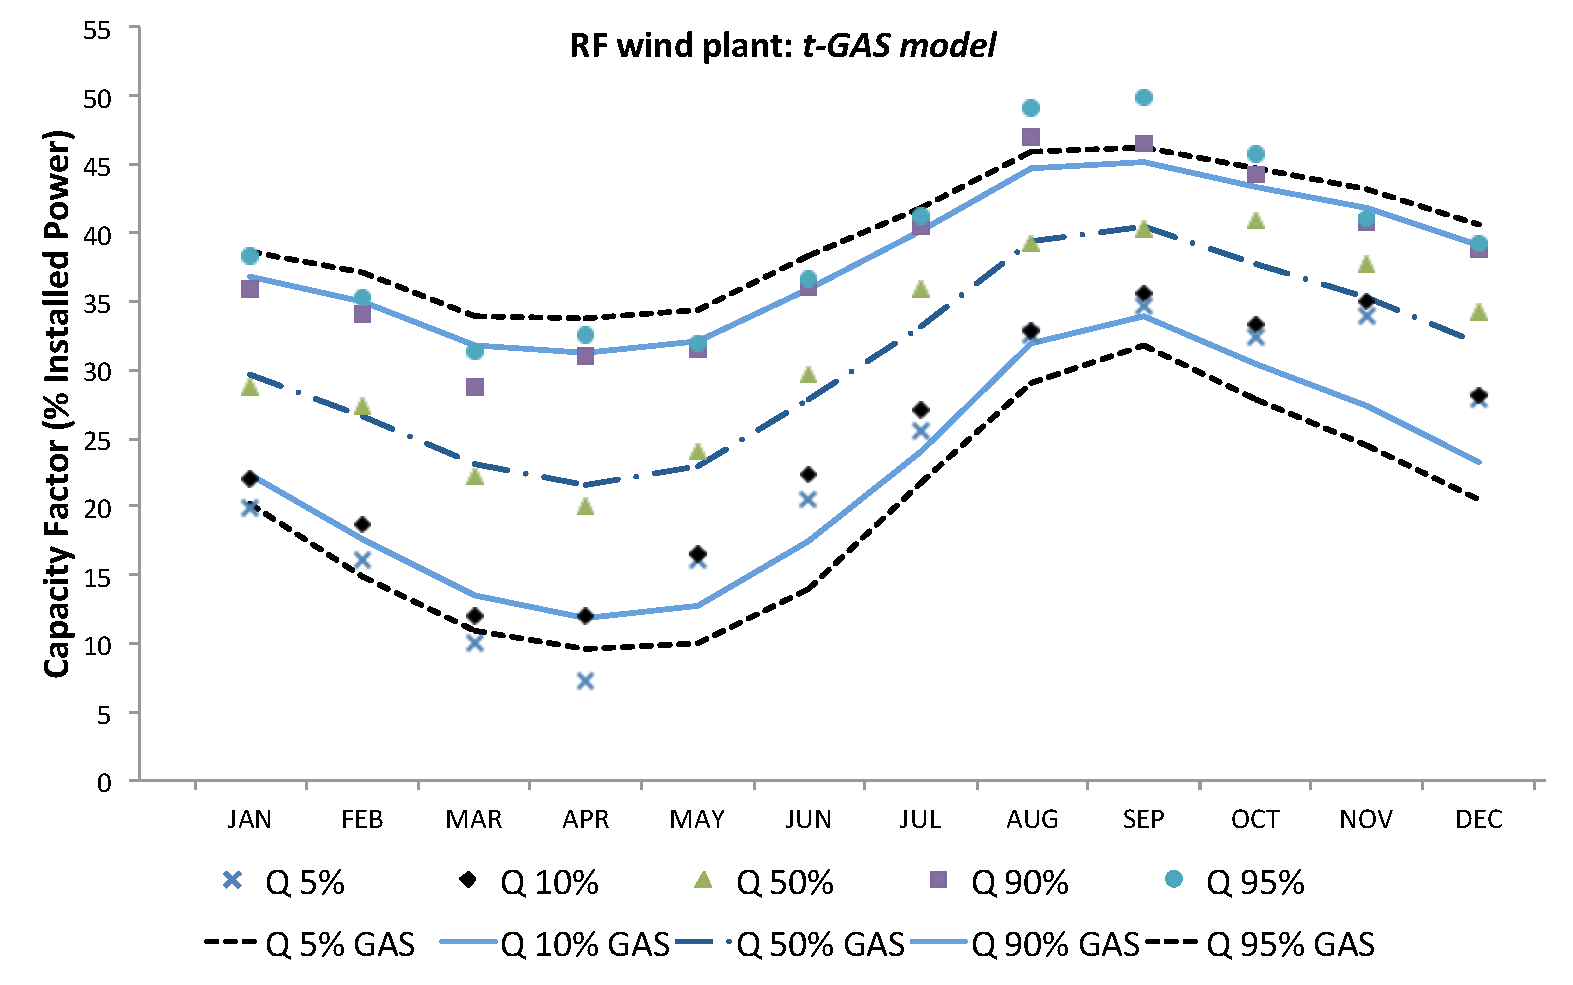
\includegraphics[height=5.5cm,width=9.0cm]{figures/RF_BETA_GAS.pdf}
%DIFDELCMD < 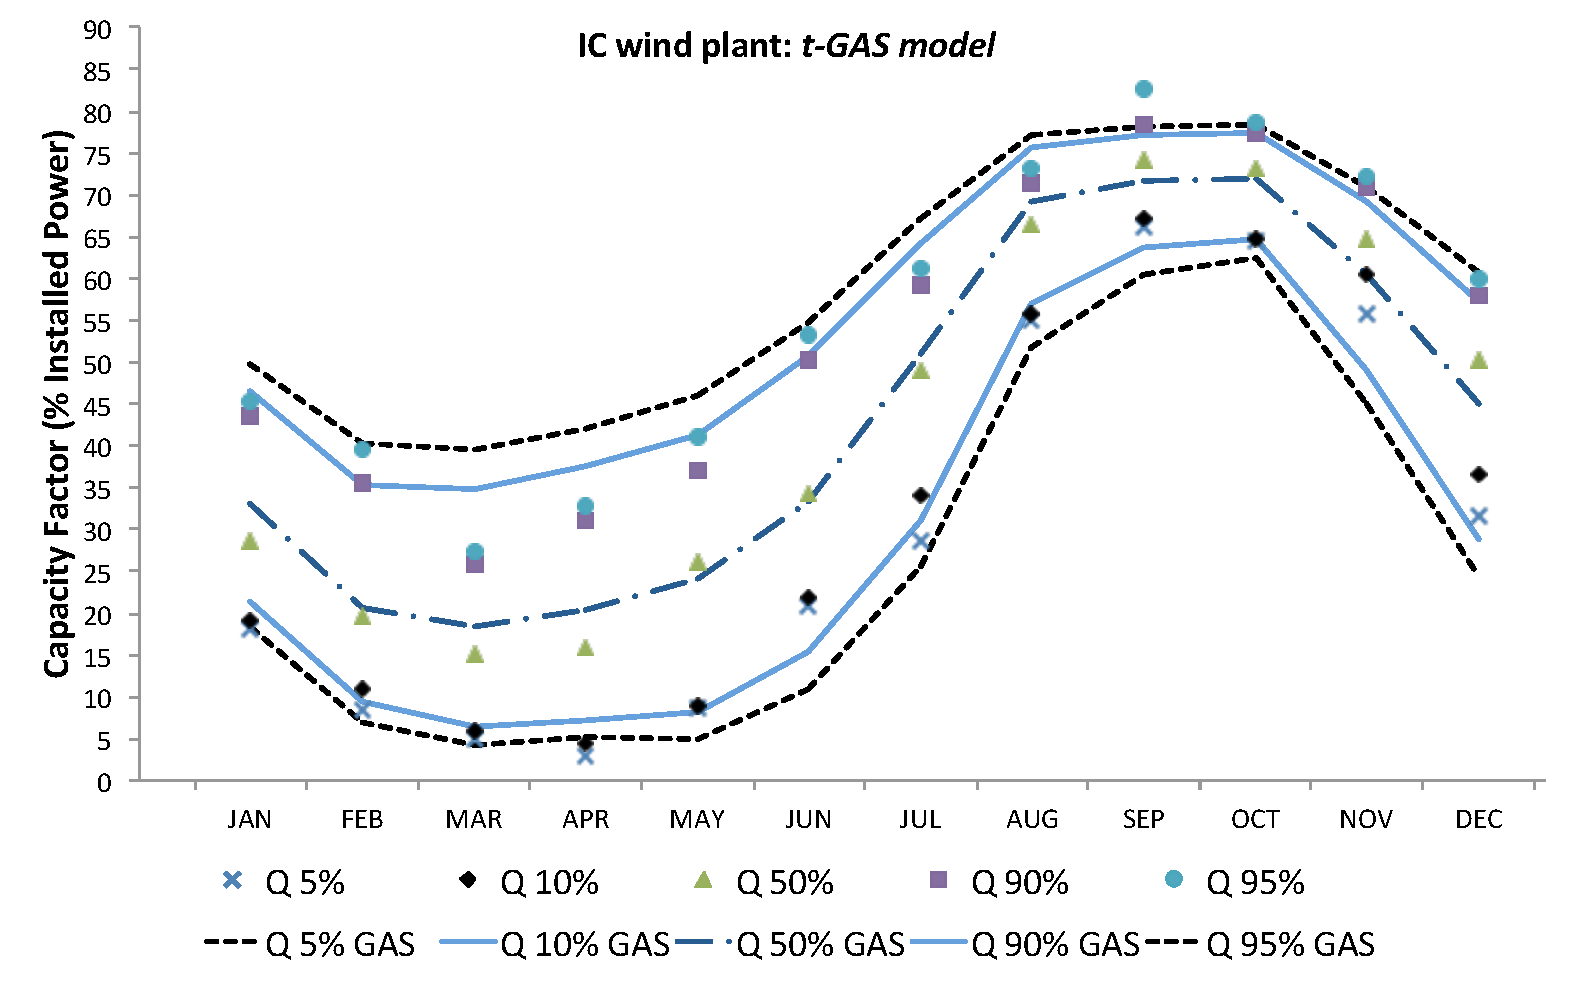
\includegraphics[height=5.5cm,width=9.0cm]{figures/IC_BETA_GAS.pdf}
%DIFDELCMD < 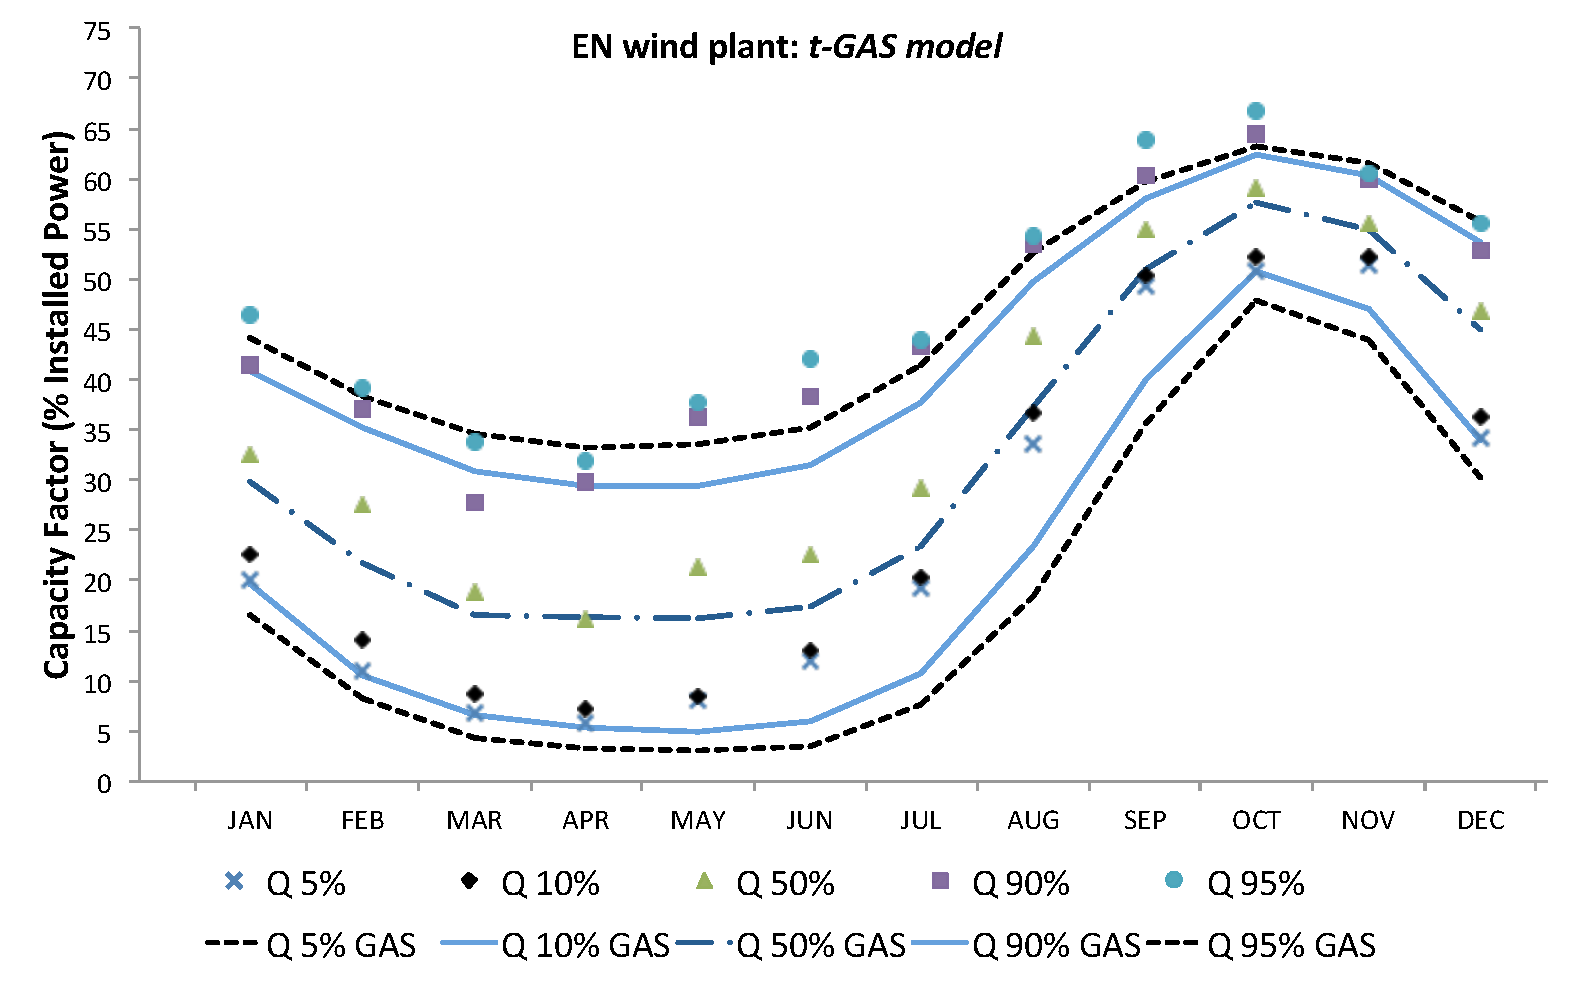
\includegraphics[height=5.5cm,width=9.0cm]{figures/EN_BETA_GAS.pdf}
%DIFDELCMD < %%%
%DIFDELCMD < \caption{%
{%DIFAUXCMD
\DIFdel{Scenario evaluation of the year of 2011 through beta }\emph{\DIFdel{t-GAS}} %DIFAUXCMD
\DIFdel{model against the real data set.}}
%DIFAUXCMD
%DIFDELCMD < \label{analise_cenarios_gas}
%DIFDELCMD < \end{figure}
%DIFDELCMD < 

%DIFDELCMD < \begin{figure}[htbp]
%DIFDELCMD < \centering
%DIFDELCMD < 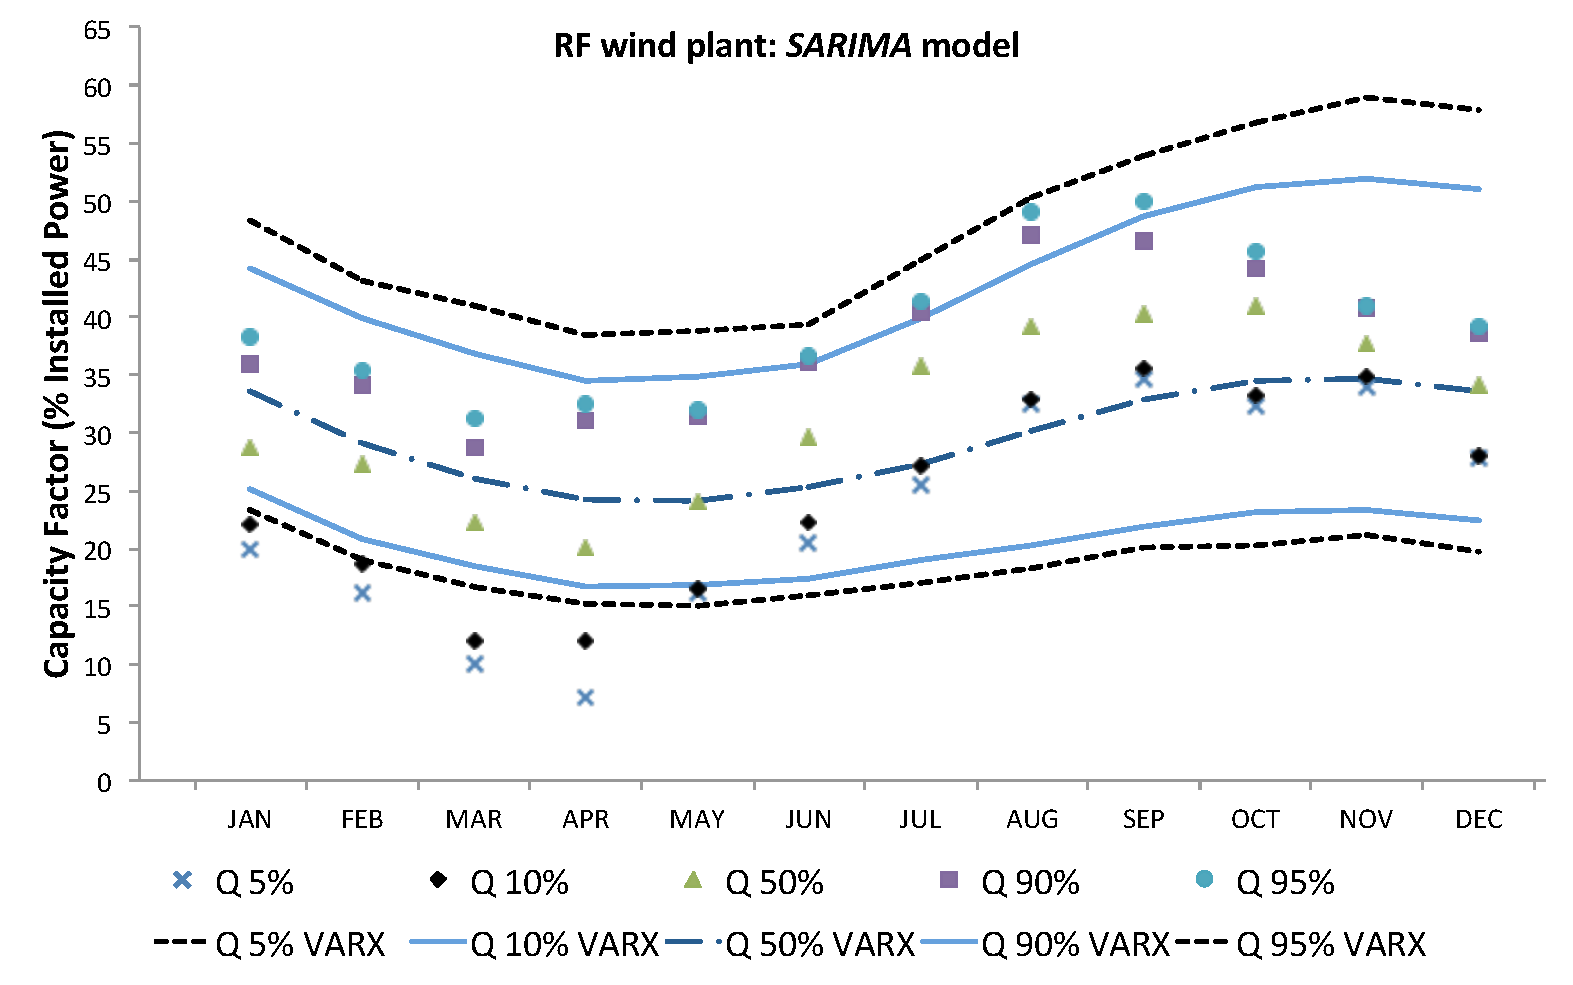
\includegraphics[height=5.5cm,width=9.0cm]{figures/RF_COM_LOG.pdf}
%DIFDELCMD < \includegraphics[height=5.5cm,width=9.0cm]{figures/IC_COM_LOG.pdf}
%DIFDELCMD < \includegraphics[height=5.5cm,width=9.0cm]{figures/EN_COM_LOG.pdf}
%DIFDELCMD < %%%
%DIFDELCMD < \caption{%
{%DIFAUXCMD
\DIFdel{Scenario evaluation of the year of 2011 through SARIMA model against the real data set.}}
%DIFAUXCMD
%DIFDELCMD < \label{analise_cenarios_SARIMA}
%DIFDELCMD < \end{figure}
%DIFDELCMD < 

%DIFDELCMD < %%%
\DIFdel{As already argued, such scenarios can benefit several areas. One of them is comercialization. For instance, in order to quantify the investor's risk at the Brazilian Free Trade Environment (FTE), first it is necessary to transform the capacity factors ($CF_{t}$) into energy generation in (}%DIFDELCMD < \%%%%
\DIFdel{) of firm energy certificate (${G}_{t}$). This is done by using the following formula
}\begin{align*}\DIFdel{
\tilde{G}_{i,t}=\frac{CF_{i,t}}{100}\cdot \frac{PoW_{i}}{FEC_{i}}, \label{eqrisk1}
}\end{align*}
%DIFAUXCMD
%DIFDELCMD < \noindent
%DIFDELCMD < %%%
\DIFdel{where $PoW_{i}$ and $FEC_{i}$ are respectively the power and the firm energy certificate of the wind plant $i\in I$.
Now, define $S=\lbrace 1,\ldots ,2000\rbrace $ are the scenarios generated independently from the Betas densities; $C={1,\ldots ,2000}$ are the scenarios obtained using the dependence structure as given by the Student t copula and $T=\lbrace 1,\ldots ,12\rbrace $ is the forecasting horizon for the risk evaluation for the year of 2011. At the most common contracts in the FTE, the so called quantity contracts, agents freely set a price of a bilateral contract where the seller compromises itself in delivering a fixed amount of energy $Q$, per period, in exchange of a fixed payoff (also per period). Still, in this setting, the contract represents only a financial instrument and does not impose a physical energy delivery obligation by the part of the seller. The differences between the energy due and the amount effectively generated are then settled at the spot market (by the spot price) at each period. In this sense, with $\tilde{G}_{t,i,z}$ and setting $z\in Z$, where $Z=\{S,C\}$ is the index that points out the aforementioned sets, it is possible to generate the distribution for a one year income obtained from a contract negotiated at the FTE. This is done by substituting $\tilde{G}_{t,i,z}$ as given in Equation }%DIFDELCMD < \eqref{eqrisk1}%%%
\DIFdel{, in the following equation: 
}\begin{align*}\DIFdel{
\tilde{R}_{t,i,z}=PQh_{t}+(\tilde{G}_{t,i,z}-Q) \tilde{\pi}_{t,z}h_{t}\,\, \mbox{for}\,\, t \in T, \label{eqrisk2}
}\end{align*}
%DIFAUXCMD
%DIFDELCMD < \noindent
%DIFDELCMD < %%%
\DIFdel{where $\tilde{\pi}_{t,z}$ denotes the spot price at configuration $z$ at each period of the contract's horizon, $h_{t}$ is the total number of hours of period $t$; $Q$ is the amount of energy sold through the bilateral contract, in avg-MW and , $P$ is the price that defines the contract's fixed payoff parcel at each period. The latter two quantities are fixed at $P=100$ R}%DIFDELCMD < \$%%%
\DIFdel{/MWh and $Q=1AvgMW$. The net present value (NPV) of each contract is then given by }\begin{align*}\DIFdel{
\tilde{R}_{i,z}=\sum_{t\in T}{\frac{\tilde{R}_{t,i,z}}{(1+K)^{t}}}\,\, \mbox{for} \,\, i\in I
}\end{align*}
%DIFAUXCMD
\DIFdel{where $K$ is the interest rate, wich is fixed in zero. Now to generate the distribution of the NPV of the portfolio with contracts attached to those three wind plants, it is only necessary to substitute in Equation }%DIFDELCMD < \eqref{eqrisk2} %%%
\DIFdel{the variable $\tilde{G}_{t,i,z}$ for $\sum_{t\in T}{\sum_{i\in I}{\tilde{G}}_{t,i,z}}$. After that, to obtain the distribution of the cash-flow generated by this portfolio, one just adds their values, as given by 
  Equation }%DIFDELCMD < \eqref{eqrisk2}%%%
\DIFdel{, resulting in
}\begin{align*}\DIFdel{
\tilde{R}_{z}^{Port}=\sum_{t\in T}{\sum_{i\in I}{\tilde{R}_{t,i,z}}}.
}\end{align*}
%DIFAUXCMD
%DIFDELCMD < 

%DIFDELCMD < %%%
\DIFdel{The CVaR estimated using the simulated distribution of the cash flows associated with this portfolio are presented in Table \ref{CVar_rendas}, where ``dependent'' refers to those scenarios generated through the Student t copula, and ``independent'',refers to simulations obtained directly from each of the beta marginal models.
 }%DIFDELCMD < \begin{table}%%%
%DIF < [H]
 %DIFDELCMD < \centering
%DIFDELCMD < %%%
%DIF <  \small
 %DIFDELCMD < \caption{%
{%DIFAUXCMD
\DIFdel{CVaR for the distribution of cash flows for different portfolios.}}
 %DIFAUXCMD
%DIFDELCMD < \begin{tabular}{|c|c|c|c|c|}
%DIFDELCMD <  \hline
%DIFDELCMD <  {%%%
\DIFdel{$CVaR^{95\%}$}%DIFDELCMD < } & %%%
\DIFdel{Dependent }%DIFDELCMD < & %%%
\DIFdel{Independent }%DIFDELCMD < \\ \hline
%DIFDELCMD < %%%
%DIF <  \midrule
 \DIFdel{$\tilde{R}_{RF,z}$ }%DIFDELCMD < & %%%
\DIFdel{-967.06 }%DIFDELCMD < & %%%
\DIFdel{-1,051.00 }%DIFDELCMD < \\ \hline
%DIFDELCMD <  %%%
\DIFdel{$\tilde{R}_{IC,z}$ }%DIFDELCMD < & %%%
\DIFdel{490.31 }%DIFDELCMD < & %%%
\DIFdel{316.79 }%DIFDELCMD < \\ \hline
%DIFDELCMD <  %%%
\DIFdel{$\tilde{R}_{EN,z}$ }%DIFDELCMD < & %%%
\DIFdel{622.79 }%DIFDELCMD < & %%%
\DIFdel{467.27 }%DIFDELCMD < \\ \hline
%DIFDELCMD <  %%%
\DIFdel{$\tilde{R}_{z}^{Port}$ }%DIFDELCMD < & %%%
\DIFdel{1,224.39 }%DIFDELCMD < & %%%
\DIFdel{1, 093.95 }%DIFDELCMD < \\ \hline
%DIFDELCMD < %%%
%DIF <  \bottomrule
 %DIFDELCMD < \end{tabular}%%%
%DIF < 
 %DIFDELCMD < \label{CVar_rendas}%%%
%DIF < 
 %DIFDELCMD < \end{table}%%%
%DIF < 
%DIFDELCMD < 

%DIFDELCMD < %%%
\DIFdel{We focus our attention on the CVaR of $\tilde{R}_{z}^{Port}$. Such a figure indicates that by considering dependence between the CF's of the different wind plants, one obtains an increase of 12}%DIFDELCMD < \% %%%
\DIFdel{on this risk measure compared to the risk evaluated by not taking into account dependence. In the present context this means that an investor would experience a 12}%DIFDELCMD < \% %%%
\DIFdel{increase on his/her income when investing in such portfolio. Also the CVaR from the wind plant IC, $\tilde{R}_{2,v}$, presents the largest difference when comparing dependent with independent scenarios, 54.7}\DIFdelend \DIFaddbegin \DIFadd{As expected, p-values of Cristoffersen test applied to SARIMA predictive densities are all significant, considering a coverage level of 95}\DIFaddend \%. %DIF < These results indicate that the proposed approach figures as an alternative to that of the VARX model to generate integrated scenarios of wind capacity factor, where the simulation can be done only by one step.
\DIFaddbegin \DIFadd{In contrast, predictive densities produced by }\emph{\DIFadd{t-GAS}} \DIFadd{model are all non-significant, using the same level of coverage.
}\DIFaddend 

% ===== Sec. V - Conclusion ===== %

\section{Conclusion}\label{Conclusion}

\DIFdelbegin \DIFdel{Our methodology for simulate scenarios from a joint density of wind capacity factor seems fruitful and have several benefits when comparing to the models presented in the  literature so far. First,
we propose a non Gaussian model to filter wind CF dynamic. By doing such, one does not need to transform variables and work with the $log$ of the observed data point, our framework is taylor made for the range of values that CF's time series can assume. In addition, the simulated values will be always inside physical limits of production, i. e. , it will never assume values bigger than the maximum production of wind plant $i$.
}%DIFDELCMD < 

%DIFDELCMD < %%%
\DIFdel{The results presented in this work indicates that our methodology figures as an alternative to simulate joint scenarios of renewable energy sources, where the simulation can be done only by one step.
}%DIFDELCMD < 

%DIFDELCMD < %%%
%DIF < \section*{Acknowledgment}
\DIFdelend \DIFaddbegin \DIFadd{In this paper we proposed a framework to simulate joint scenarios of WPG time series taking into account the spatial dependence among different units. Such scenarios are deeply demanded for the development of medium- and long-term studies for power-system planning under uncertainty of renewable energy generation. Our methodology seems fruitful and have several benefits when comparing against a benchmark SARIMA model, regarding its parametric features and the straightforward way to estimate and generate extreme quantiles. The proposed framework was derived making use of a recently proposed class of time-series models with time-varying parameters and arbitrary non Gaussian distribution, known as Generalized Auto Regressive Score models (GAS). When adopting such models, one does not need to transform WPG and work with the $log$ of the observed data point. Our framework is taylor made for the range of values that WPG time series can assume. In addition, copula models were used to input spatial dependence into the generated joint scenarios. Its use is unarguably better when comparing the extreme scenarios to the ones generated by the SARIMA model.
}\section*{\DIFadd{Acknowledgment}}
\DIFaddend 

%DIF < The authors would like to thank FICO (Xpress-MP developer) for the academic partnership program with the Electrical Engineering Department of Pontifical Catholic University of Rio de Janeiro, Brazil (PUC-Rio). The authors would also like thank the LAMPS researchers for the daily exchanges and their insightful considerations.
\DIFaddbegin \DIFadd{Henrique Hoeltgebaum, Cristiano Fernandes and Alexandre Street acknowledge support from CNPq/Brazil.
}\DIFaddend 

%\IEEEtriggeratref{17}
\bibliographystyle{IEEEtran}
\bibliography{Bibhenriquinho}

%DIF < \begin{IEEEbiographynophoto}{Bruno Fanzeres} (S'11) has a B.Sc. degree in Electrical and Industrial Engineering and a M.Sc. degree in Operations Research from PUC-Rio, Brazil. He is pursuing a Ph.D degree in Operations Research at the same university.
%DIF > \begin{IEEEbiographynophoto}{Henrique Hoeltgebaum} has a B.Sc. degree in Statistics from Federal University of Rio Grande do Sul, Brazil and a M.Sc. degree in Electrical Engineering from PUC-Rio, Brazil. Currently he is pursuing a Ph.D degree in Electrical Engineering at the same university.
%\end{IEEEbiographynophoto}

%DIF < \begin{IEEEbiographynophoto}{Arthur Brigatto} (S'14) received a B.Sc. degree in Electrical Engineering from the Federal University of Juiz de Fora, Brazil, and is pursuing a M.Sc. in Electrical Engineering at PUC-Rio, Brazil.
%DIF > \begin{IEEEbiographynophoto}{Cristiano Fernandes} has a M.Sc. degree in Electrical Engineering from PUC-Rio, Brazil and a D.Sc. in Statistics from London School of Economics.
%\end{IEEEbiographynophoto}

%\begin{IEEEbiographynophoto}{Alexandre Street} (S'06, M'10) holds the degrees of M.Sc. and D.Sc. in Electrical Engineering (Operations Research) from PUC-Rio, Brazil. 
%\end{IEEEbiographynophoto}

%DIF < \begin{IEEEbiographynophoto}{Luiz Augusto Barroso} (S'00, M'06, SM'07) has a B.Sc. in Mathematics and a Ph.D degree in Operations Research. He is a technical director at PSR.
%DIF < \end{IEEEbiographynophoto}
\DIFaddbegin \appendices

\section{\DIFadd{Gas mechanism for the multivariate Student t distribution}}\label{FirstAppendix}

\DIFadd{In this appendix we present the elements of the GAS mechanism $s_t$, $\nabla_{t}$ and $\mathcal{I}_{t|t-1}^{-1}$ for the multivariate Student t distribution, but first let us define a few matrix notations. The matrix $\mathcal{D}_{K}$ is a duplication matrix given by $\mathcal{D}_{K}vech(C) = vec(C)$ and the Kronecker product of two matrixes $C$ and $D$ is denoted by $C \otimes D$. In case $C=D$, $C_{\otimes}$. By convenience the operator $vec(C)$ creates a column vector from a matrix $C$ by stacking the column vectors of $C$ while $vech(C)$ also creates a column vector stacking only column vectors of the inferior triangular part of $C$. For a full detailed review on linear algebra operators, please see \mbox{%DIFAUXCMD
\cite{abadir2005matrix}
}%DIFAUXCMD
.
}

\DIFadd{Now, the proposed GAS mechanism in\mbox{%DIFAUXCMD
\cite{creal2011dynamic}
}%DIFAUXCMD
to update the time varying correlation matrix $\Sigma_t$ using a multivariate Student t is given by 
  }

\begin{align}\DIFadd{ 
\nabla_{t} = \frac{\partial \ln p(\tilde{y}_{t}|\Sigma_{t};\nu)}{\partial f_{t}} =}& \DIFadd{\frac{1}{2} \Psi_{t}^{'} \mathcal{D}_{K}^{'}\Sigma_{t\otimes}^{-1}[w_{t}\tilde{y}_{t\otimes}-vec(\Sigma_{t})] \label{nabla} }\\
\DIFadd{\mathcal{I}_{t|t-1} = E}[\DIFadd{\nabla_{t}\nabla_{t}^{'}}] \DIFadd{=}& \DIFadd{\frac{1}{4} \Psi_{t}^{'} \mathcal{D}_{K}^{'}J_{t\otimes}^{'}[gZ-vec(I)vec(I)^{'}] \label{info} }\\ & \DIFadd{J_{t\otimes}\mathcal{D}_{K}\Psi_{t} \nonumber
}\end{align}
\noindent
\DIFadd{where $\Psi_{t}=\partial vech(\Sigma_{t})/\partial f_{t}^{'}$ which will be presented next in Equation }\eqref{derivPSI}\DIFadd{, the scalar $w_{t}=(\nu+K)/(\nu-2+\tilde{y}_{t}^{'}\Sigma_{t}^{-1}\tilde{y}_{t})$ reduces the effects of outliers, once the former quantity is divided by $\tilde{y}_{t}^{'}\Sigma_{t}^{-1}\tilde{y}_{t}$. Matrix $J_{t}$ is defined as $\Sigma^{-1}_{t}=J^{'}_{t}J_{t}$, which can be obtained by any matrix decomposition procedure. In our application in Section \ref{Application}, we adopted Cholesky decomposition. The scalar $g=(\nu+K)/(\nu+2+K)$ and the elements of the square matrix $Z$ of dimension $K\times K$, are given by
}\begin{align}\DIFadd{ 
Z}[\DIFadd{(i-1)\cdot k+\ell,(j-1)\cdot k+m}]\DIFadd{=\delta_{ij}\delta_{\ell m} + \delta_{i\ell}\delta_{j m} +  \delta_{im}\delta_{j \ell}
}\end{align}
\noindent
\DIFadd{with $i,j,\ell,m=1,...,K$, assuming $\delta_{ij}$ equals to 1 if $i=j$ and zero otherwise. 
}

\DIFadd{As previously discussed, the key to define a copula framework in \mbox{%DIFAUXCMD
\cite{creal2011dynamic}
}%DIFAUXCMD
is to use the following specification of $\Psi_{t}$ in Equations }\eqref{nabla}\DIFadd{-}\eqref{info}\DIFadd{,
}\begin{equation}\DIFadd{ \label{derivPSI}
\Psi_{t} = \mathcal{B}_{K}D_{t\otimes}\Delta^{-1}_{t\otimes}[\mathcal{D}_{K}-(\Delta_{t} \oplus Q_{t})\Delta_{t\otimes}^{-1}W_{\Delta_{t}}\mathcal{S}_{\Delta}]\mathcal{S}_{Q}
}\end{equation}
\noindent
\DIFadd{where $\mathcal{S}_{Q}=I$ since $f_{t}=vech(Q_{t})$. The matrix $W_{\Delta_{t}}$ is initially calculated using a diagonal matrix of dimension $K^{2} \times K^{2}$ with elements of the main diagonal equals to $0.5vec(\Delta^{-1}_{t})$, and later the columns of zeros are eliminated. The matrix $\mathcal{S}_{\Delta}$ is a selection matrix, with ones and zeros, given by $diag(\Delta^{2}_{t})=\mathcal{S}_{\Delta}vech(Q_{t})$. The operator $\oplus$ is given by $C\oplus D=(C\otimes D)+(D\otimes C)$. In addition, $\mathcal{B}_{K}=(\mathcal{D}_{K}^{'}\mathcal{D}_{K})^{-1}\mathcal{D}_{K}^{'}$ is a duplication matrix composed by only zeros and ones, with more lines than columns. $\Delta_{t}$ is a diagonal matrix which elements are the square root of the elements contained in the main diagonal of $Q_{t}$
}\DIFaddend 

\end{document}
